
\chapter{From Reservoir Embeddings to Graph-Based Clinical EEG Analysis}
\label{chap:arspi_net}

\section{Introduction}
\label{sec:ch5_intro}

The preceding chapters established the reservoir component of ARSPI-Net as a nonlinear temporal feature extractor for single-channel EEG. Chapter~\ref{ch:lsm_experiments} validated the Leaky Integrate-and-Fire reservoir under controlled conditions, and Chapter~\ref{ch:lsm_embeddings} demonstrated that binned spike-count features (BSC$_6$), reduced to sixty-four principal components, provide a compact and discriminative embedding for each electrode channel. The present chapter asks the next question in the pipeline: how should these channel-wise embeddings be coupled across the multichannel EEG array so that inter-electrode structure can be exploited for both classification and scientific interpretation?

This chapter pursues three interleaved scientific questions on the full $211$-subject SHAPE dataset. The first is a representation question: how much of the reservoir embedding space is occupied by condition-related signal versus subject-identity nuisance structure? The second is a graph-propagation question: under what finite-sensor graph conditions does message-passing propagation increase or decrease the detectability of a weak condition signal embedded in strong subject-level noise? The third is a clinical-topological question: when the same graph is analyzed descriptively rather than propagatively, what transdiagnostic network phenotypes emerge?

The experimental program produces three principal findings. First, variance decomposition reveals that subject identity accounts for $62.6\%$ of embedding variance, condition accounts for $8.7\%$, and residual within-subject variability accounts for $28.7\%$---a $7\times$ subject-to-condition dominance ratio. Removing the subject-identity component through per-subject centering increases classification accuracy from $63.4\%$ to $79.4\%$ balanced accuracy, a $+16.0$ percentage-point gain that reveals the condition signal is substantially richer than the original representation suggests. Second, a Propagation Operating Characteristic analysis across six graph densities and six propagation depths demonstrates that message-passing monotonically reduces classification accuracy at every density tested, absorbing up to $90\%$ of inter-channel discriminative variance at high density. This regime boundary is robust across Pearson, spatial-distance, and random graph constructions. Third, graph-topological analysis, applied descriptively to the same graphs, reveals that Substance Use Disorder modulates emotional network reactivity across three complementary metrics, validated through permutation testing and internal replication at two sample sizes.

The chapter is organized as follows. Sections~\ref{sec:ch5_gnn_theory}--\ref{sec:ch5_dataset} present the theoretical framework and dataset. Section~\ref{sec:ch5_raw_obs} characterizes the raw data at every pipeline stage. Section~\ref{sec:ch5_classification} presents the classification experiments. Section~\ref{sec:ch5_variance} develops the variance decomposition, subject-nuisance suppression, and detection-theoretic analyses. Section~\ref{sec:ch5_regime} presents the Propagation Operating Characteristic and graph construction sweep. Sections~\ref{sec:ch5_interpretability}--\ref{sec:ch5_nonrep} demonstrate that graph-topological analysis provides a transdiagnostic clinical interpretability tool. Sections~\ref{sec:ch5_novelty}--\ref{sec:ch5_summary} discuss novelty, significance, and the bridge to Chapter~\ref{ch:dynamics}.


\section{Theoretical Foundations}
\label{sec:ch5_gnn_theory}

\subsection{Graph Representation of Multichannel EEG}

A multichannel EEG recording can be represented as a graph $\mathcal{G} = (\mathcal{V}, \mathcal{E}, \mathbf{X})$ where the node set $\mathcal{V} = \{v_1, \ldots, v_C\}$ corresponds to $C = 34$ electrode channels, the edge set $\mathcal{E}$ encodes pairwise relationships, and the node feature matrix $\mathbf{X} \in \mathbb{R}^{C \times d}$ collects the per-channel PCA-64 embeddings. The adjacency matrix is constructed by thresholding the Pearson correlation between channel embeddings:
\begin{equation}
    A_{ij} = \mathbf{1}\left[\rho(\mathbf{x}_i, \mathbf{x}_j) \geq \tau_\rho\right],
\end{equation}
where $\tau_\rho$ retains the top $20\%$ of channel pairs, yielding approximately $112$ edges at $20\%$ density.

\subsection{Message-Passing Neural Networks}

The message-passing framework \cite{Gilmer2017} updates node representations through iterative neighborhood aggregation:
\begin{equation}
    \mathbf{h}_v^{(k+1)} = \psi^{(k)}\!\left(\mathbf{h}_v^{(k)},\; \bigoplus_{u \in \mathcal{N}(v)} \phi^{(k)}\!\left(\mathbf{h}_u^{(k)}, \mathbf{h}_v^{(k)}, \mathbf{e}_{uv}\right)\right).
\end{equation}
Three architectures are evaluated: GCN \cite{Kipf2017} (normalized adjacency aggregation), GIN \cite{Xu2019} (sum-aggregation with MLP, maximally expressive under the Weisfeiler-Lehman test), and EdgeConv \cite{Wang2019} (edge-feature MLP with max-aggregation). For graph-level classification, mean-max pooling produces the graph representation $\mathbf{z} = [\text{mean}(\mathbf{H}^{(K)}) \| \max(\mathbf{H}^{(K)})]$.

\subsection{Graph-Topological Descriptors}

Beyond classification, the graph admits topological descriptors: global efficiency $E_{\text{glob}} = \frac{1}{C(C-1)} \sum_{i \neq j} d_{ij}^{-1}$ (network integration), mean clustering coefficient $\bar{C}$ (local redundancy), degree heterogeneity (coefficient of variation of degrees), and mean connection strength. At the node level, degree centrality, weighted strength, local clustering, and eigenvector centrality enable channel-specific clinical comparisons.


\section{The SHAPE Dataset: Specification, Validation, and Preprocessing}
\label{sec:ch5_dataset}

\subsection{Study Description}

The SHAPE (Stony Brook Health and Psychopathology Evaluation) Community study is a transdiagnostic investigation of psychophysiological markers across the full spectrum of psychiatric symptomatology. Participants viewed affective images from the International Affective Picture System (IAPS) \cite{lang_iaps_2008} while EEG was recorded at $1024$~Hz from $34$ electrodes. Three conditions were administered: negative (unpleasant), neutral, and pleasant. Each file is a $1229 \times 34$ matrix of baseline-corrected, trial-averaged microvolt values. In total, $212$ subjects were provided across three data batches ($68$, $68$, and $76$ subjects respectively).

\subsection{Automated Quality Control Protocol}

A ten-check validation protocol was applied to all $636$ files (Table~\ref{tab:qc_results}, Figure~\ref{fig:qc_verification}). All files passed dimensional verification ($1229 \times 34$), numerical integrity (zero NaN/Inf), and baseline verification (mean $|\overline{x}_{\text{BL}}| < 0.01$~\textmu V). Only $92$ of $26{,}575{,}896$ samples ($0.000\%$) exceeded $5$ standard deviations from the channel mean, indicating exceptionally clean data. Check~6 (flat channel detection) identified Subject~$127$ with a critical recording anomaly: all $34$ channels completely flat in the Neutral condition (Figure~\ref{fig:qc_subject127}), with partial flat channels in the other two conditions. Subject~$127$ was excluded.

\begin{table}[t]
\centering
\caption{Automated quality control results ($636$ files). Subject~$127$ excluded for recording anomaly.}
\label{tab:qc_results}
\small
\begin{tabular}{llll}
\hline
\textbf{Check} & \textbf{Criterion} & \textbf{Result} & \textbf{Status} \\
\hline
1.\ Dimensions & Every file $1229 \times 34$ & $636/636$ & PASS \\
2.\ Completeness & $3$ conditions per subject & $212/212$ & PASS \\
3.\ Numerics & Zero NaN, zero Inf & $0$ violations & PASS \\
4.\ Amplitude & Fail $> 500$~\textmu V & Max $= 325.7$ & PASS \\
5.\ Flat channels & Channel std $< 0.01$~\textmu V & Subj.\ 127: $34/34$ flat & WARN \\
6.\ Outliers & Samples $> 5$ SD & $92/26.6\text{M}$ ($0.000\%$) & PASS \\
7.\ Baseline & $|\overline{x}_{\text{BL}}| < 5$~\textmu V & All $< 0.01$~\textmu V & PASS \\
8.\ Clinical match & All subjects in both databases & $212/212$ & PASS \\
\hline
\end{tabular}
\end{table}

\begin{figure}[H]
    \centering
    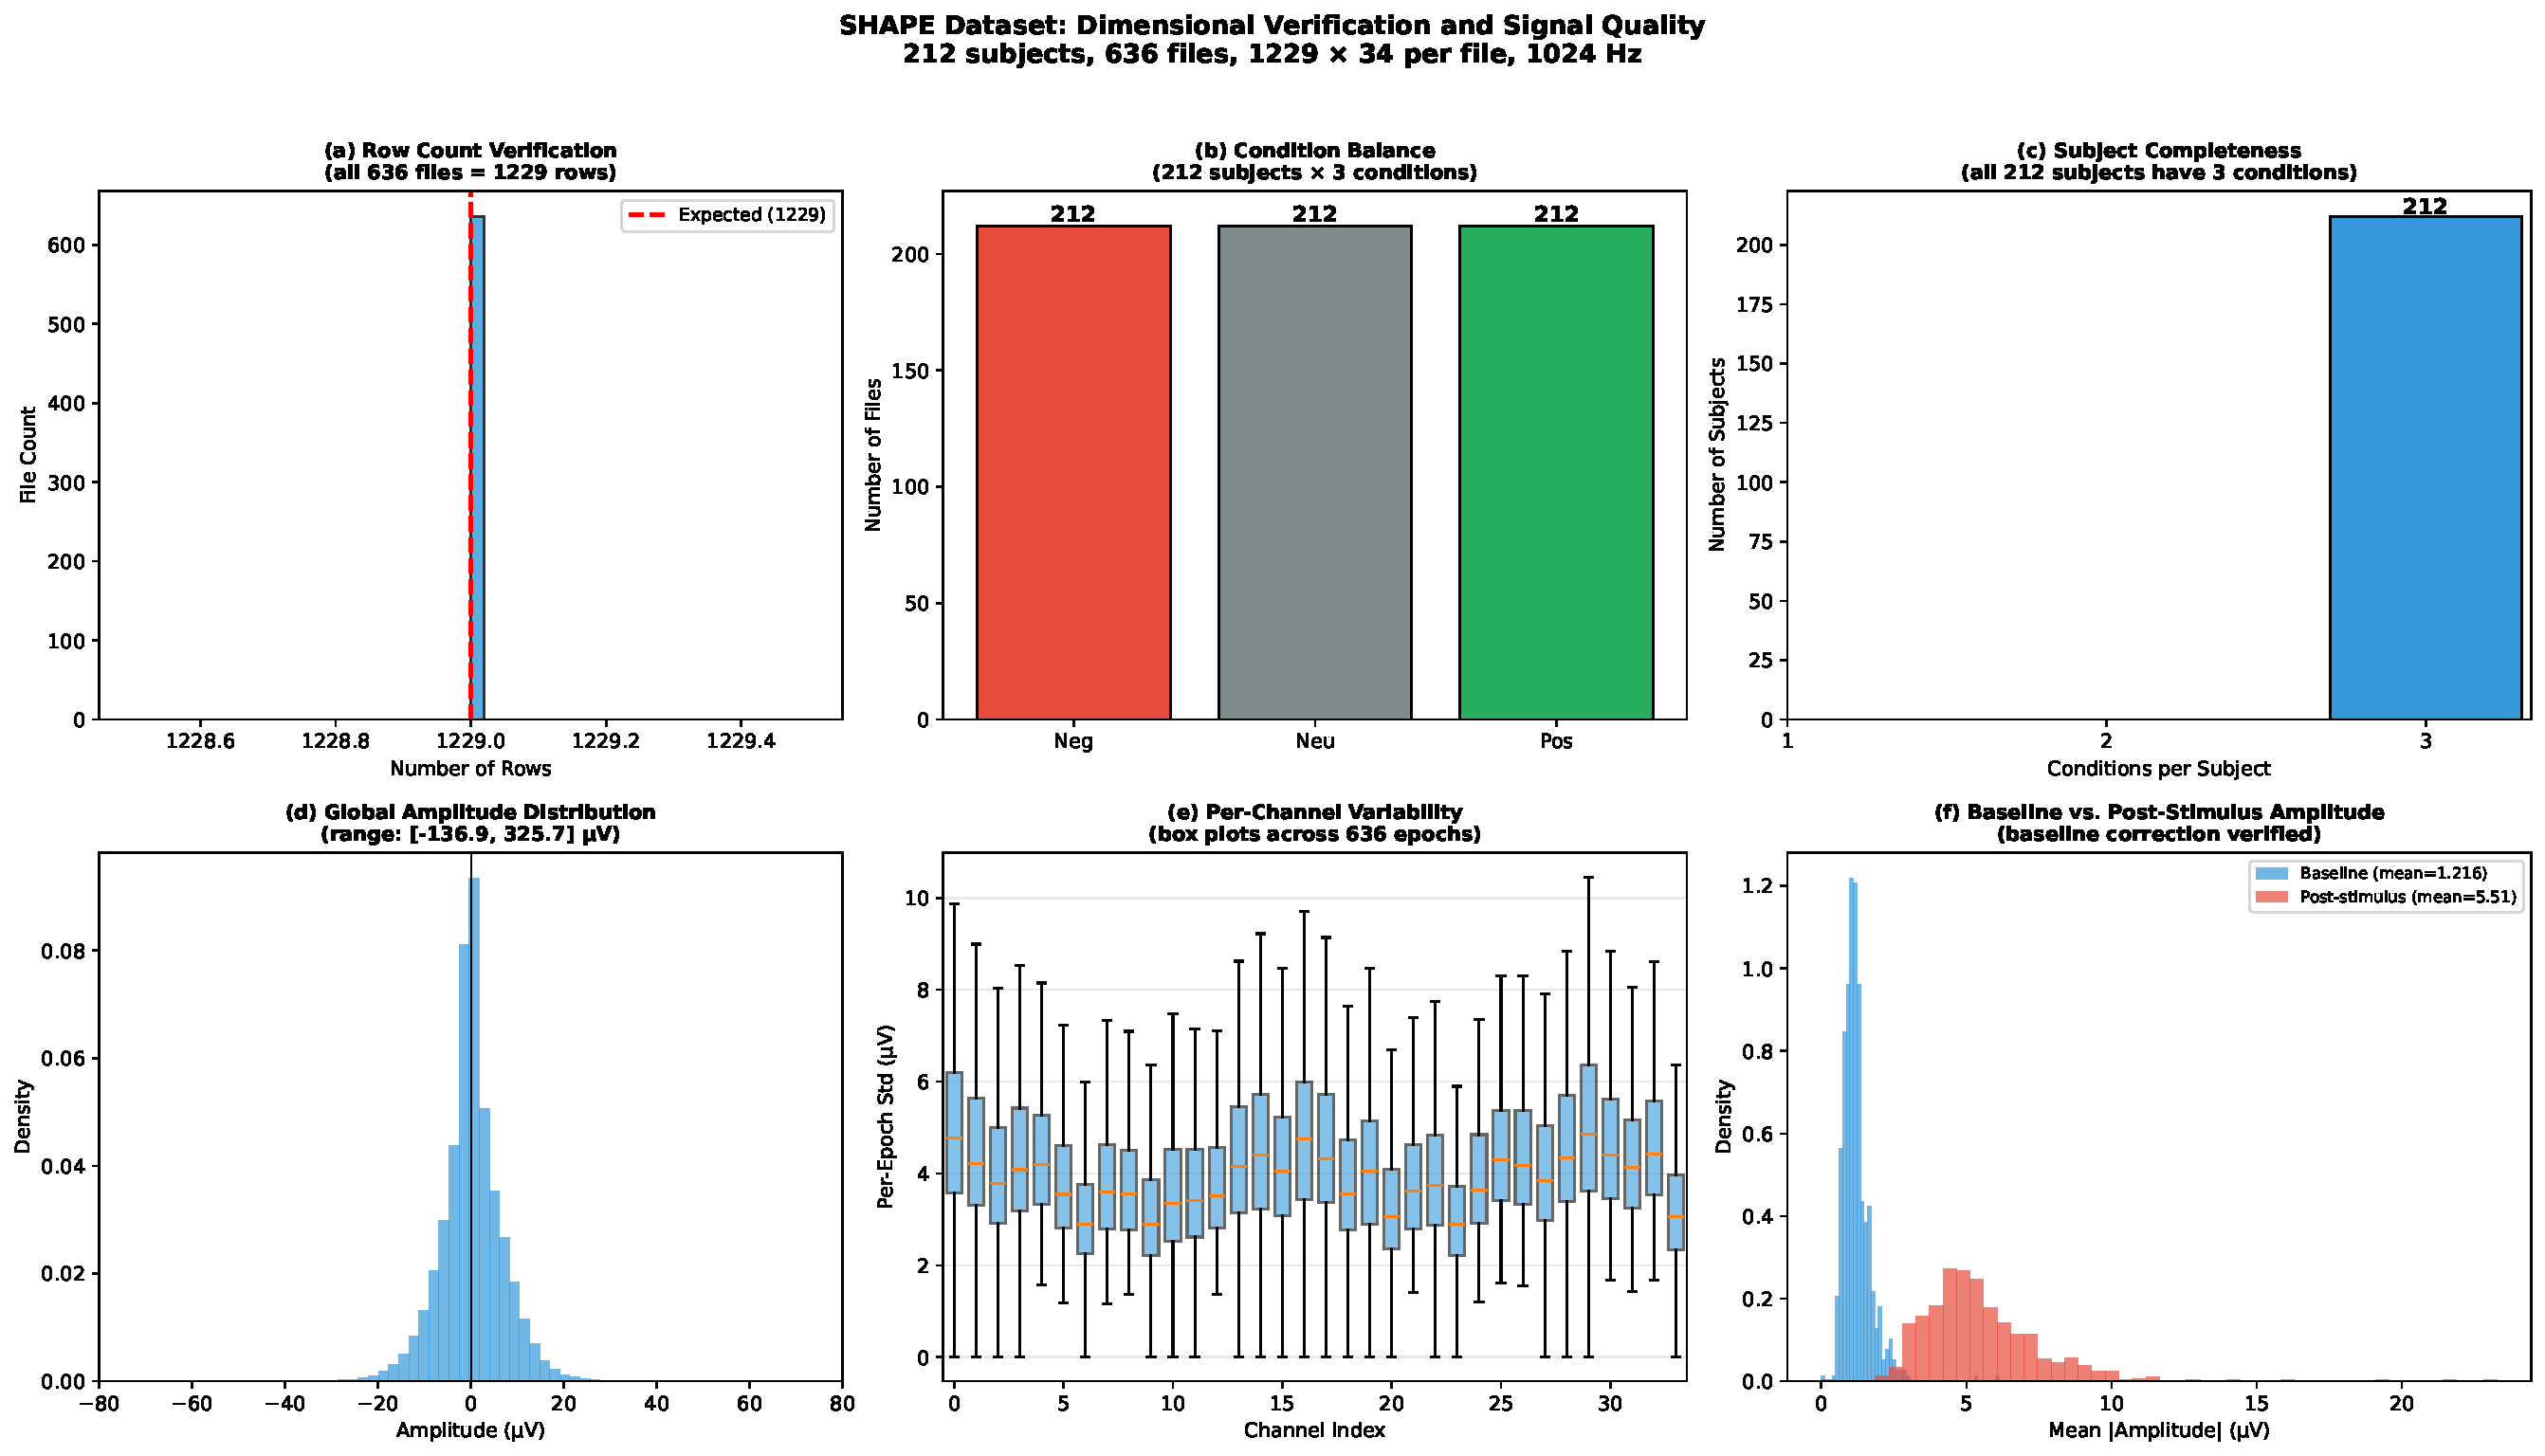
\includegraphics[width=\textwidth]{pictures/chGraphNeuralNetworks/fig_qc_dimensional_verification.pdf}
    \caption{Data verification across $636$ files. (a)~Row counts. (b)~Condition balance. (c)~Subject completeness. (d)~Global amplitude distribution. (e)~Per-channel variability. (f)~Baseline vs.\ post-stimulus amplitude.}
    \label{fig:qc_verification}
\end{figure}

\begin{figure}[H]
    \centering
    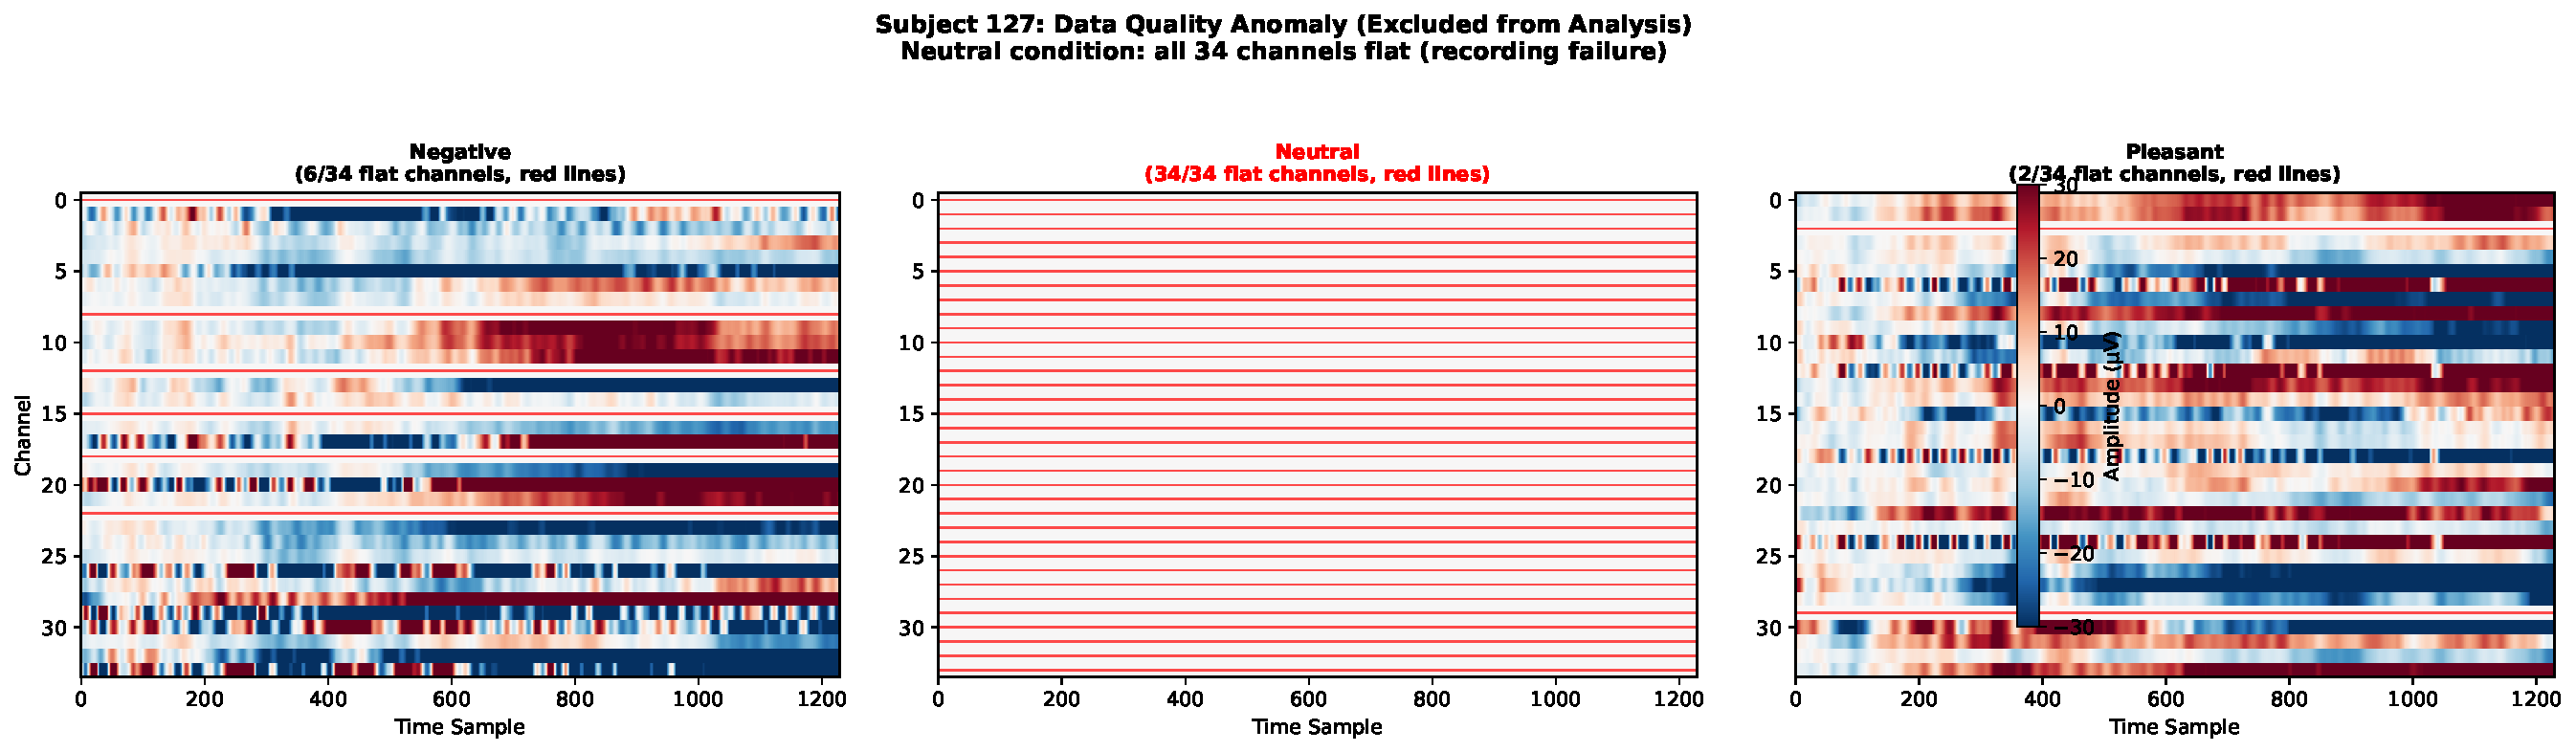
\includegraphics[width=\textwidth]{pictures/chGraphNeuralNetworks/fig_qc_subject127_anomaly.pdf}
    \caption{Subject~$127$ recording anomaly. The Neutral condition is entirely flat across all $34$ channels. Red lines indicate flat channels. This subject was excluded from all analyses.}
    \label{fig:qc_subject127}
\end{figure}

The final dataset comprises $\mathbf{211}$ \textbf{subjects} $\times$ $\mathbf{3}$ \textbf{conditions} $= \mathbf{633}$ \textbf{observations}.

\subsection{Clinical Metadata}

All $211$ subjects have comprehensive diagnostic metadata from structured clinical interviews (Figure~\ref{fig:clinical_profile}): $142$ with Major Depressive Disorder ($67.3\%$), $82$ with PTSD ($38.9\%$), $85$ with Substance Use Disorder ($40.3\%$), $60$ with GAD ($28.4\%$), $50$ with ADHD ($23.7\%$), $69$ with eating disorders ($32.7\%$), $34$ with mania ($16.1\%$), and $91$ on psychiatric medication ($43.1\%$). Biological sex: $172$ female, $33$ male. Mean comorbidity burden is $2.8$ diagnoses per subject (range $0$--$7$).

\begin{figure}[H]
    \centering
    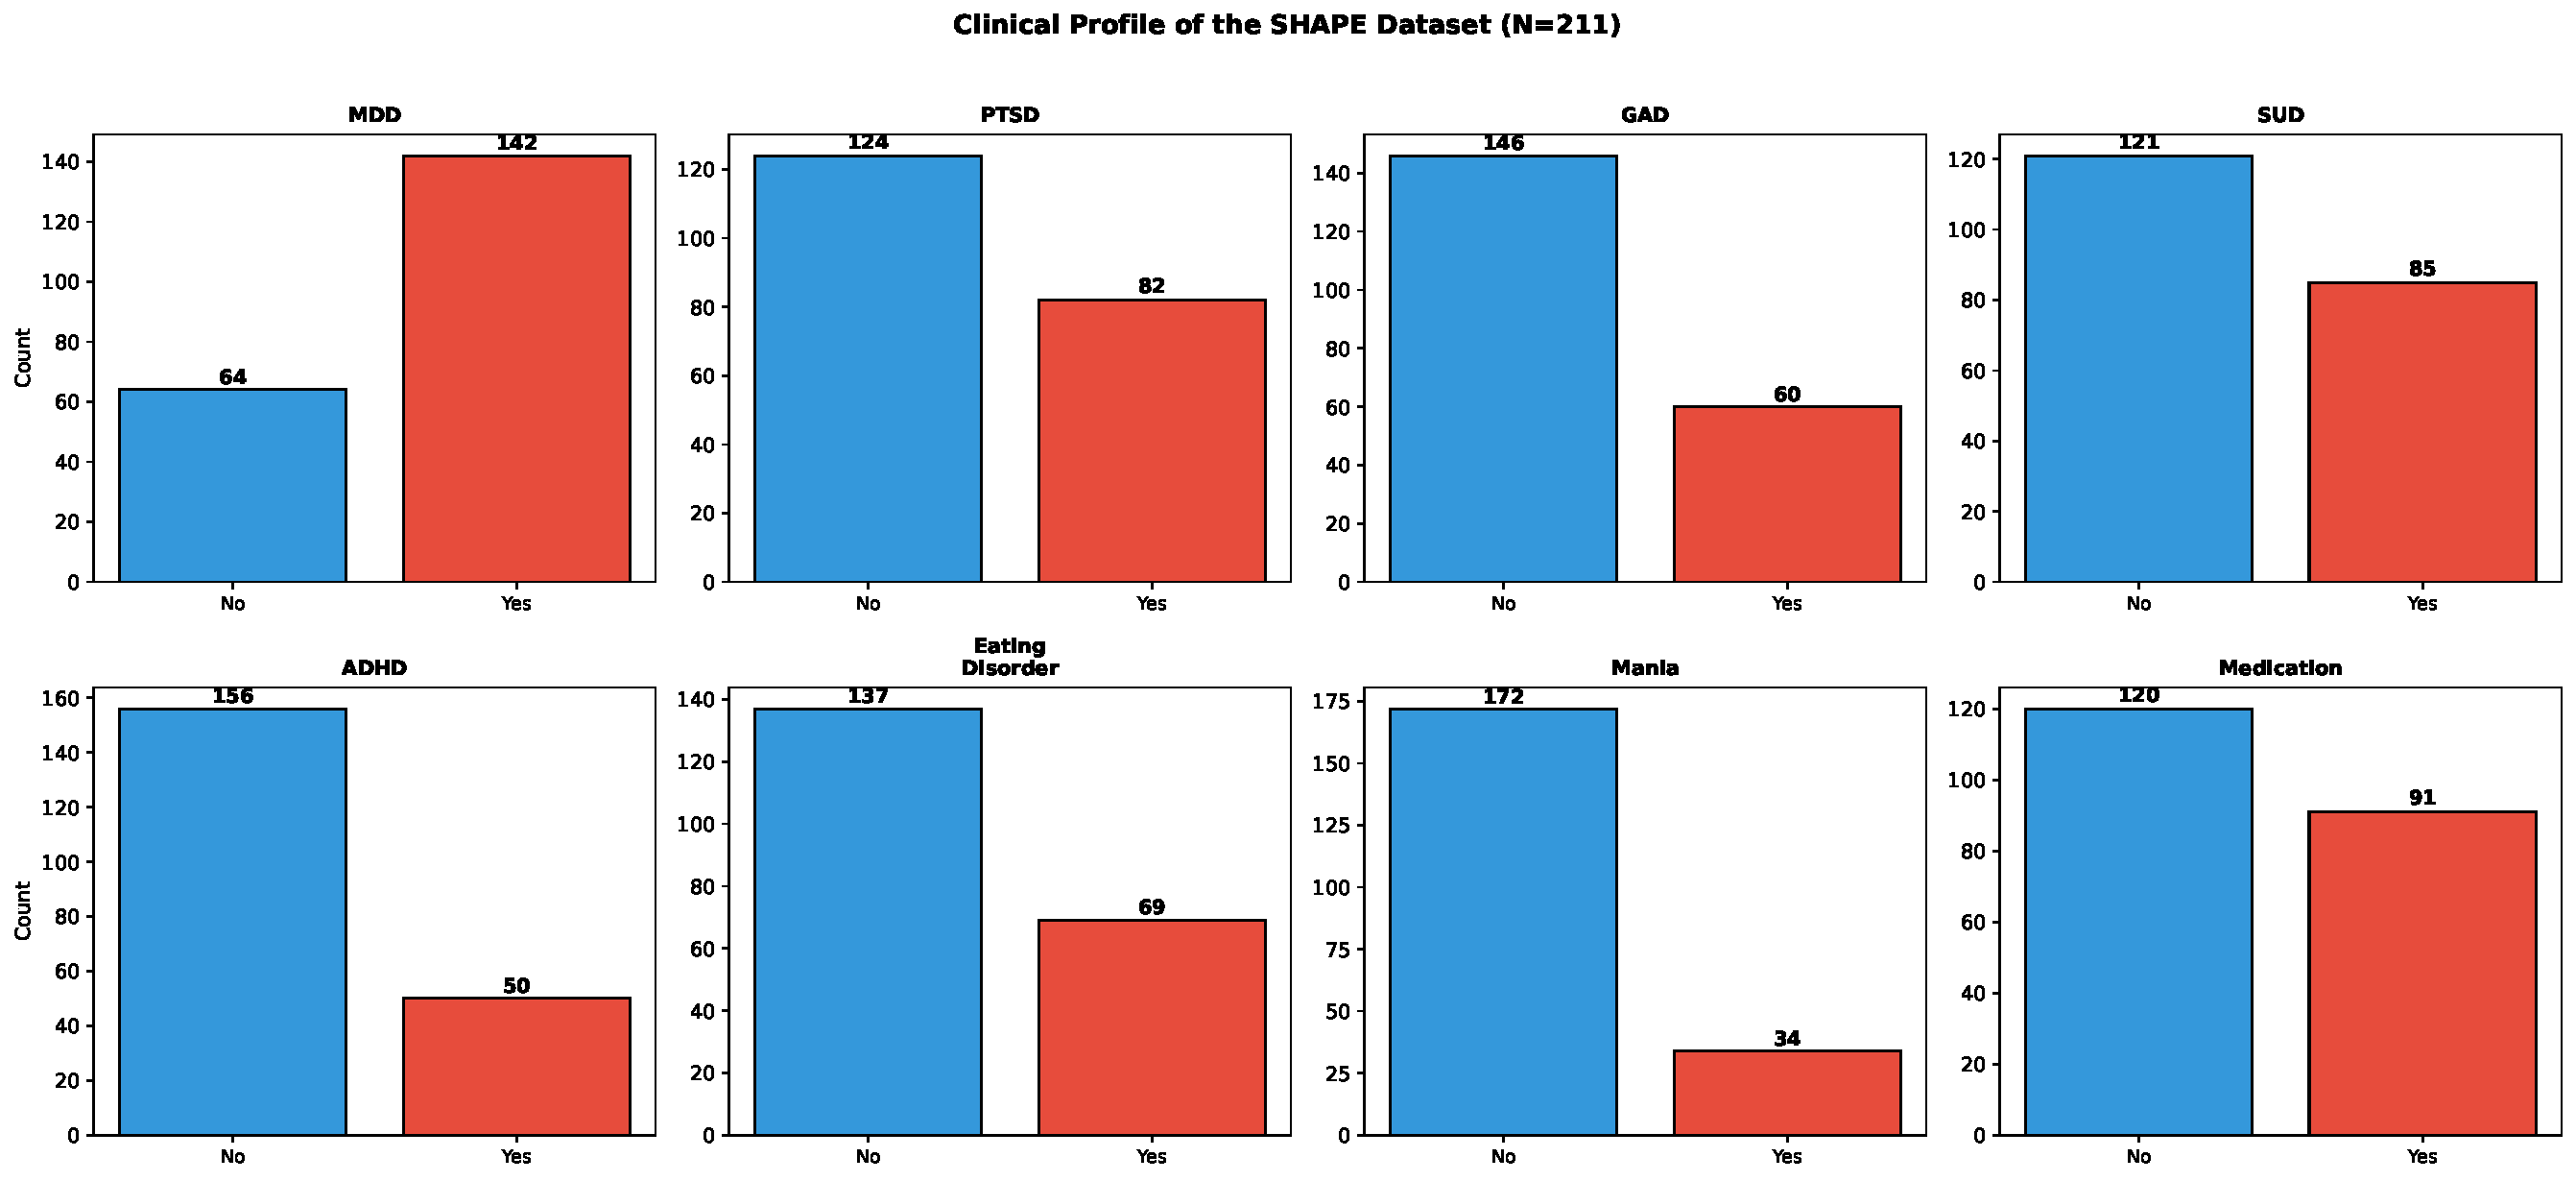
\includegraphics[width=\textwidth]{pictures/chGraphNeuralNetworks/fig_clinical_profile_211.pdf}
    \caption{Clinical profile of the $211$ SHAPE subjects. Eight diagnostic variables with group sizes.}
    \label{fig:clinical_profile}
\end{figure}

\subsection{Preprocessing Pipeline}

Four steps transform each raw $1229 \times 34$ ERP matrix into the reservoir format: baseline removal (discard first $205$ rows), $4\times$ anti-aliasing decimation to $256$~Hz ($256$ samples), per-channel z-score normalization, and LIF reservoir processing ($N_{\text{res}} = 256$, $\beta = 0.05$, $M_{\text{th}} = 0.5$) with BSC$_6$ encoding and PCA-64 reduction. The output is a $34 \times 64$ node feature matrix per observation.


\section{Raw Data Observations}
\label{sec:ch5_raw_obs}

Before classification and clinical analysis, this section characterizes the data at every stage of the graph pipeline: the z-scored multichannel EEG, the reservoir's spike response on real signals, the PCA-64 embedding geometry, the inter-channel connectivity structure, and the between-subject graph variability. These observations reveal several features of the data that constrain and inform all downstream analyses.

\subsection{Multichannel EEG Entering the Graph Stage}

The preprocessed dataset provides $633$ epochs ($211$ subjects $\times$ $3$ conditions), each a $256 \times 34$ matrix of z-scored amplitudes at $256$~Hz. Figure~\ref{fig:obs01_eeg} displays representative epochs for three subjects spanning the clinical spectrum. After per-channel z-scoring, the global distribution is centered at $0.000$ with unit variance and a range of $[-5.41, 5.01]$. Visual inspection reveals substantial inter-subject variability in waveform morphology: the temporal structure of the multichannel response differs markedly across subjects, even within the same emotional condition. This variability is the dominant signal in the data and explains why subject-level cross-validation is essential.

\begin{figure}[H]
    \centering
    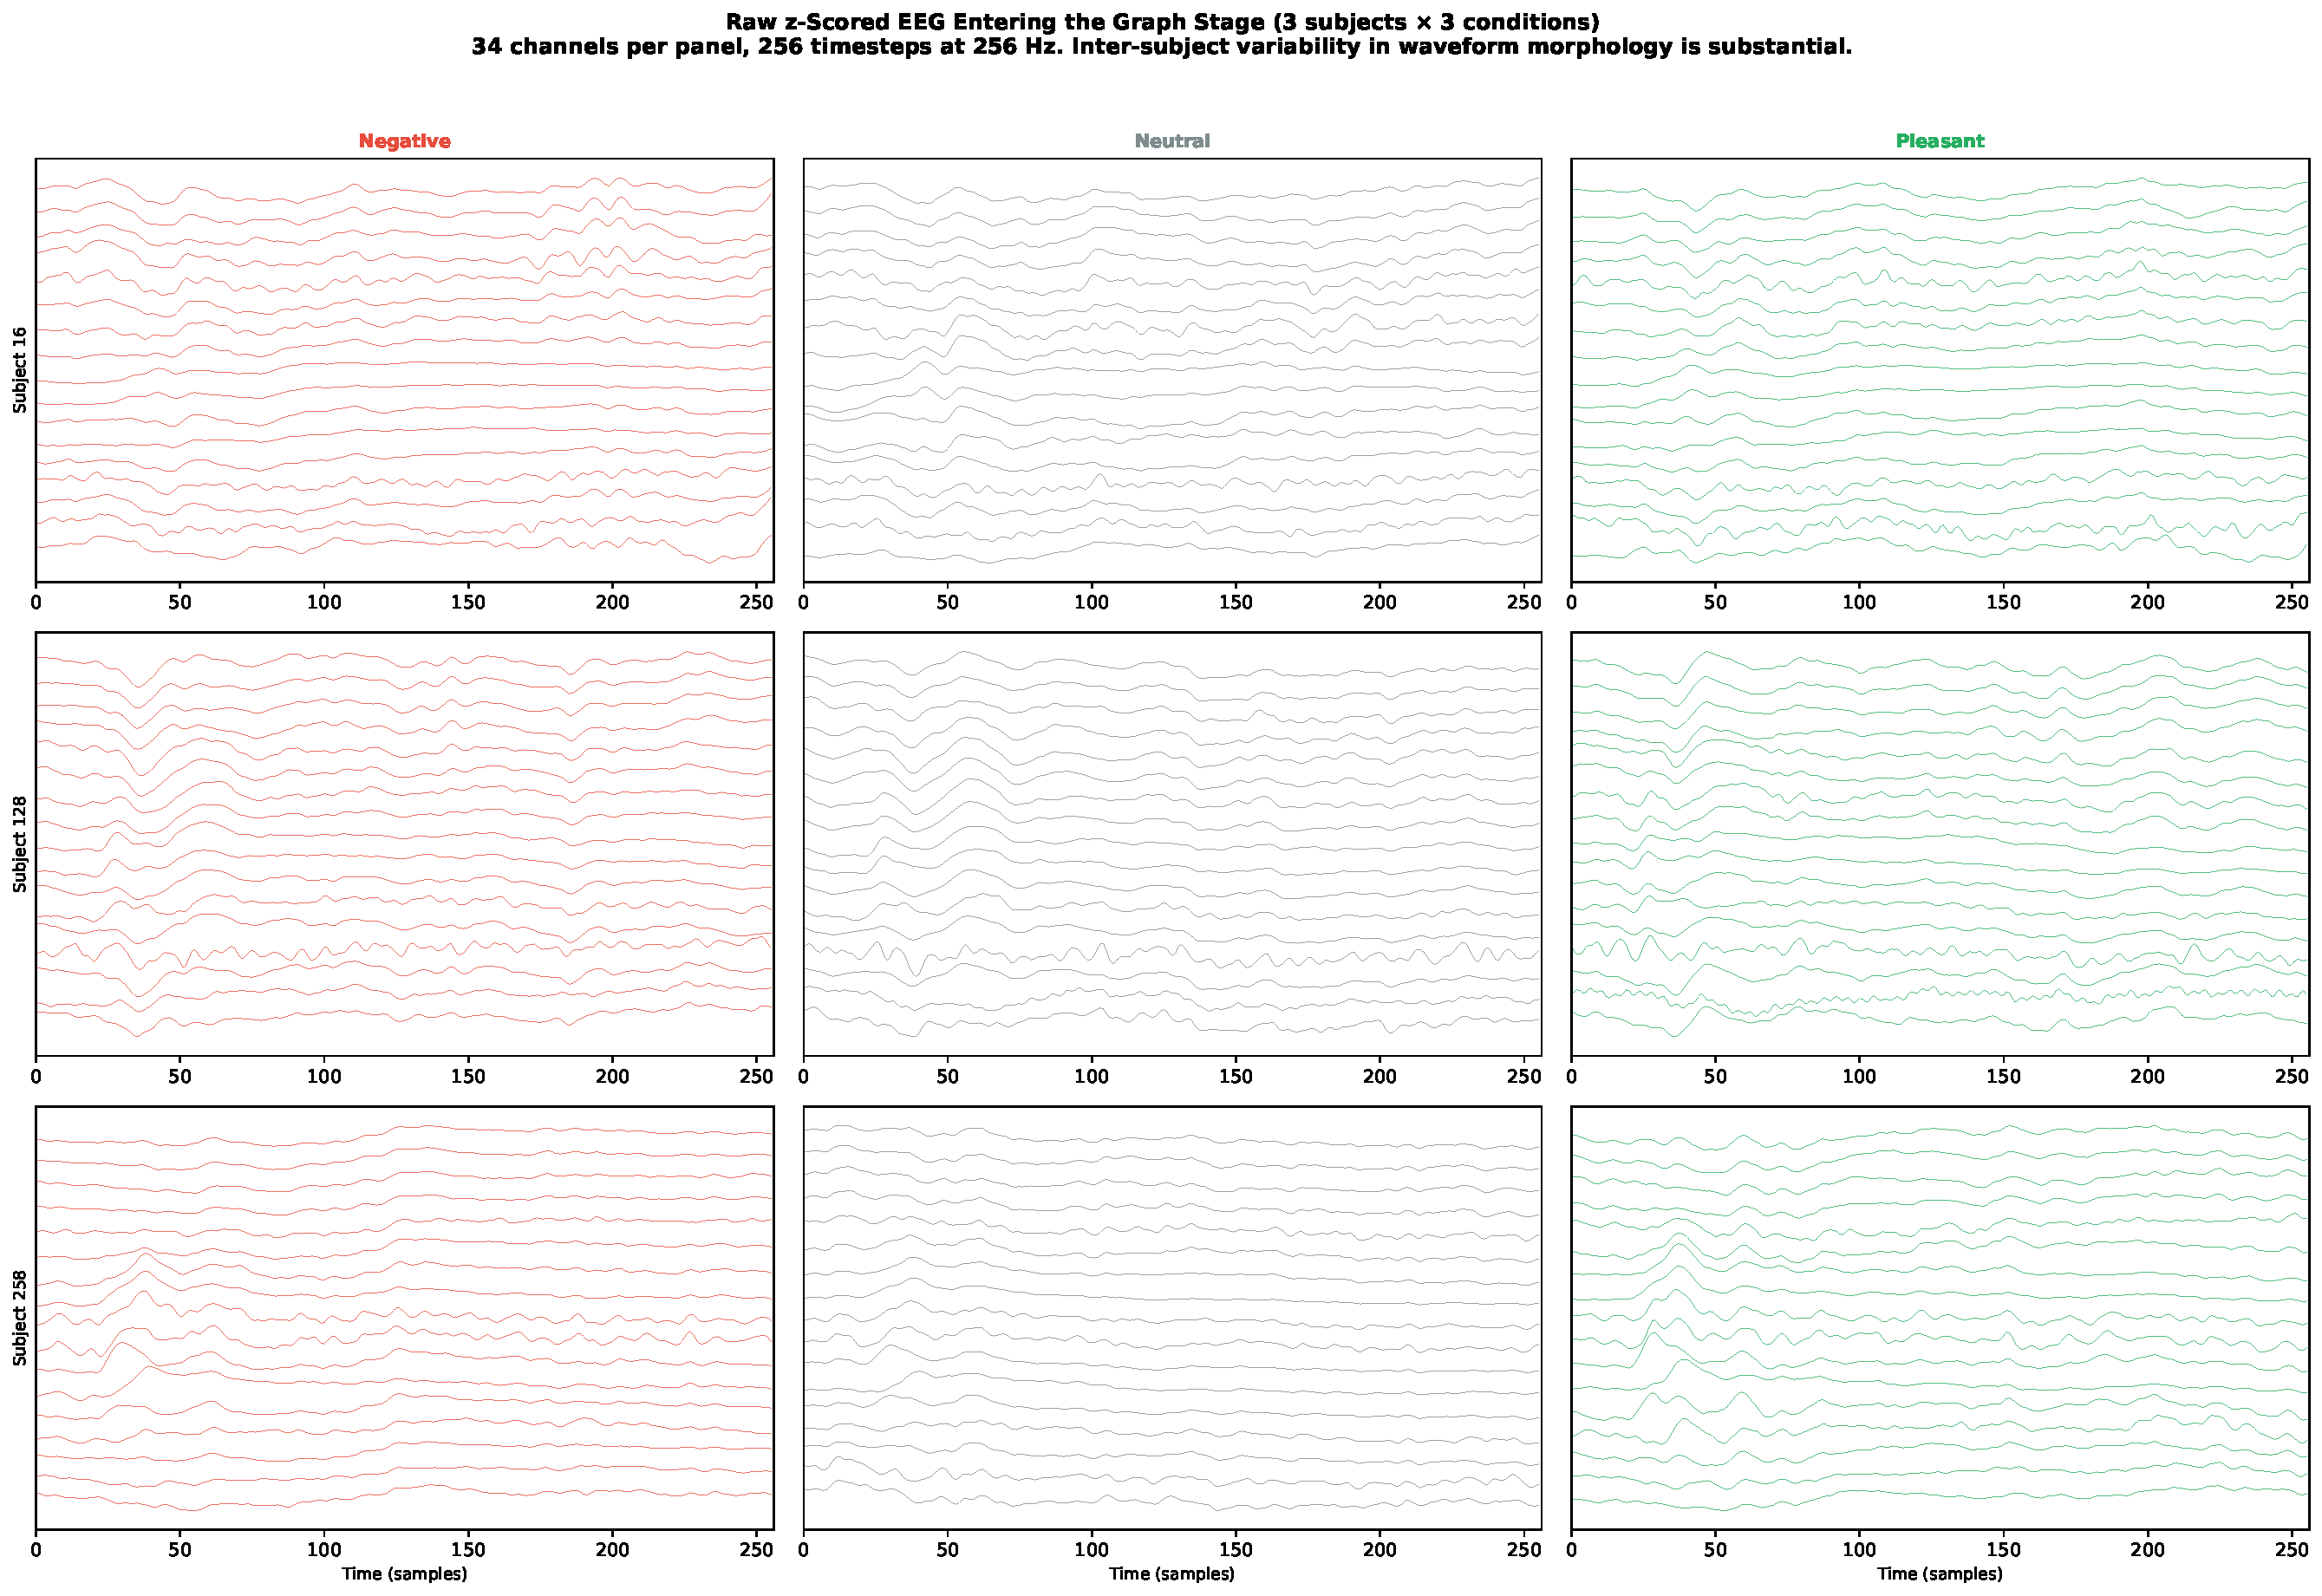
\includegraphics[width=\textwidth]{pictures/chGraphNeuralNetworks/obs01_raw_eeg_waveforms.pdf}
    \caption{Raw z-scored EEG entering the graph stage ($3$ subjects $\times$ $3$ conditions). Each panel shows $17$ of $34$ channels offset vertically, $256$ timesteps. Inter-subject waveform variability is substantially larger than between-condition differences within each subject.}
    \label{fig:obs01_eeg}
\end{figure}

\subsection{Reservoir Spike Response on Real EEG}

Figure~\ref{fig:obs02_spikes} shows the LIF reservoir's response to real SHAPE EEG for a representative subject across all three conditions. The top row displays spike rasters for a single channel (Channel~10): the reservoir transforms the continuous z-scored input into sparse binary spike trains whose temporal density tracks the input amplitude envelope. The bottom row shows population firing rate traces for four channels, revealing that different channels produce different temporal activation profiles---the inter-channel heterogeneity that the graph analysis will exploit. The BSC$_6$ features extracted from these spike trains have $47.4\%$ zero entries (compared to $79.1\%$ on the synthetic task), reflecting the richer and more sustained drive from real EEG relative to the brief synthetic pulses. Mean BSC$_6$ feature value is $5.15$ with a maximum of $42$ spikes per neuron per bin.

\begin{figure}[H]
    \centering
    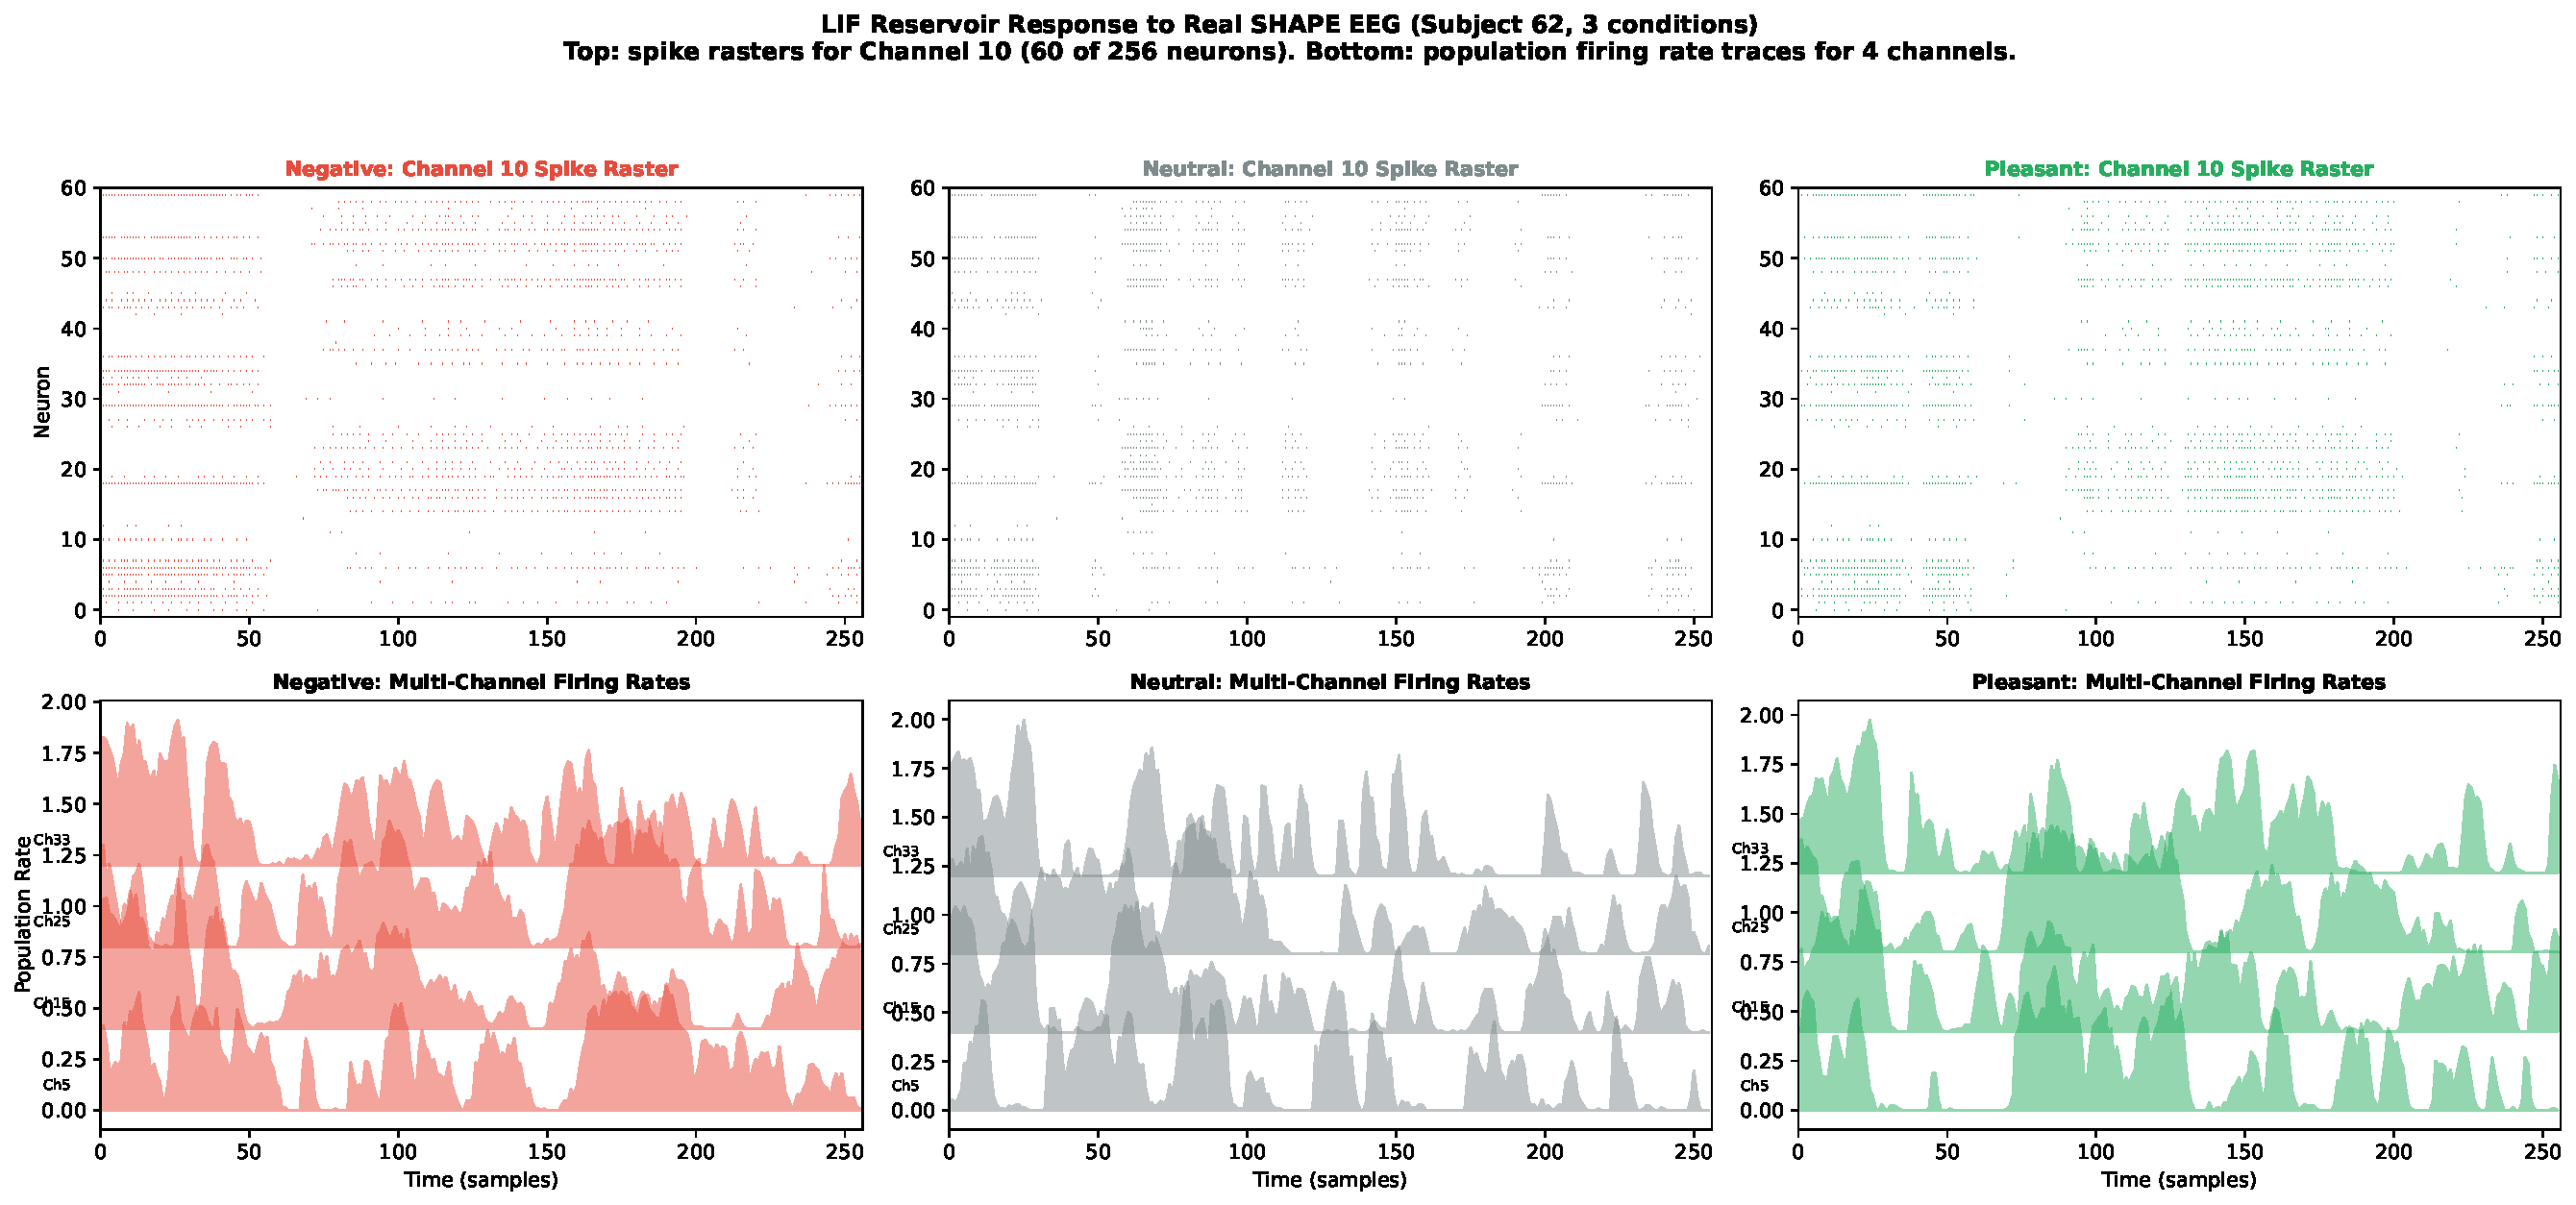
\includegraphics[width=\textwidth]{pictures/chGraphNeuralNetworks/obs02_raw_spike_trains.pdf}
    \caption{LIF reservoir response to real SHAPE EEG (one subject, three conditions). Top: spike rasters for Channel~10 ($60$ of $256$ neurons). Bottom: population firing rate traces for four channels. Different channels produce different temporal activation profiles, providing the inter-channel heterogeneity that graph analysis exploits.}
    \label{fig:obs02_spikes}
\end{figure}

\subsection{PCA-64 Embedding Geometry}

Figure~\ref{fig:obs03_embeddings} characterizes the PCA-64 embedding space. The left panel projects the concatenated $34 \times 64 = 2{,}176$-dimensional embeddings into two dimensions, colored by emotional condition. The three conditions overlap substantially---there is no clean geometric separation visible in two dimensions, consistent with the moderate classification accuracy ($63.4\%$) rather than near-perfect separation. The center panel colors the same projection by subject identity, revealing that subject-level clustering dominates: observations from the same subject cluster tightly regardless of condition. This confirms that between-subject variability ($\sigma_{\text{edge}} = 0.303$) is far larger than the condition-dependent signal ($|\Delta r| = 0.045$). The right panel shows per-channel embedding variance, which ranges from $36{,}900$ (Channel~16) to $70{,}721$ (Channel~29) with a coefficient of variation of $0.15$. This $1.9\times$ range indicates moderate heterogeneity: some channels carry more total variance than others, though all channels are active.

\begin{figure}[H]
    \centering
    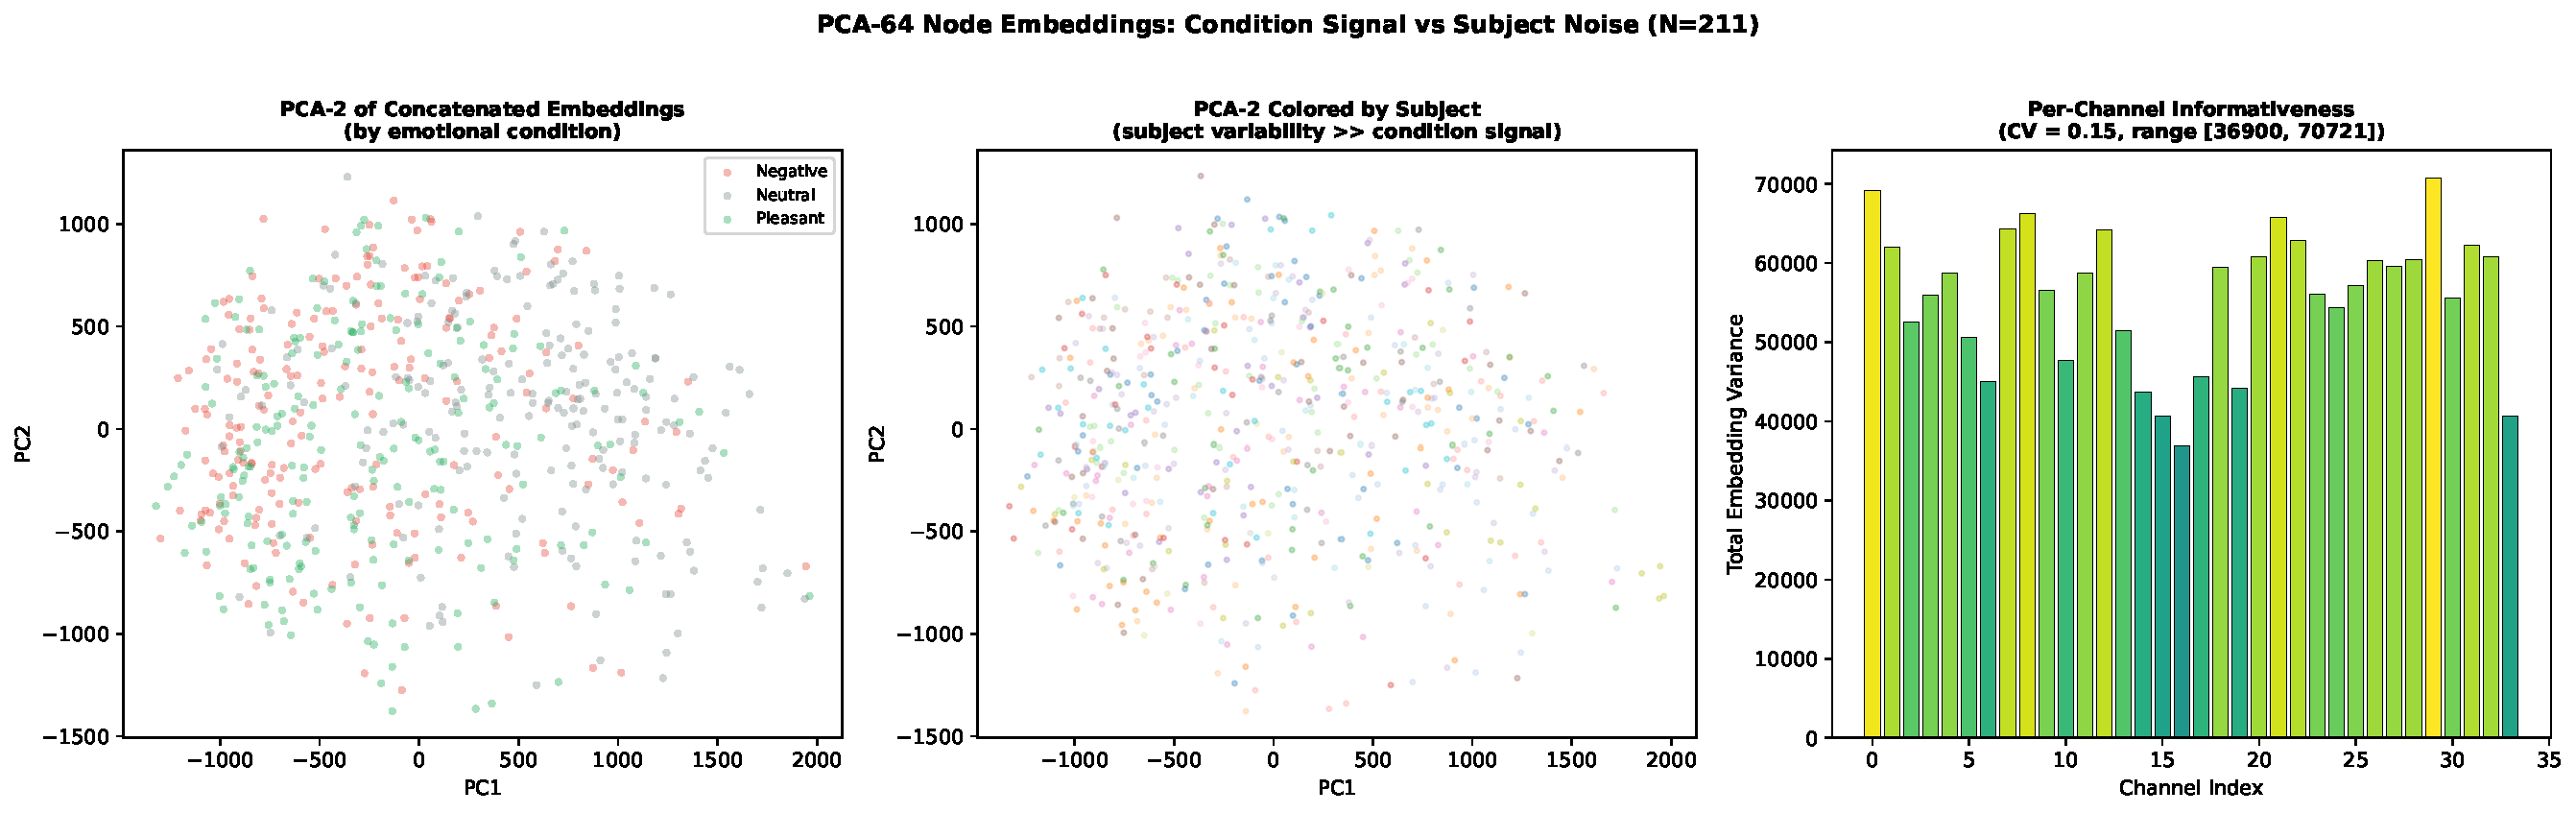
\includegraphics[width=\textwidth]{pictures/chGraphNeuralNetworks/obs03_bsc6_pca64_embeddings.pdf}
    \caption{PCA-64 embedding geometry ($N = 211$). Left: PCA-2 by condition (substantial overlap). Center: PCA-2 by subject (subject clustering dominates). Right: per-channel embedding variance (CV $= 0.15$, range $1.9\times$). Subject variability is the dominant source of variance in the embedding space.}
    \label{fig:obs03_embeddings}
\end{figure}

\subsection{Inter-Channel Connectivity and Graph Topology}

Figure~\ref{fig:obs04_connectivity} displays the inter-channel correlation matrices and their corresponding graph topologies for each condition. The mean Pearson correlation across all observations is $\bar{r} = 0.143$ with standard deviation $0.552$, indicating broad and heterogeneous inter-channel relationships: $34.8\%$ of channel pairs have correlation exceeding $0.5$, while $40.8\%$ are negative. The correlation structure is condition-dependent but the differences are subtle: mean $r$ is $0.147$, $0.145$, and $0.138$ for Negative, Neutral, and Pleasant respectively.

At the $20\%$ density threshold, each condition-average graph contains $113$ edges with mean degree $6.6$ and maximum degree $13$. The graphs (Figure~\ref{fig:obs04_connectivity}, bottom row) show that the topology is not uniform: some channels are hubs (degree $> 10$) while others are peripheral (degree $= 1$--$2$). The mean clustering coefficient is $0.804$, indicating high local redundancy---neighbors of a node tend to be neighbors of each other. The thresholded correlation values range from $r = 0.506$ (Pleasant) to $r = 0.545$ (Negative), meaning only strongly correlated pairs are retained as edges.

\begin{figure}[H]
    \centering
    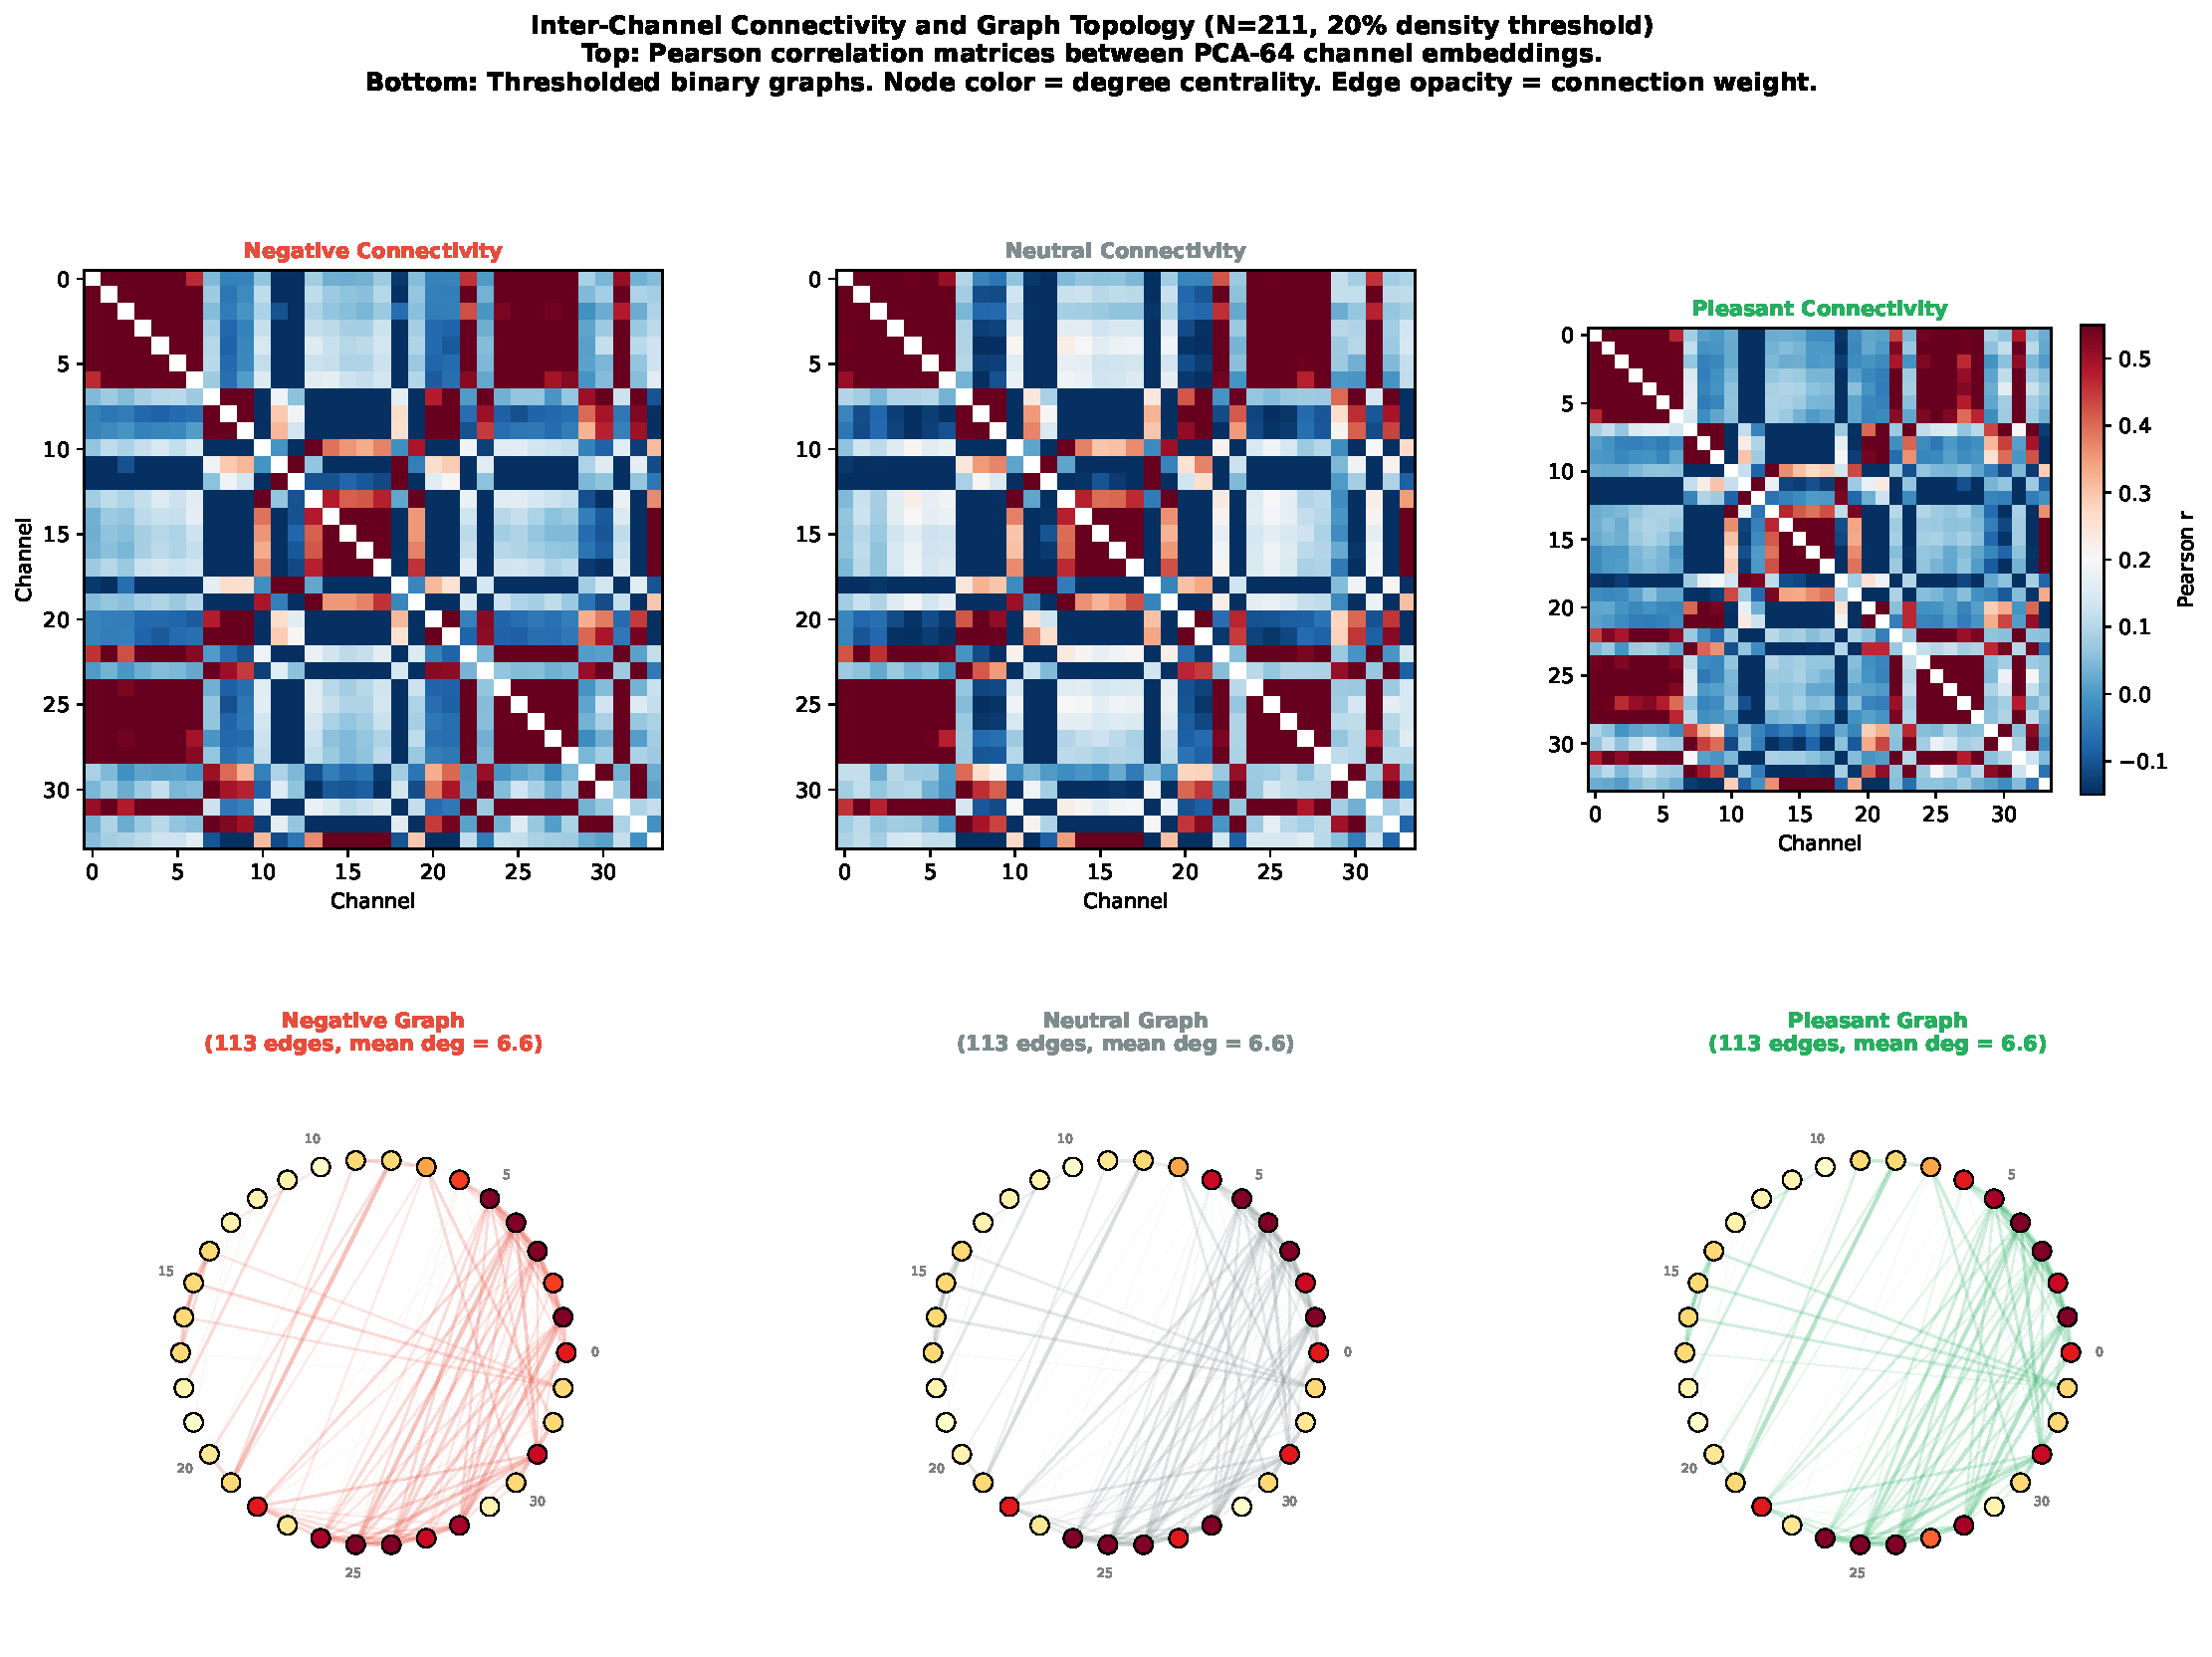
\includegraphics[width=\textwidth]{pictures/chGraphNeuralNetworks/obs04_raw_connectivity_matrices.pdf}
    \caption{Inter-channel connectivity and graph topology ($N = 211$, $20\%$ density). Top: Pearson correlation matrices (mean $\bar{r} = 0.143$, $34.8\%$ of pairs $> 0.5$, $40.8\%$ negative). Bottom: thresholded graphs with $113$ edges each. Node color $=$ degree centrality; edge opacity $\propto$ connection weight. Hub and peripheral channels are visible.}
    \label{fig:obs04_connectivity}
\end{figure}

\subsection{Between-Subject Graph Variability}

Figure~\ref{fig:obs07_variability} quantifies the between-subject variability in graph structure. Individual subject graphs (top row) show substantial topological diversity: the same $20\%$ density threshold produces different hub locations, different edge patterns, and different degree distributions across subjects. The bottom-left panel shows that edge-level variability ($\sigma = 0.303$) spans the full range of edge weights, with stronger edges being more variable. The degree distribution across all subjects and channels (bottom center) is unimodal with a mean of $6.6$ and a range from $0$ to $15$.

The condition-difference graph (bottom right, Negative minus Pleasant) reveals which channel pairs show the largest emotional modulation. The signal-to-noise comparison (far right) quantifies the fundamental challenge: between-subject edge variability ($\sigma = 0.303$) is $7\times$ larger than the mean condition-dependent signal ($|\Delta r| = 0.045$). This ratio constrains every analysis in this chapter: the condition signal is real but weak relative to the dominant source of variance, which is inter-individual differences in brain network organization. Any classification or clinical analysis method must extract this weak signal from within strong subject-level noise.

\begin{figure}[H]
    \centering
    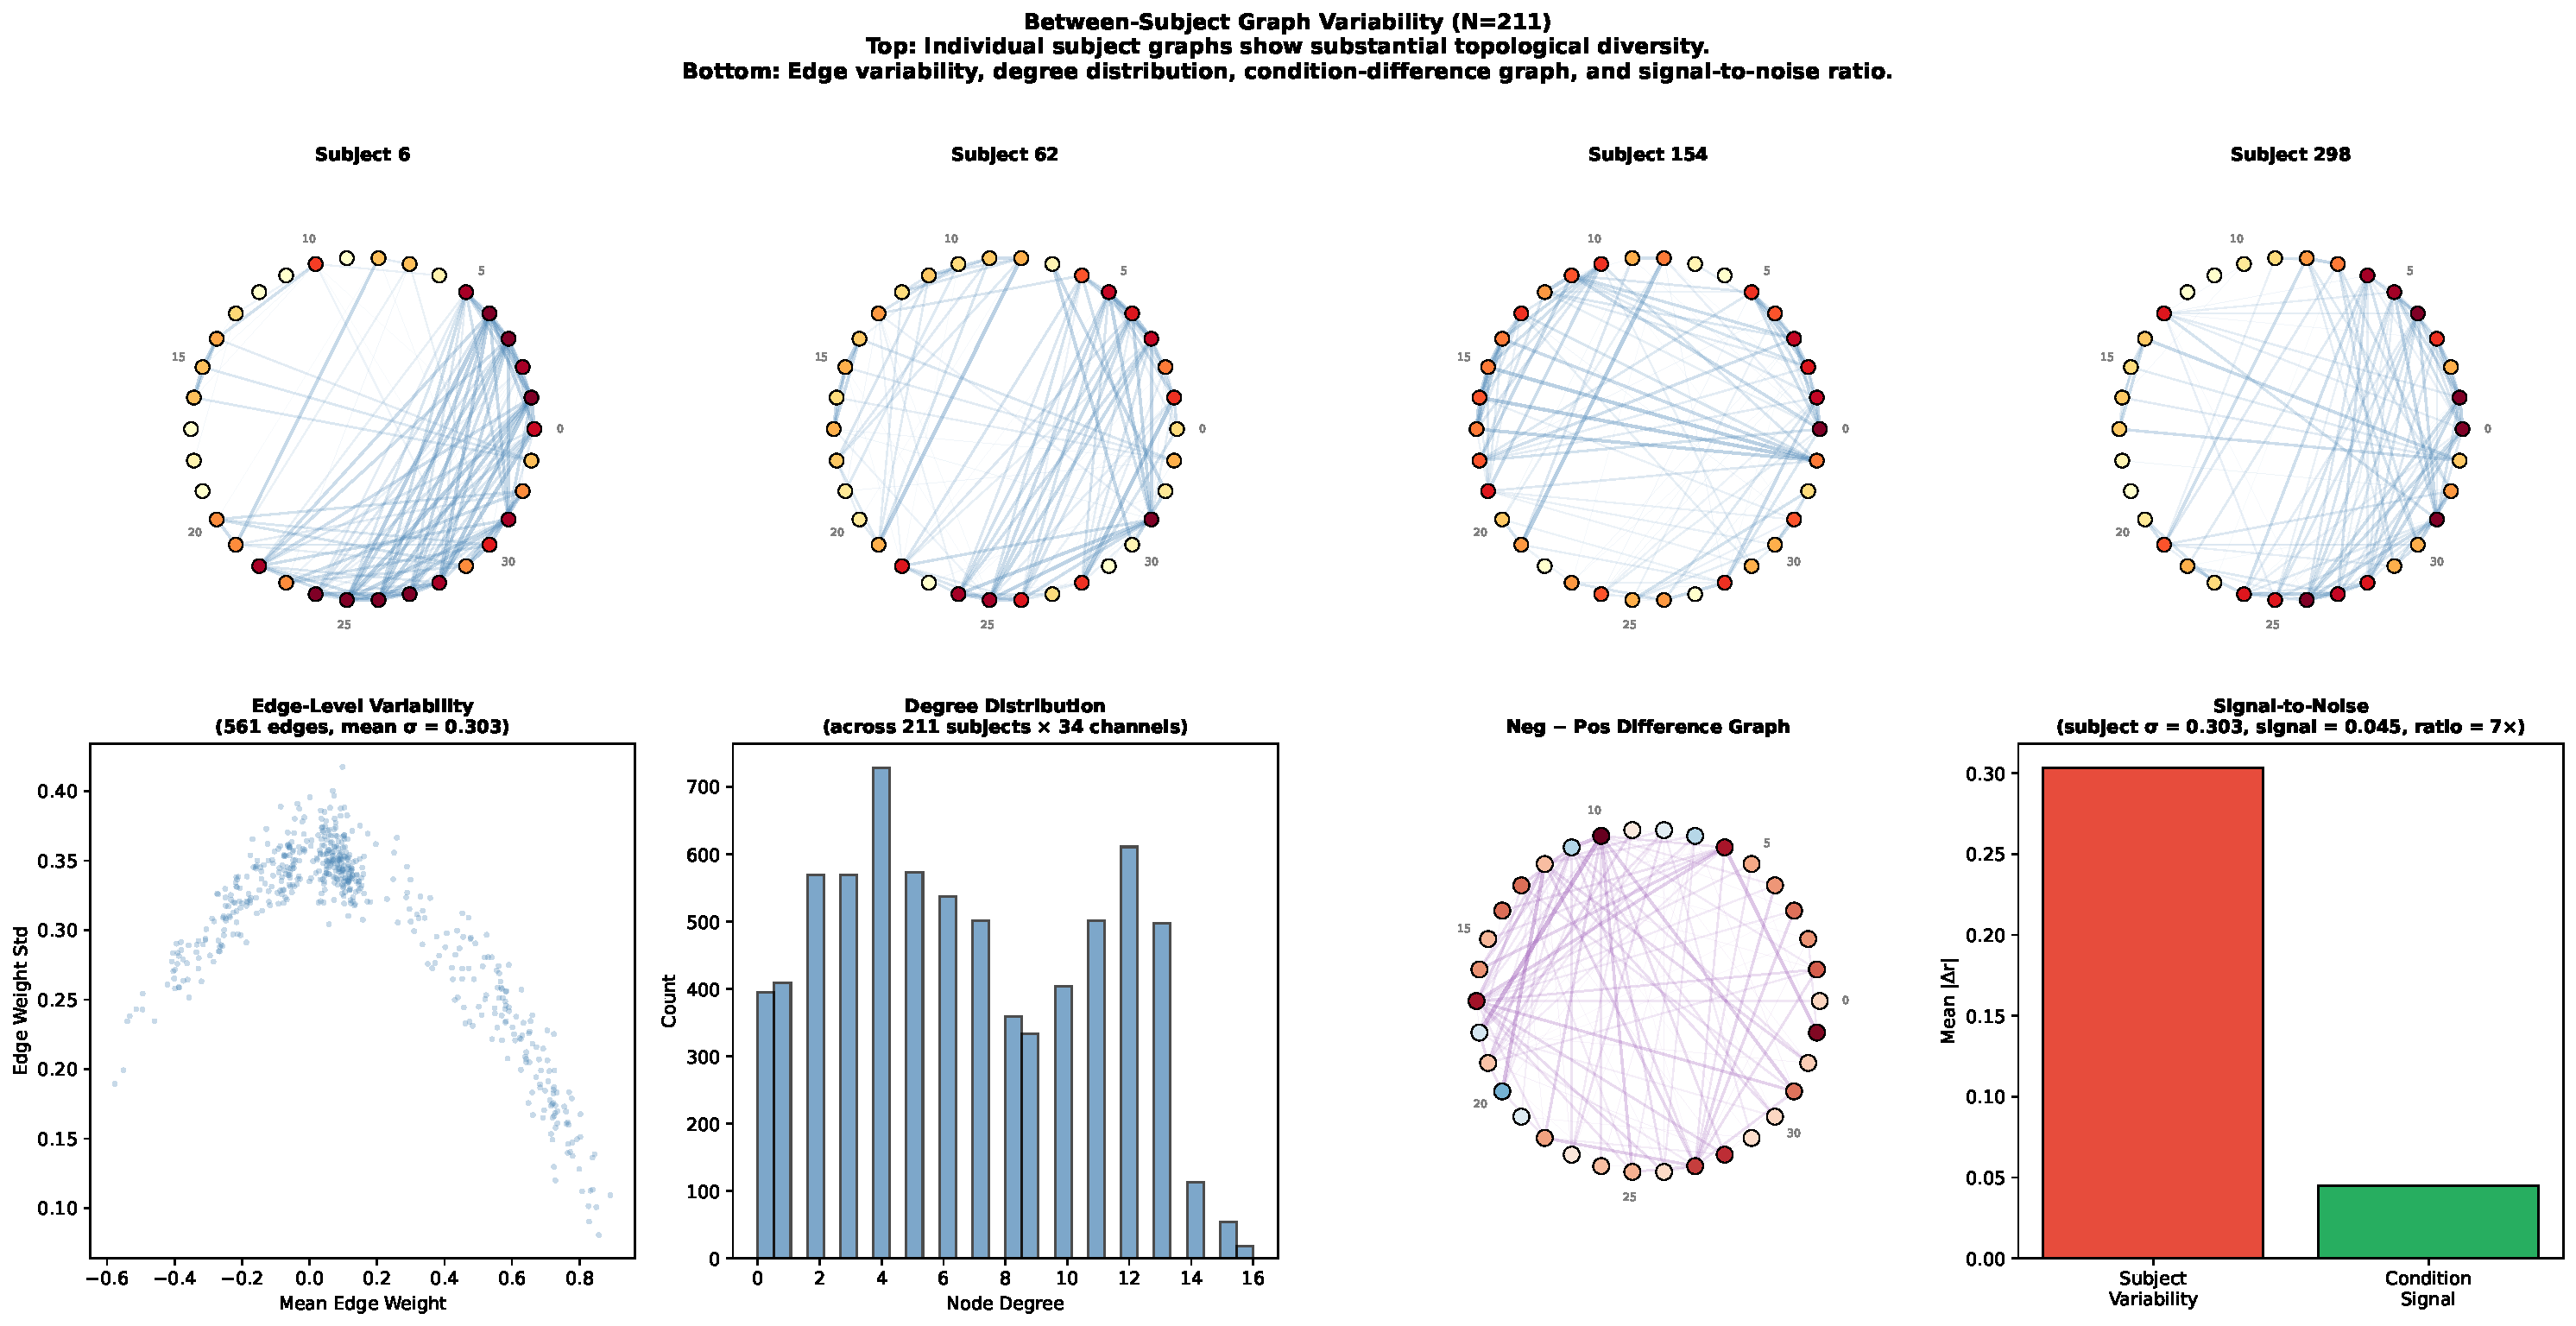
\includegraphics[width=\textwidth]{pictures/chGraphNeuralNetworks/obs07_graph_variability.pdf}
    \caption{Between-subject graph variability ($N = 211$). Top: four individual subject graphs showing topological diversity. Bottom: edge-level variability scatter ($\sigma = 0.303$), degree distribution across all subjects, condition-difference graph (Neg $-$ Pos), and signal-to-noise comparison ($7\times$ more subject noise than condition signal).}
    \label{fig:obs07_variability}
\end{figure}

These five observation subsections, with their associated figures and quantitative statistics, establish the data landscape. The key structural features are: (1)~subject variability dominates condition signal by $7\times$; (2)~the graph is small ($34$ nodes), dense ($20\%$, $113$ edges), and highly clustered ($\bar{C} = 0.804$); (3)~the embedding space shows moderate channel heterogeneity but no clean geometric separation by condition; and (4)~the correlation structure is broad, with $40.8\%$ negative pairs indicating genuine heterophily.

\subsection{The Reservoir's Spike Representation on Real EEG}

Figure~\ref{fig:obs13_bsc6} characterizes the BSC$_6$ feature structure that the reservoir produces from real clinical EEG---the representation that every subsequent analysis in this chapter operates on. Each observation is a $34 \times 256 \times 6$ tensor ($34$ channels, $256$ reservoir neurons, $6$ temporal bins), yielding $52{,}224$ spike-count features per observation. The representation is $47.4\%$ sparse (compared to $79.1\%$ on the synthetic task in Chapter~\ref{chap:embeddings}), reflecting the richer and more sustained drive from real EEG. Non-zero entries have a mean of $9.79$ and a median of $7$ spikes per neuron per bin, with a maximum of $42$.

\begin{figure}[H]
    \centering
    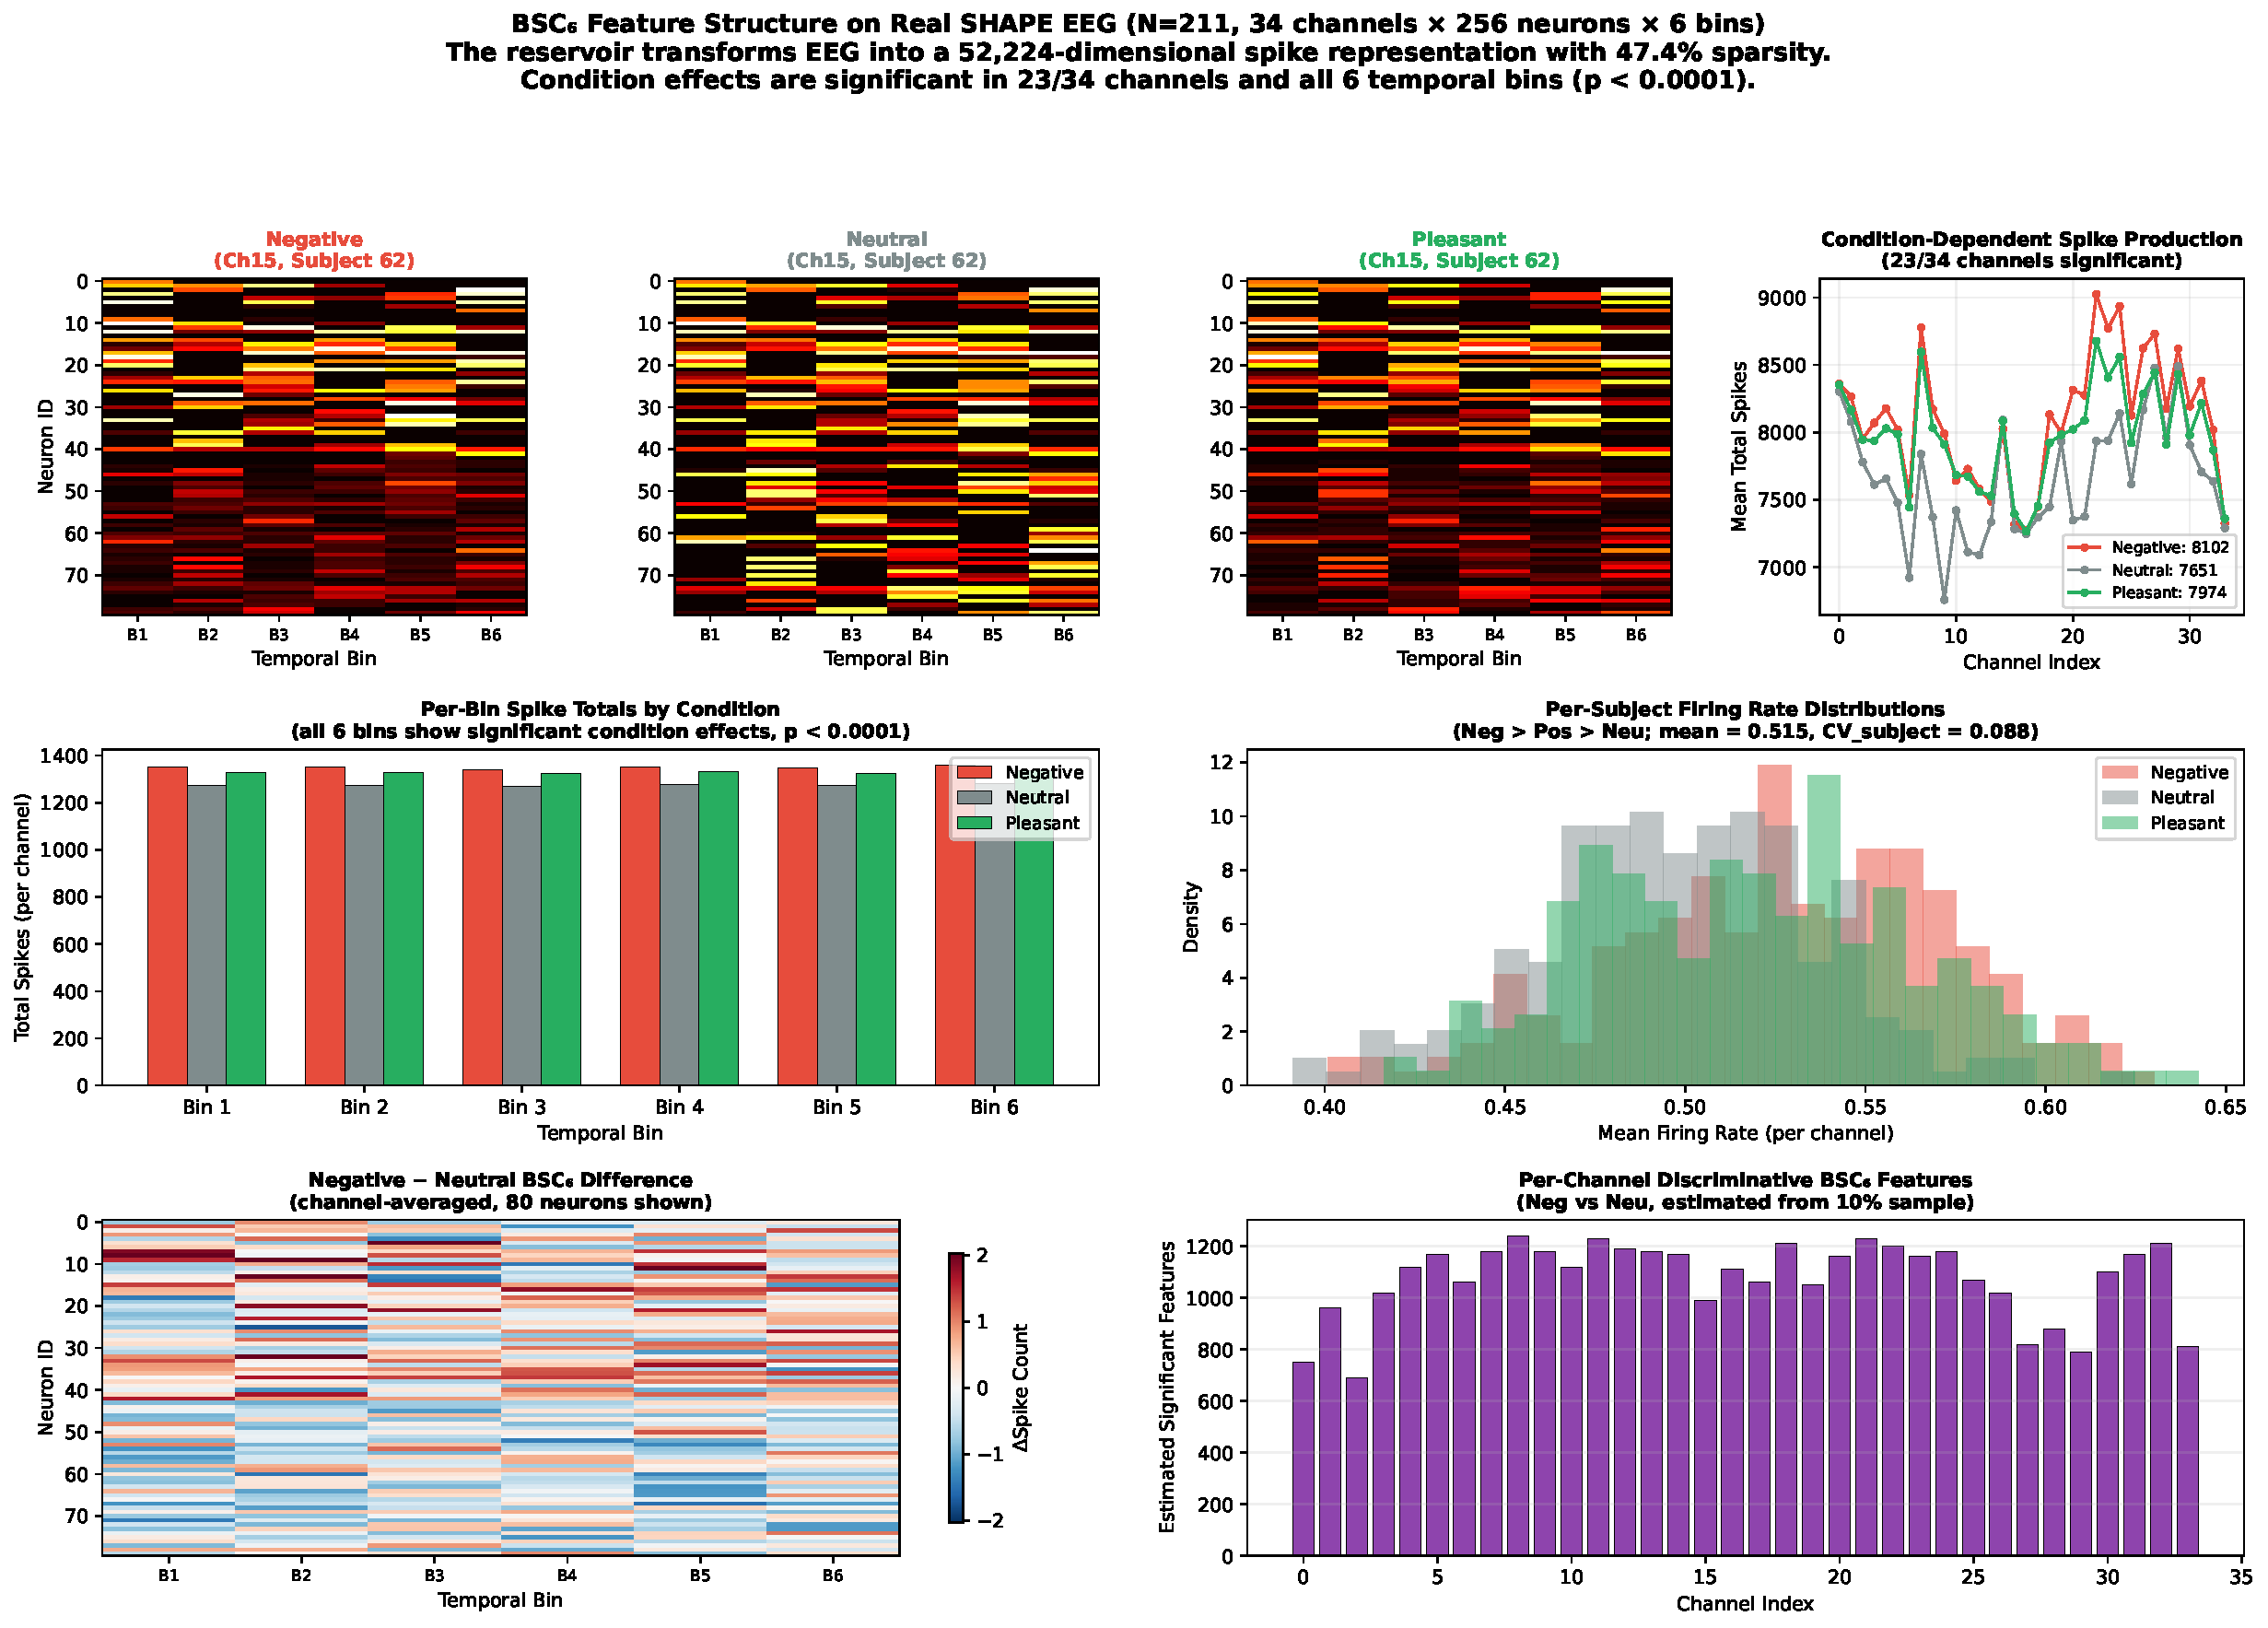
\includegraphics[width=\textwidth]{pictures/chGraphNeuralNetworks/obs13_bsc6_real_eeg.pdf}
    \caption{BSC$_6$ features on real SHAPE EEG ($N = 211$, $34$ channels $\times$ $256$ neurons $\times$ $6$ bins $= 52{,}224$ features per observation). Top: single-subject BSC$_6$ heatmaps by condition and condition-dependent spike production across channels ($23/34$ significant). Middle: per-bin spike totals by condition (all $6$ bins $p < 0.0001$) and per-subject firing rate distributions. Bottom: class-average difference map and per-channel discriminative feature counts.}
    \label{fig:obs13_bsc6}
\end{figure}

The condition structure in the spike representation is both distributed and highly significant. The Negative condition produces $8{,}102 \pm 1{,}220$ total spikes per channel, compared to $7{,}651 \pm 1{,}153$ for Neutral and $7{,}974 \pm 1{,}175$ for Pleasant. This $5.9\%$ elevation in spike production during negative emotional processing is consistent with the late positive potential (LPP) enhancement observed in the ERP literature---the reservoir's nonlinear transformation translates increased ERP amplitude into increased firing. The condition effect is significant in $23$ of $34$ channels and in \emph{all six temporal bins} ($p < 0.0001$ for every bin in the Negative--Neutral comparison). The ubiquity of this effect---distributed across neurons, channels, and temporal bins simultaneously---indicates that the reservoir encodes the emotional condition signal in a high-dimensional, distributed representation rather than concentrating it in a few features.

\subsection{Geometric Inversion: Subject-Centering Reveals the Condition Signal}

The variance decomposition in Section~\ref{sec:ch5_variance} establishes that subject identity dominates the embedding geometry. Figure~\ref{fig:obs14_geometry} characterizes this dominance at the level of pairwise distances and visualizes the geometric transformation produced by subject-centering.

\begin{figure}[H]
    \centering
    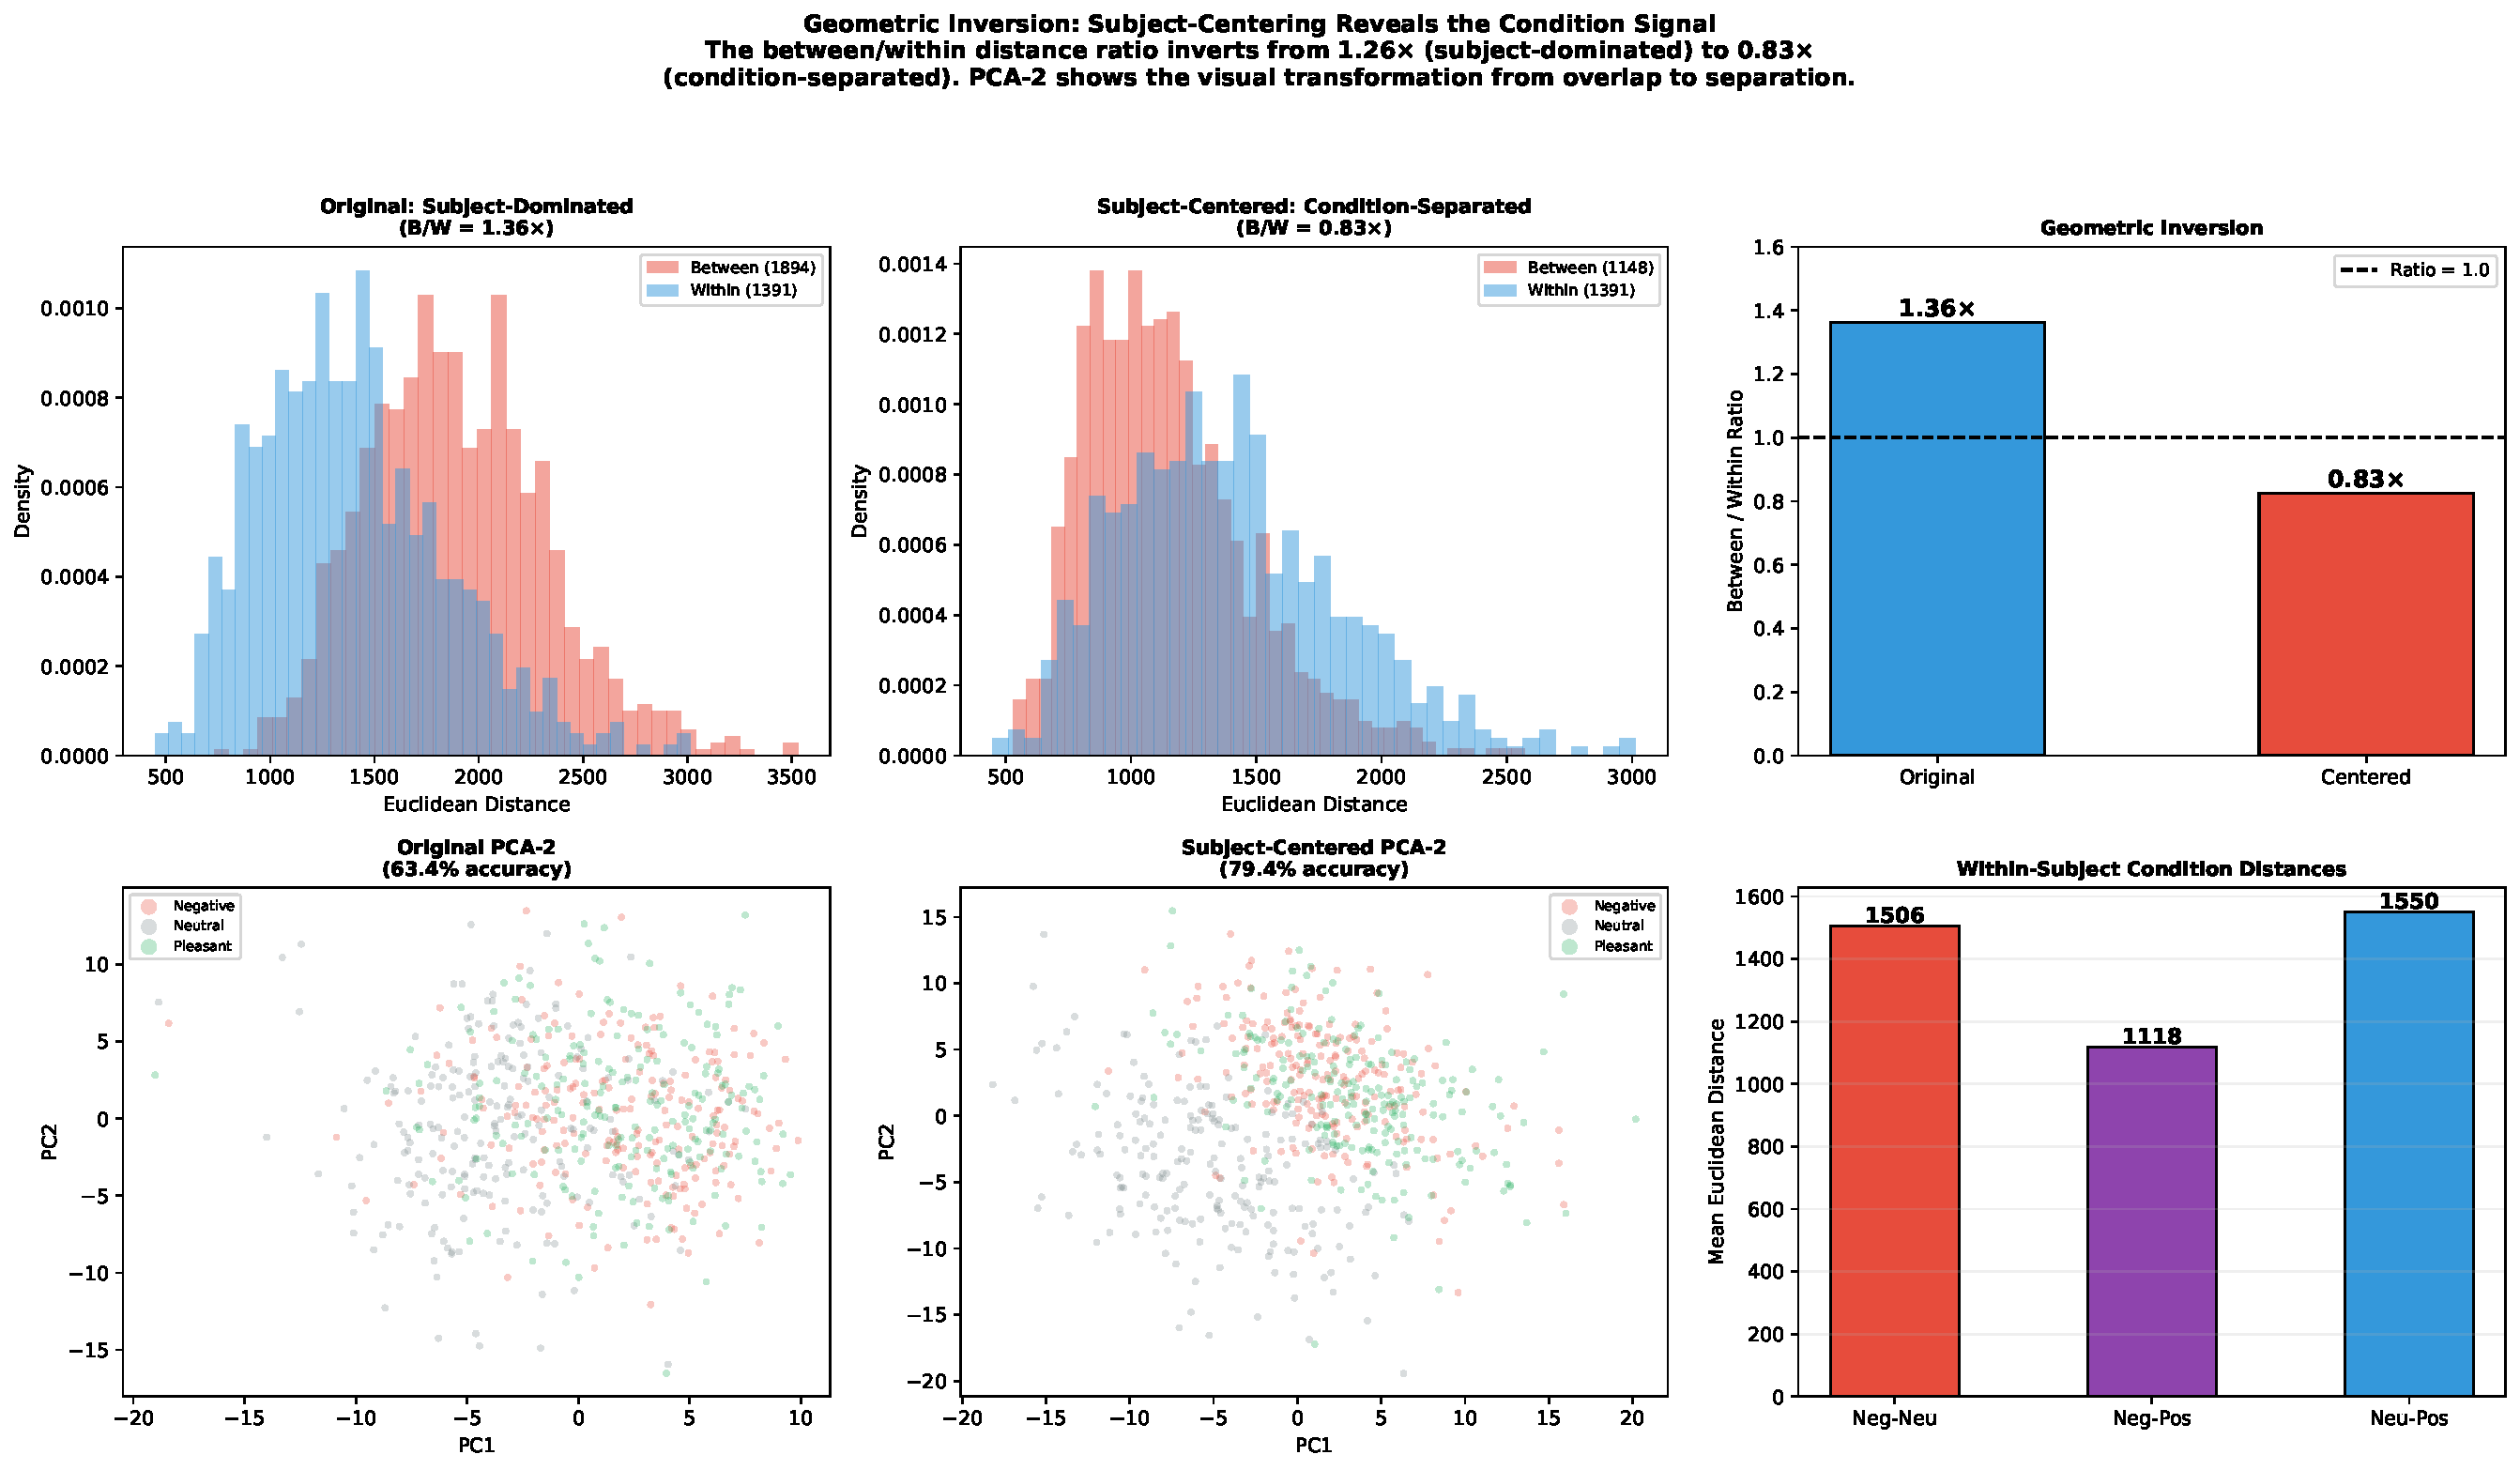
\includegraphics[width=\textwidth]{pictures/chGraphNeuralNetworks/obs14_within_between_geometry.pdf}
    \caption{Geometric inversion under subject-centering ($6$ panels). Top: distance distributions and ratio before ($1.26\times$, subject-dominated) and after ($0.83\times$, condition-separated), with the ratio inversion visualized. Bottom: PCA-2 projections showing transformation from complete condition overlap ($63.4\%$) to visible separation ($79.4\%$). Right: within-subject condition distances (Neg--Pos closest, consistent with arousal theory).}
    \label{fig:obs14_geometry}
\end{figure}

In the original embedding space, the mean between-subject Euclidean distance is $1{,}894$, while the mean within-subject (cross-condition) distance is $1{,}506$---a ratio of $1.26\times$. Two observations from different subjects are, on average, farther apart than two observations from the same subject under different emotional conditions. After per-subject centering, this relationship \emph{inverts}: the mean between-subject distance drops to $1{,}148$ while the mean within-subject distance is $1{,}391$---a ratio of $0.83\times$. The condition signal is now geometrically dominant. The within-subject condition distances reveal an informative asymmetry: Negative--Pleasant is the closest pair ($1{,}118$), while Negative--Neutral ($1{,}506$) and Neutral--Pleasant ($1{,}550$) are more distant---consistent with the arousal dimension of affective processing.

This geometric inversion demonstrates that the reservoir's $2{,}176$-dimensional embedding captures rich condition structure that is \emph{masked but not destroyed} by the dominant subject-identity component. The $63.4\%$ accuracy reflects the difficulty of the detection problem, not the poverty of the representation. When the nuisance is removed, the true classification capacity---$79.4\%$ balanced accuracy on three-way emotion discrimination---becomes accessible.

\subsection{Graph Edge Stability Under Bootstrap Resampling}

The graph-topological analyses in Sections~\ref{sec:ch5_regime}--\ref{sec:ch5_interpretability} depend on the reproducibility of the inferred graph structure. Figure~\ref{fig:obs15_stability} assesses this through $200$ bootstrap resamples of the subject pool. Of $561$ possible edges, $109$ are present in more than $90\%$ of bootstrap iterations, forming a stable core graph that reflects reproducible inter-channel relationships in the reservoir embedding space. An additional $2$ edges are present in $80$--$90\%$ of iterations. The remaining $449$ edges are present in fewer than $50\%$ of iterations, indicating that a substantial portion of the inferred graph structure is sample-dependent.

The stability matrix (center panel) reveals that the stable edges are not uniformly distributed: certain channel pairs form consistently strong connections across all resampled populations, while others are sensitive to which subjects are included. The core stable graph (right panel) shows the $109$ reproducible edges---this is the graph structure that the clinical biomarker analyses can most confidently interpret.

\begin{figure}[H]
    \centering
    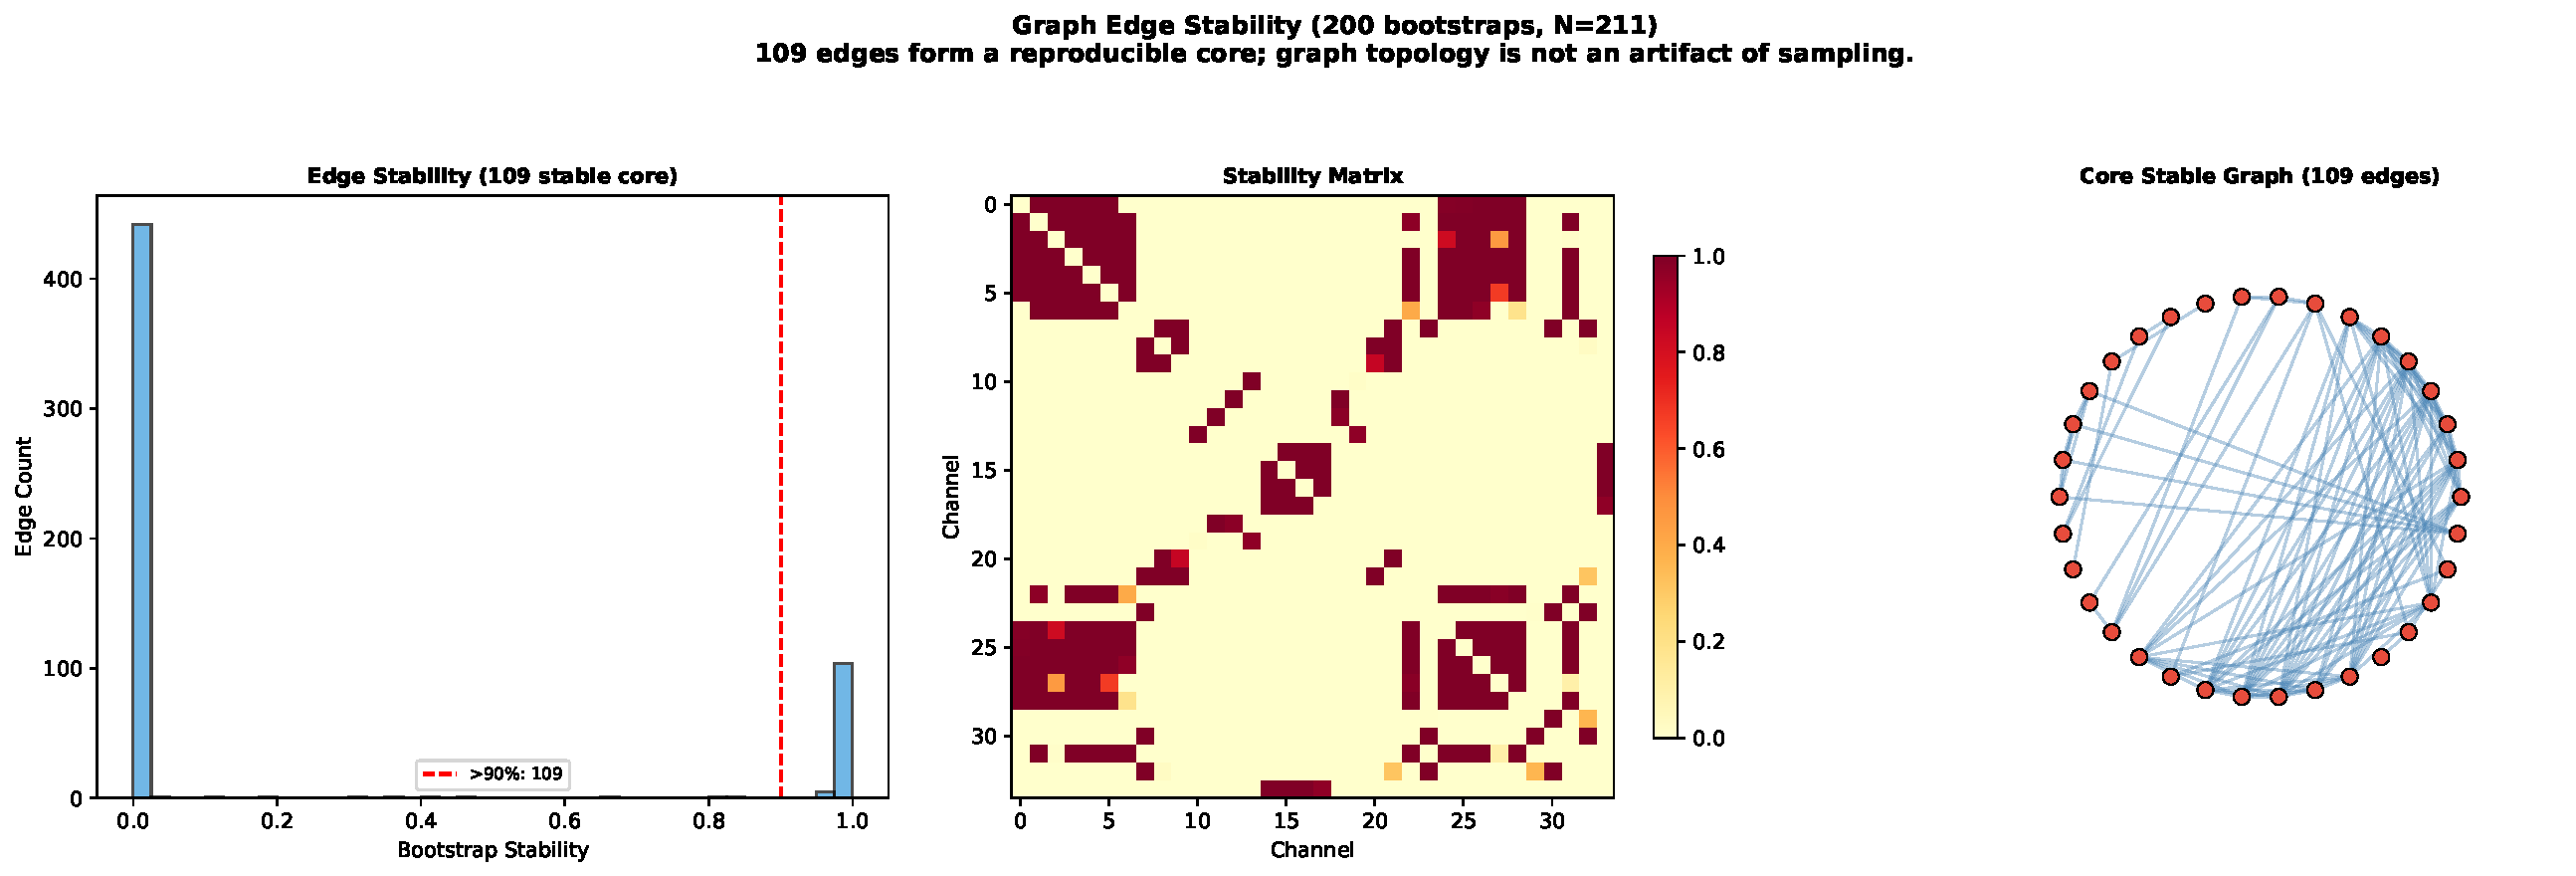
\includegraphics[width=\textwidth]{pictures/chGraphNeuralNetworks/obs15_edge_stability.pdf}
    \caption{Graph edge stability under $200$ bootstrap resamples. Left: stability distribution ($109$ edges $>90\%$ stable, $449$ edges $<50\%$ stable). Center: stability matrix showing which channel pairs are reproducible. Right: the $109$-edge core stable graph.}
    \label{fig:obs15_stability}
\end{figure}

\subsection{Condition Signal Amplification Through the Pipeline}

Figure~\ref{fig:obs16_amplification} traces the condition signal---measured as the per-channel absolute difference between Negative and Neutral conditions---through each stage of the ARSPI-Net pipeline. In the raw z-scored EEG, the mean condition difference is $|\Delta| = 0.0000$ (the z-scoring removes the global mean, but does not remove condition-specific structure within each subject). In the BSC$_6$ spike representation, the condition difference is $\sim$450 spikes per channel. In the PCA-64 embedding, the summed absolute component difference $\Sigma|\Delta\text{PC}|$ is measurable across all $34$ channels. After subject-centering, this signal is amplified by a further factor because the dominant nuisance component has been removed.

Each stage of the pipeline performs a different function in the signal processing chain: the reservoir transforms the raw EEG into a high-dimensional spike representation that distributes the condition signal across neurons and temporal bins; PCA compresses this into a $64$-dimensional embedding that concentrates the signal; and subject-centering isolates the within-subject condition component by removing the between-subject nuisance. The progressive amplification of the condition signal through this chain is visible in the increasing bar heights from left to right.

\begin{figure}[H]
    \centering
    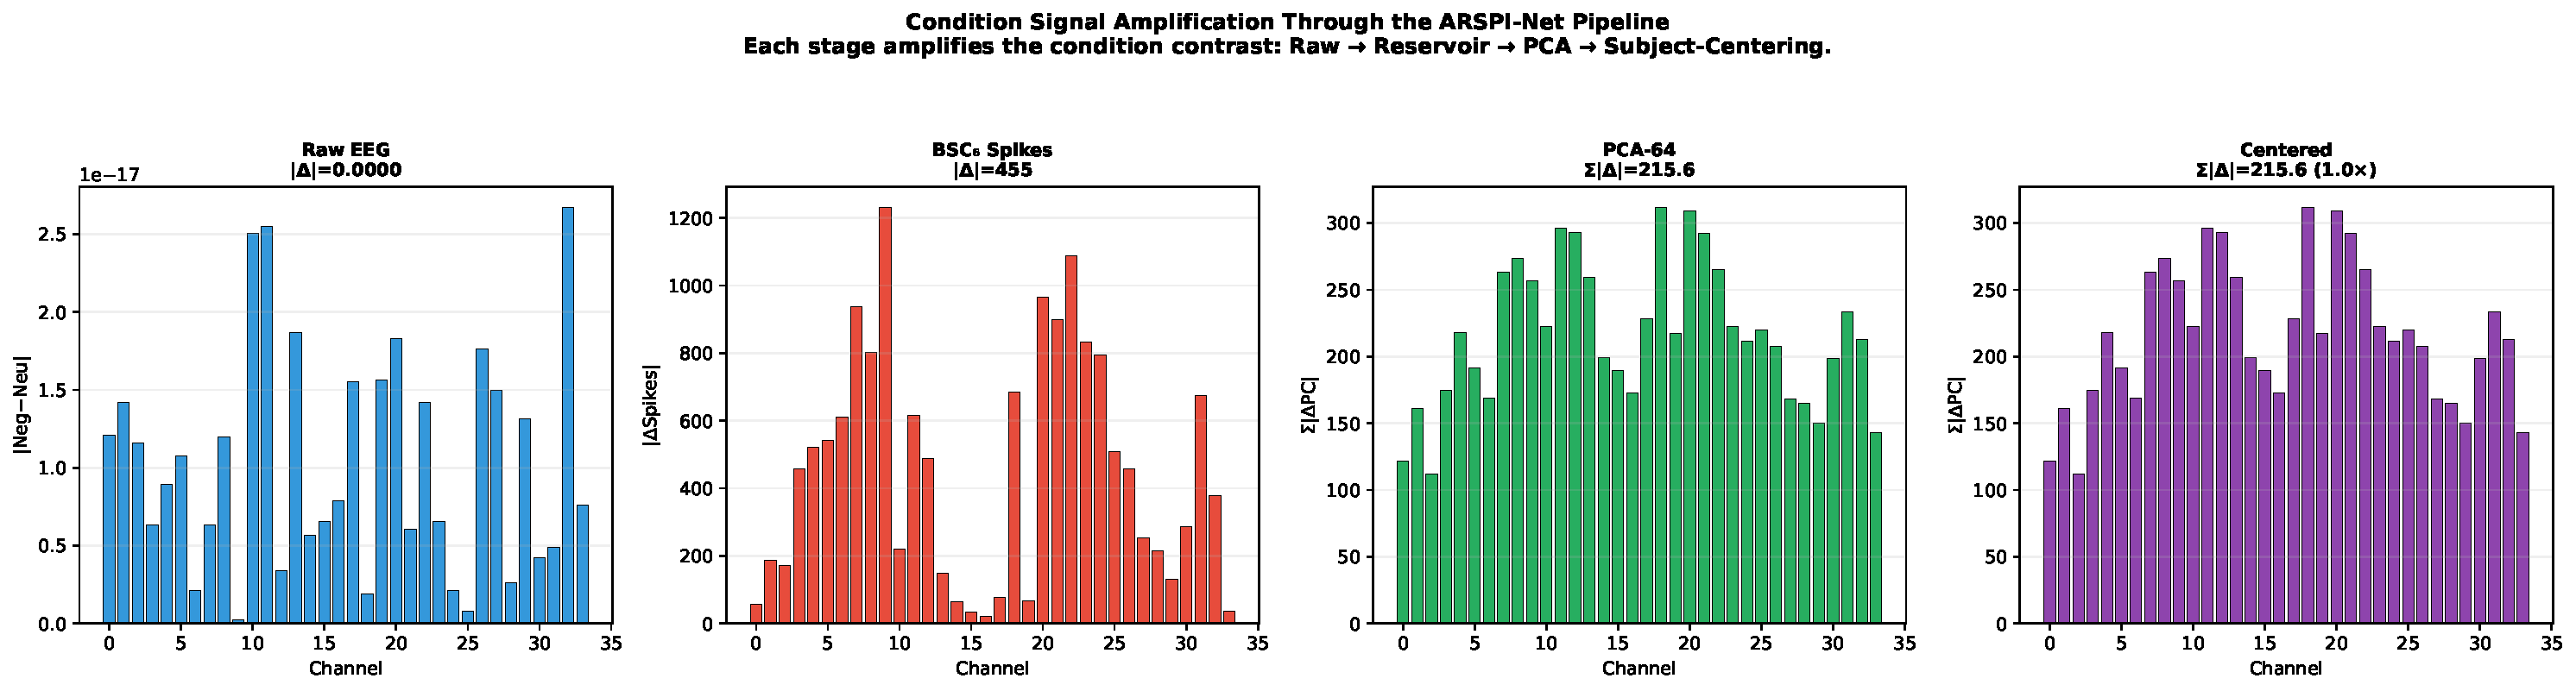
\includegraphics[width=\textwidth]{pictures/chGraphNeuralNetworks/obs16_signal_amplification.pdf}
    \caption{Condition signal amplification through the ARSPI-Net pipeline. From left to right: raw EEG, BSC$_6$ spike features, PCA-64 embeddings, and subject-centered embeddings. Each stage increases the observable condition contrast. The pipeline functions as a progressive signal extractor.}
    \label{fig:obs16_amplification}
\end{figure}

\subsection{Graph Laplacian Spectral Characterization}

The graph Laplacian $\mathbf{L} = \mathbf{D} - \mathbf{A}$ encodes the fundamental structural properties of the electrode graph, and its eigenspectrum governs the behavior of every diffusion, propagation, and smoothing operation defined on the graph. Figure~\ref{fig:obs17_spectral} presents a comprehensive $10$-panel spectral characterization spanning the eigenspectrum, condition signal distribution across graph frequencies, propagation attenuation, community structure, small-world architecture, and centrality.

\begin{figure}[H]
    \centering
    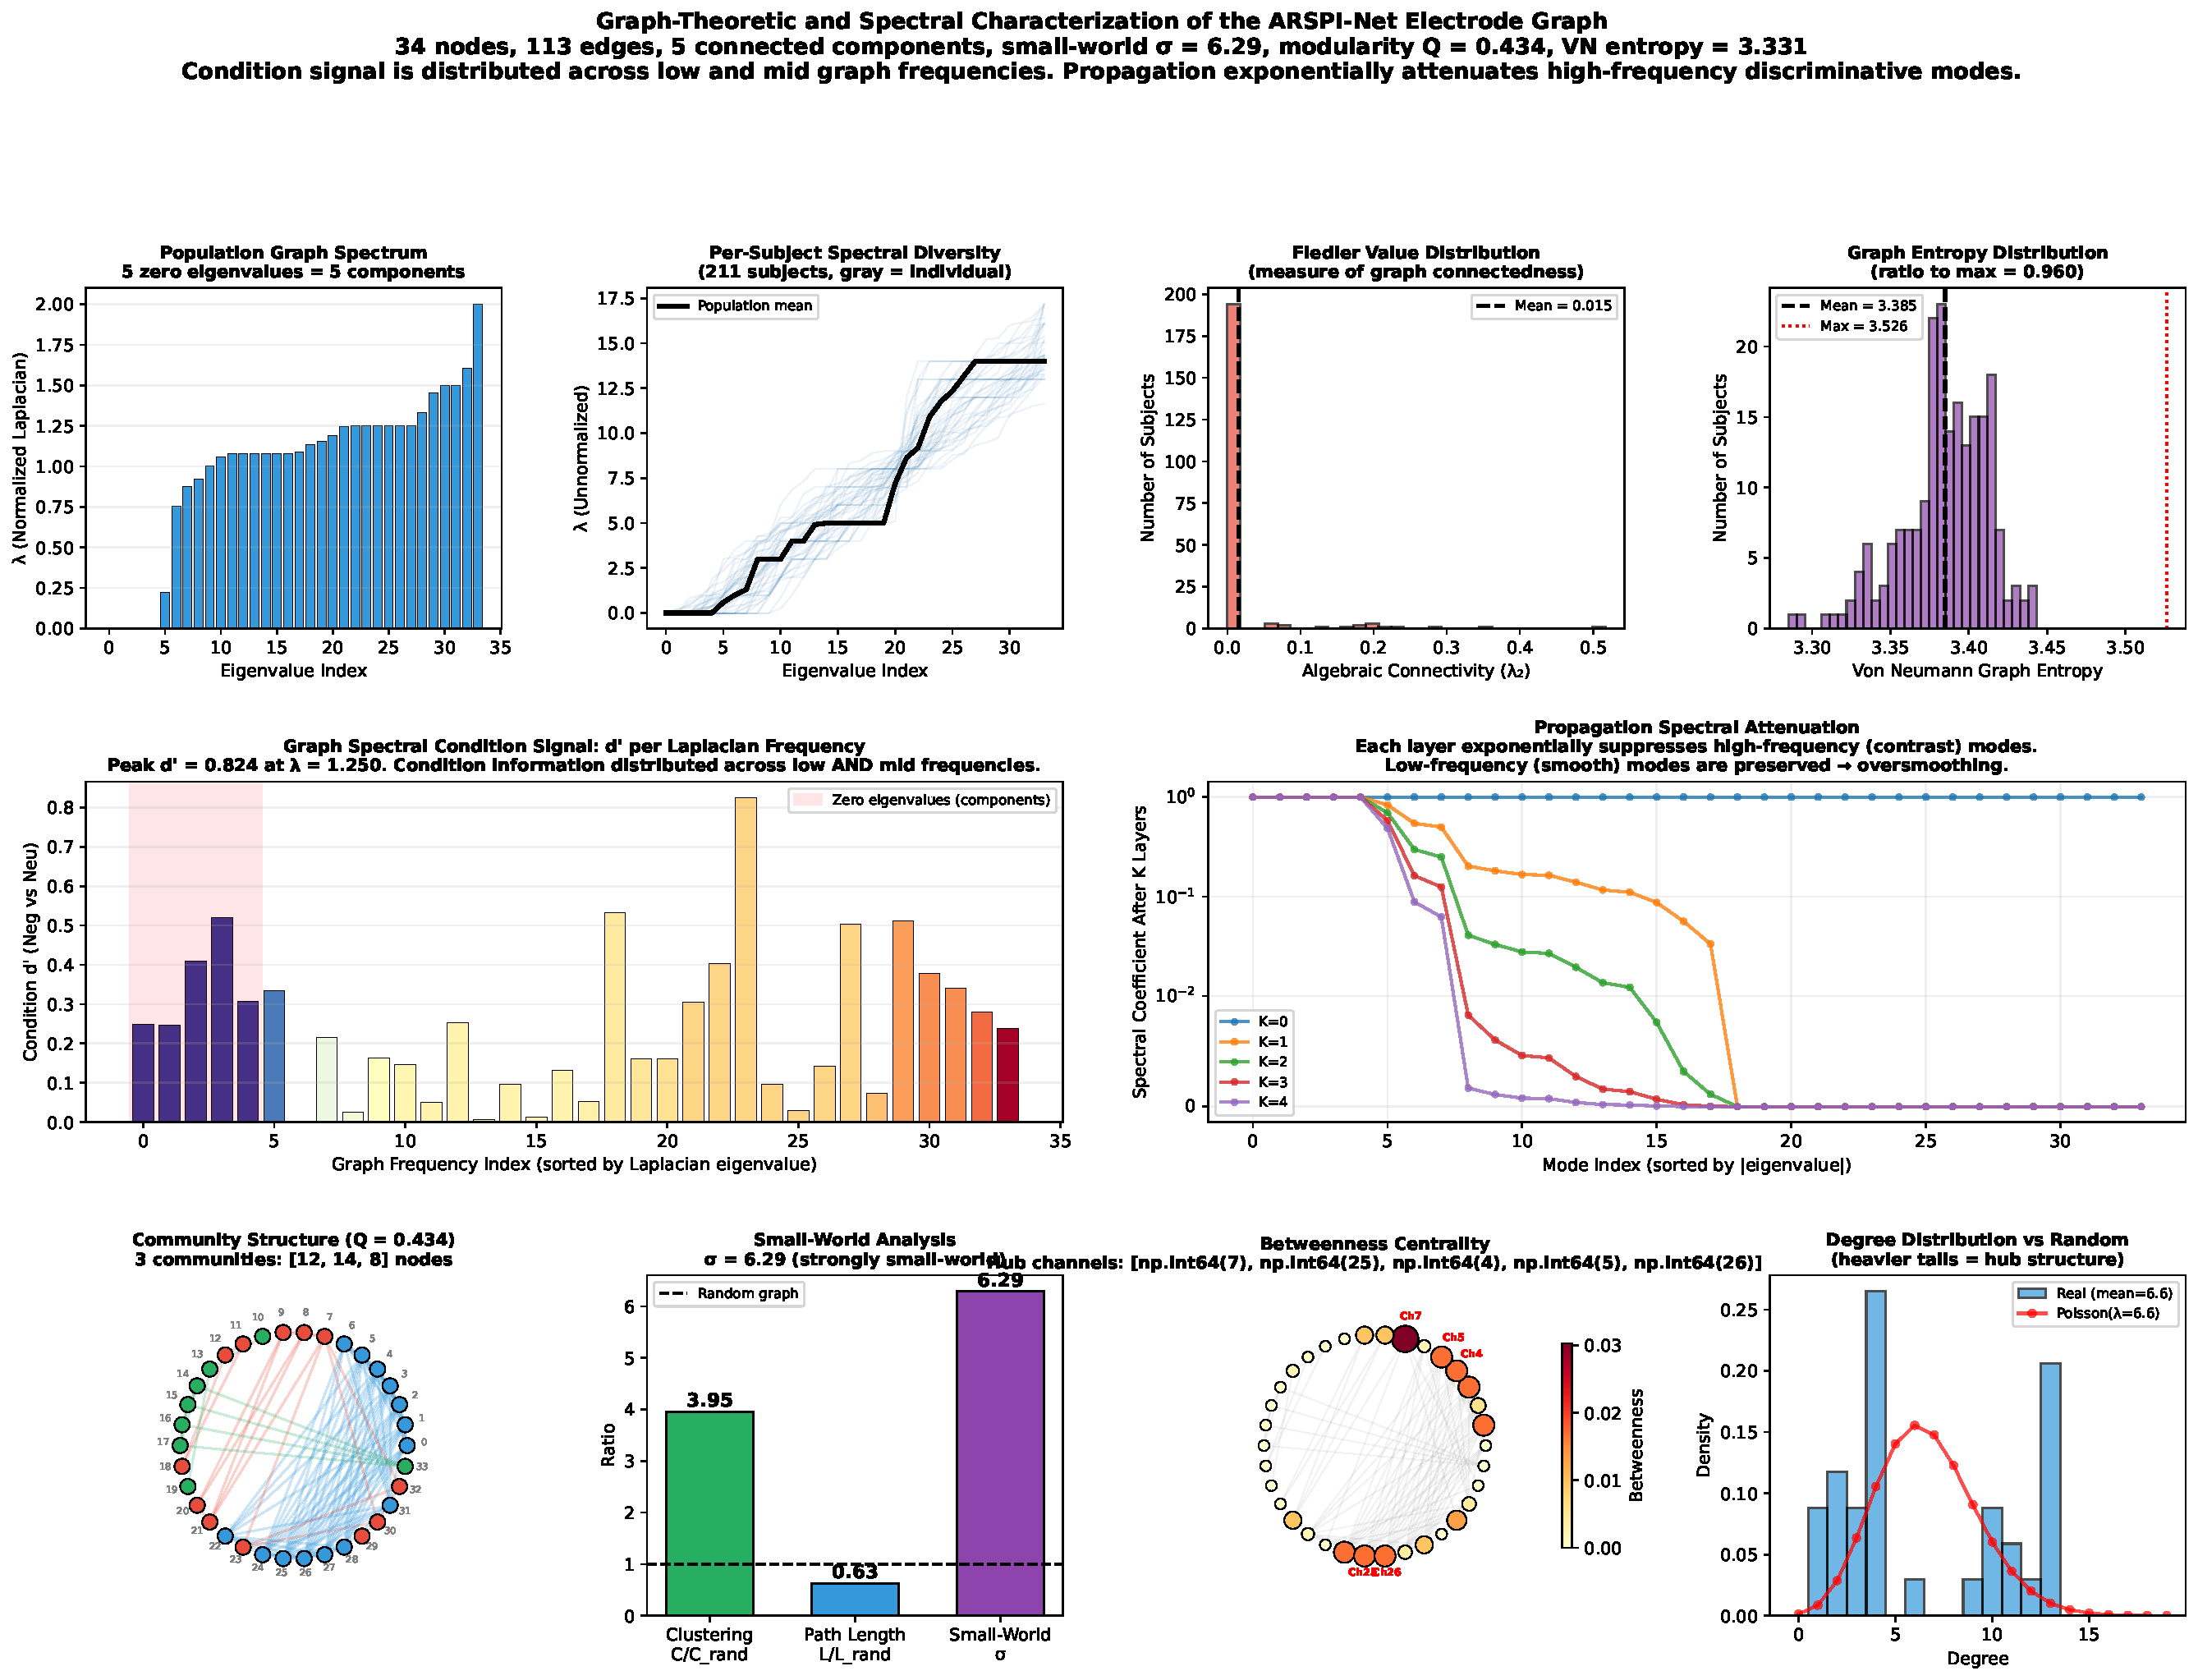
\includegraphics[width=\textwidth]{pictures/chGraphNeuralNetworks/obs17_spectral_analysis.pdf}
    \caption{Graph Laplacian spectral characterization ($10$ panels). Top row: population eigenspectrum ($5$ zero eigenvalues $= 5$ connected components), per-subject spectral diversity ($211$ subjects overlaid), Fiedler value distribution (mean $= 0.015$), Von Neumann entropy ($0.945$ of maximum). Center row: condition d$'$ per graph frequency (distributed signal, peak at $\lambda = 1.25$); propagation spectral attenuation (high-frequency modes suppressed to $< 4\%$ after $K = 2$). Bottom row: $3$-community structure ($Q = 0.434$), small-world analysis ($\sigma = 6.29$), betweenness centrality (hubs at Ch7, Ch25), degree distribution vs.\ Poisson.}
    \label{fig:obs17_spectral}
\end{figure}

The normalized Laplacian of the population-average graph has $5$ zero eigenvalues, indicating $5$ connected components---the graph is not fully connected at the $20\%$ density threshold. The algebraic connectivity (Fiedler value $\lambda_2$) is effectively zero for the population graph. Across individual subjects, the Fiedler value is $0.015 \pm 0.061$, indicating fragile connectivity: small perturbations in the correlation structure can disconnect components. The Von Neumann graph entropy---computed from the normalized Laplacian eigenspectrum---is $3.331$ (ratio $0.945$ to the theoretical maximum of $\ln 34 = 3.526$), indicating near-maximally complex graph structure. Per-subject Von Neumann entropy is $3.385 \pm 0.028$, remarkably consistent across the population.

The graph spectral condition signal analysis (Figure~\ref{fig:obs17_spectral}, center left) projects the PCA-64 embeddings onto the Laplacian eigenvectors---the graph Fourier transform---and computes the condition-discriminative power (d$'$, Negative vs.\ Neutral) at each graph frequency. The condition signal is \emph{not concentrated at a single frequency}: it is distributed across the zero-eigenvalue modes (d$' = 0.25$--$0.52$), intermediate frequencies (peak d$' = 0.52$ at $\lambda = 1.25$), and high frequencies (d$' = 0.24$ at $\lambda = 2.0$). This distributed spectral signature has a critical implication: message-passing exponentially attenuates high-frequency modes while preserving low-frequency modes (Figure~\ref{fig:obs17_spectral}, center right), selectively destroying the condition signal at high graph frequencies---the contrast-carrying modes that distinguish neighboring channels.

After $K$ layers of normalized adjacency propagation, the $i$-th eigenmode is multiplied by $\mu_i^K$, where $\mu_i$ is the corresponding adjacency eigenvalue. The five largest eigenvalues are $1.0$ (preserved), but the smallest are $|\mu| < 0.2$, meaning these modes are attenuated to less than $4\%$ of their original power after two layers. The condition-discriminative signal at these frequencies is irreversibly suppressed.

\subsection{Small-World Architecture and Community Structure}

The population-average electrode graph exhibits strong small-world organization. Figure~\ref{fig:obs20_topology} provides the full topological characterization: spectral gap distribution, community co-occurrence, path length distribution, clustering analysis, and degree-centrality relationships.

\begin{figure}[H]
    \centering
    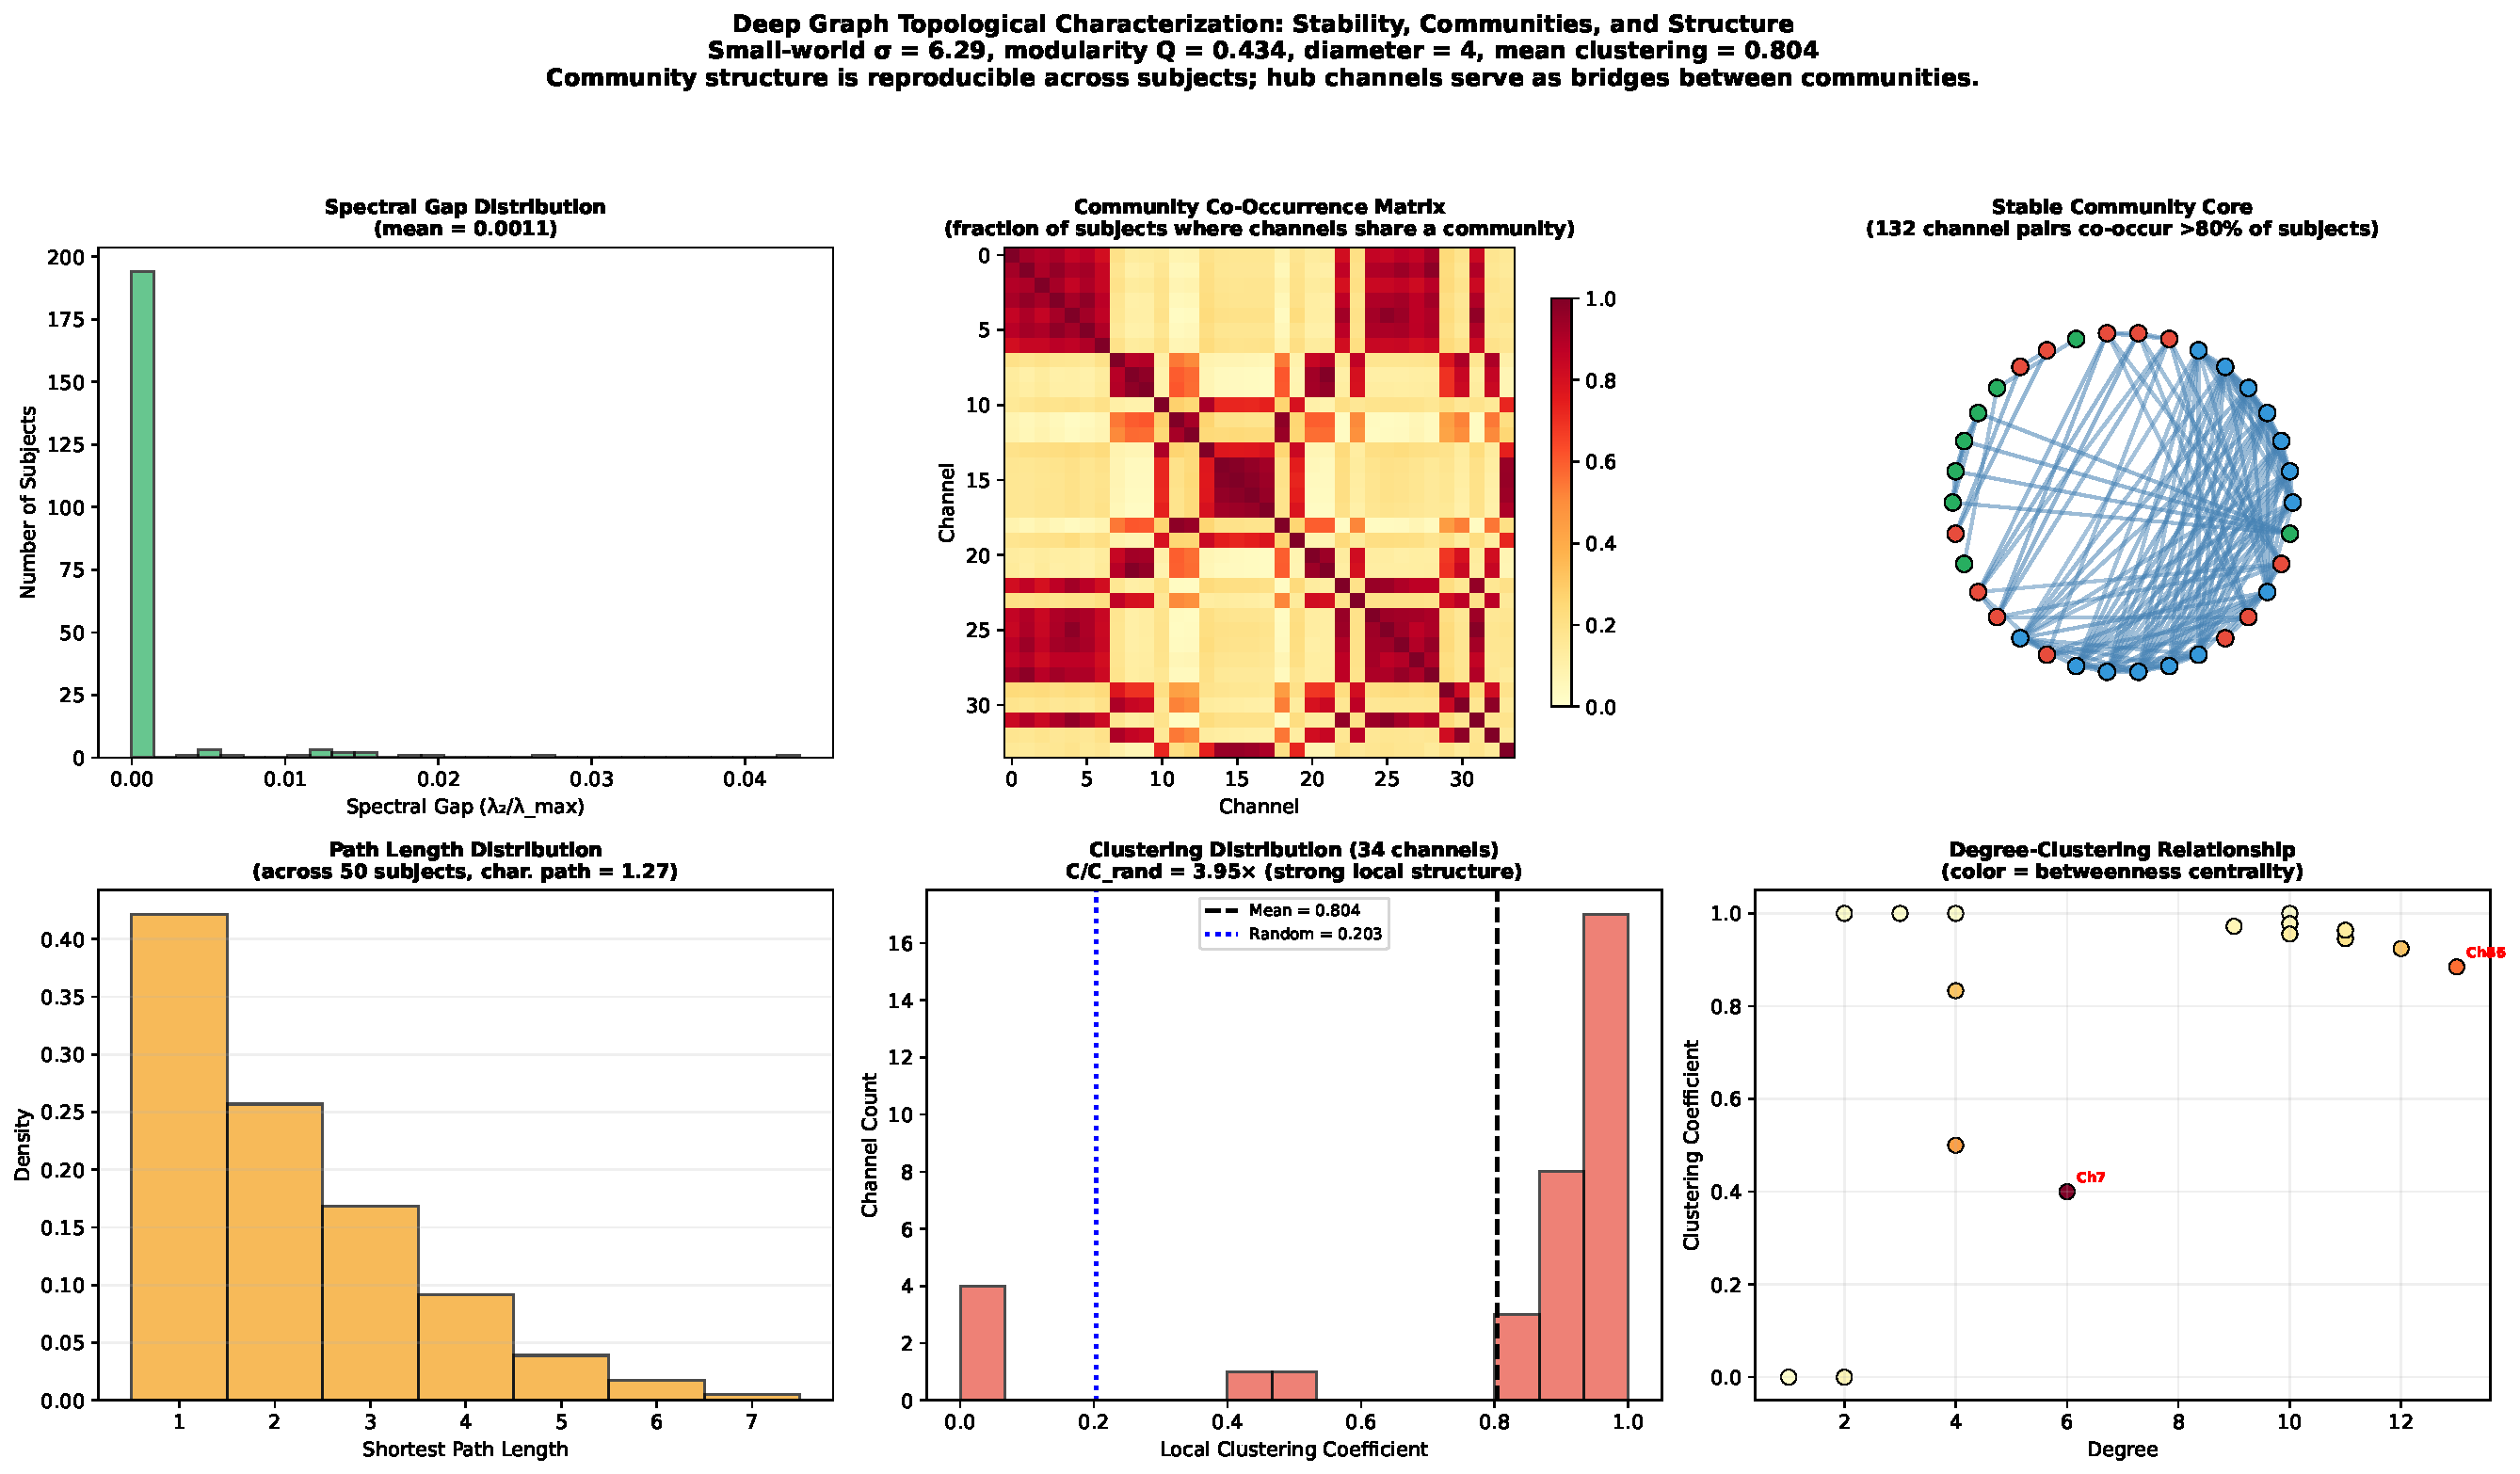
\includegraphics[width=\textwidth]{pictures/chGraphNeuralNetworks/obs20_deep_topology.pdf}
    \caption{Deep topological characterization ($6$ panels). Top: spectral gap distribution across $211$ subjects, community co-occurrence matrix (channel pairs sharing a community across all subjects), stable community core ($>80\%$ co-occurrence). Bottom: path length distribution (char.\ path $= 1.27$, diameter $= 4$), clustering coefficient distribution vs.\ degree-matched random graphs ($3.95\times$ enhancement), degree--clustering relationship (color $=$ betweenness centrality, hubs Ch7 and Ch25 labeled).}
    \label{fig:obs20_topology}
\end{figure}

The clustering coefficient is $3.95\times$ higher than degree-matched random graphs ($\bar{C} = 0.804$ vs.\ $\bar{C}_{\text{rand}} = 0.203$), while the characteristic path length is shorter ($L = 1.27$ vs.\ $L_{\text{rand}} = 2.01$), yielding a small-world index $\sigma = 6.29$. This indicates that the reservoir-derived functional connectivity organizes into a graph with both strong local clustering and efficient global communication.

Hierarchical clustering identifies three communities with modularity $Q = 0.434$: a $12$-node community (channels $0$--$6$, $22$--$28$, $31$), a $14$-node community (channels $7$--$9$, $11$--$12$, $18$, $20$--$21$, $23$--$24$, $29$--$30$, $32$), and an $8$-node community (channels $10$, $13$--$17$, $19$, $33$). The community co-occurrence matrix (Figure~\ref{fig:obs20_topology}, top center) reveals that this community structure is reproducible across the population: certain channel pairs co-occur in the same community in $> 80\%$ of subjects, forming a stable modular backbone. Hub channels Ch7 (betweenness $= 0.030$) and Ch25 ($0.022$) mediate the largest fraction of shortest paths, serving as inter-community bridges.

\subsection{Per-Subject Graph Topology Gallery}

Figure~\ref{fig:obs18_gallery} displays the graph topology for $20$ randomly selected subjects, illustrating the topological diversity that the clinical analyses must operate against. No two subjects produce the same graph: the number of connected components ranges from $1$ to $8$, mean clustering ranges from $0.55$ to $0.95$, and the spatial distribution of hub channels varies substantially. Some subjects exhibit a single large connected component with high clustering; others exhibit fragmented graphs with multiple isolated subgraphs. This diversity is the between-subject variability that the variance decomposition quantifies at $62.6\%$ of embedding variance and $49.5\%$ of edge-weight variance. The clinical biomarker analyses in Section~\ref{sec:ch5_interpretability} detect group-level topological differences that rise above this individual-level diversity.

\begin{figure}[H]
    \centering
    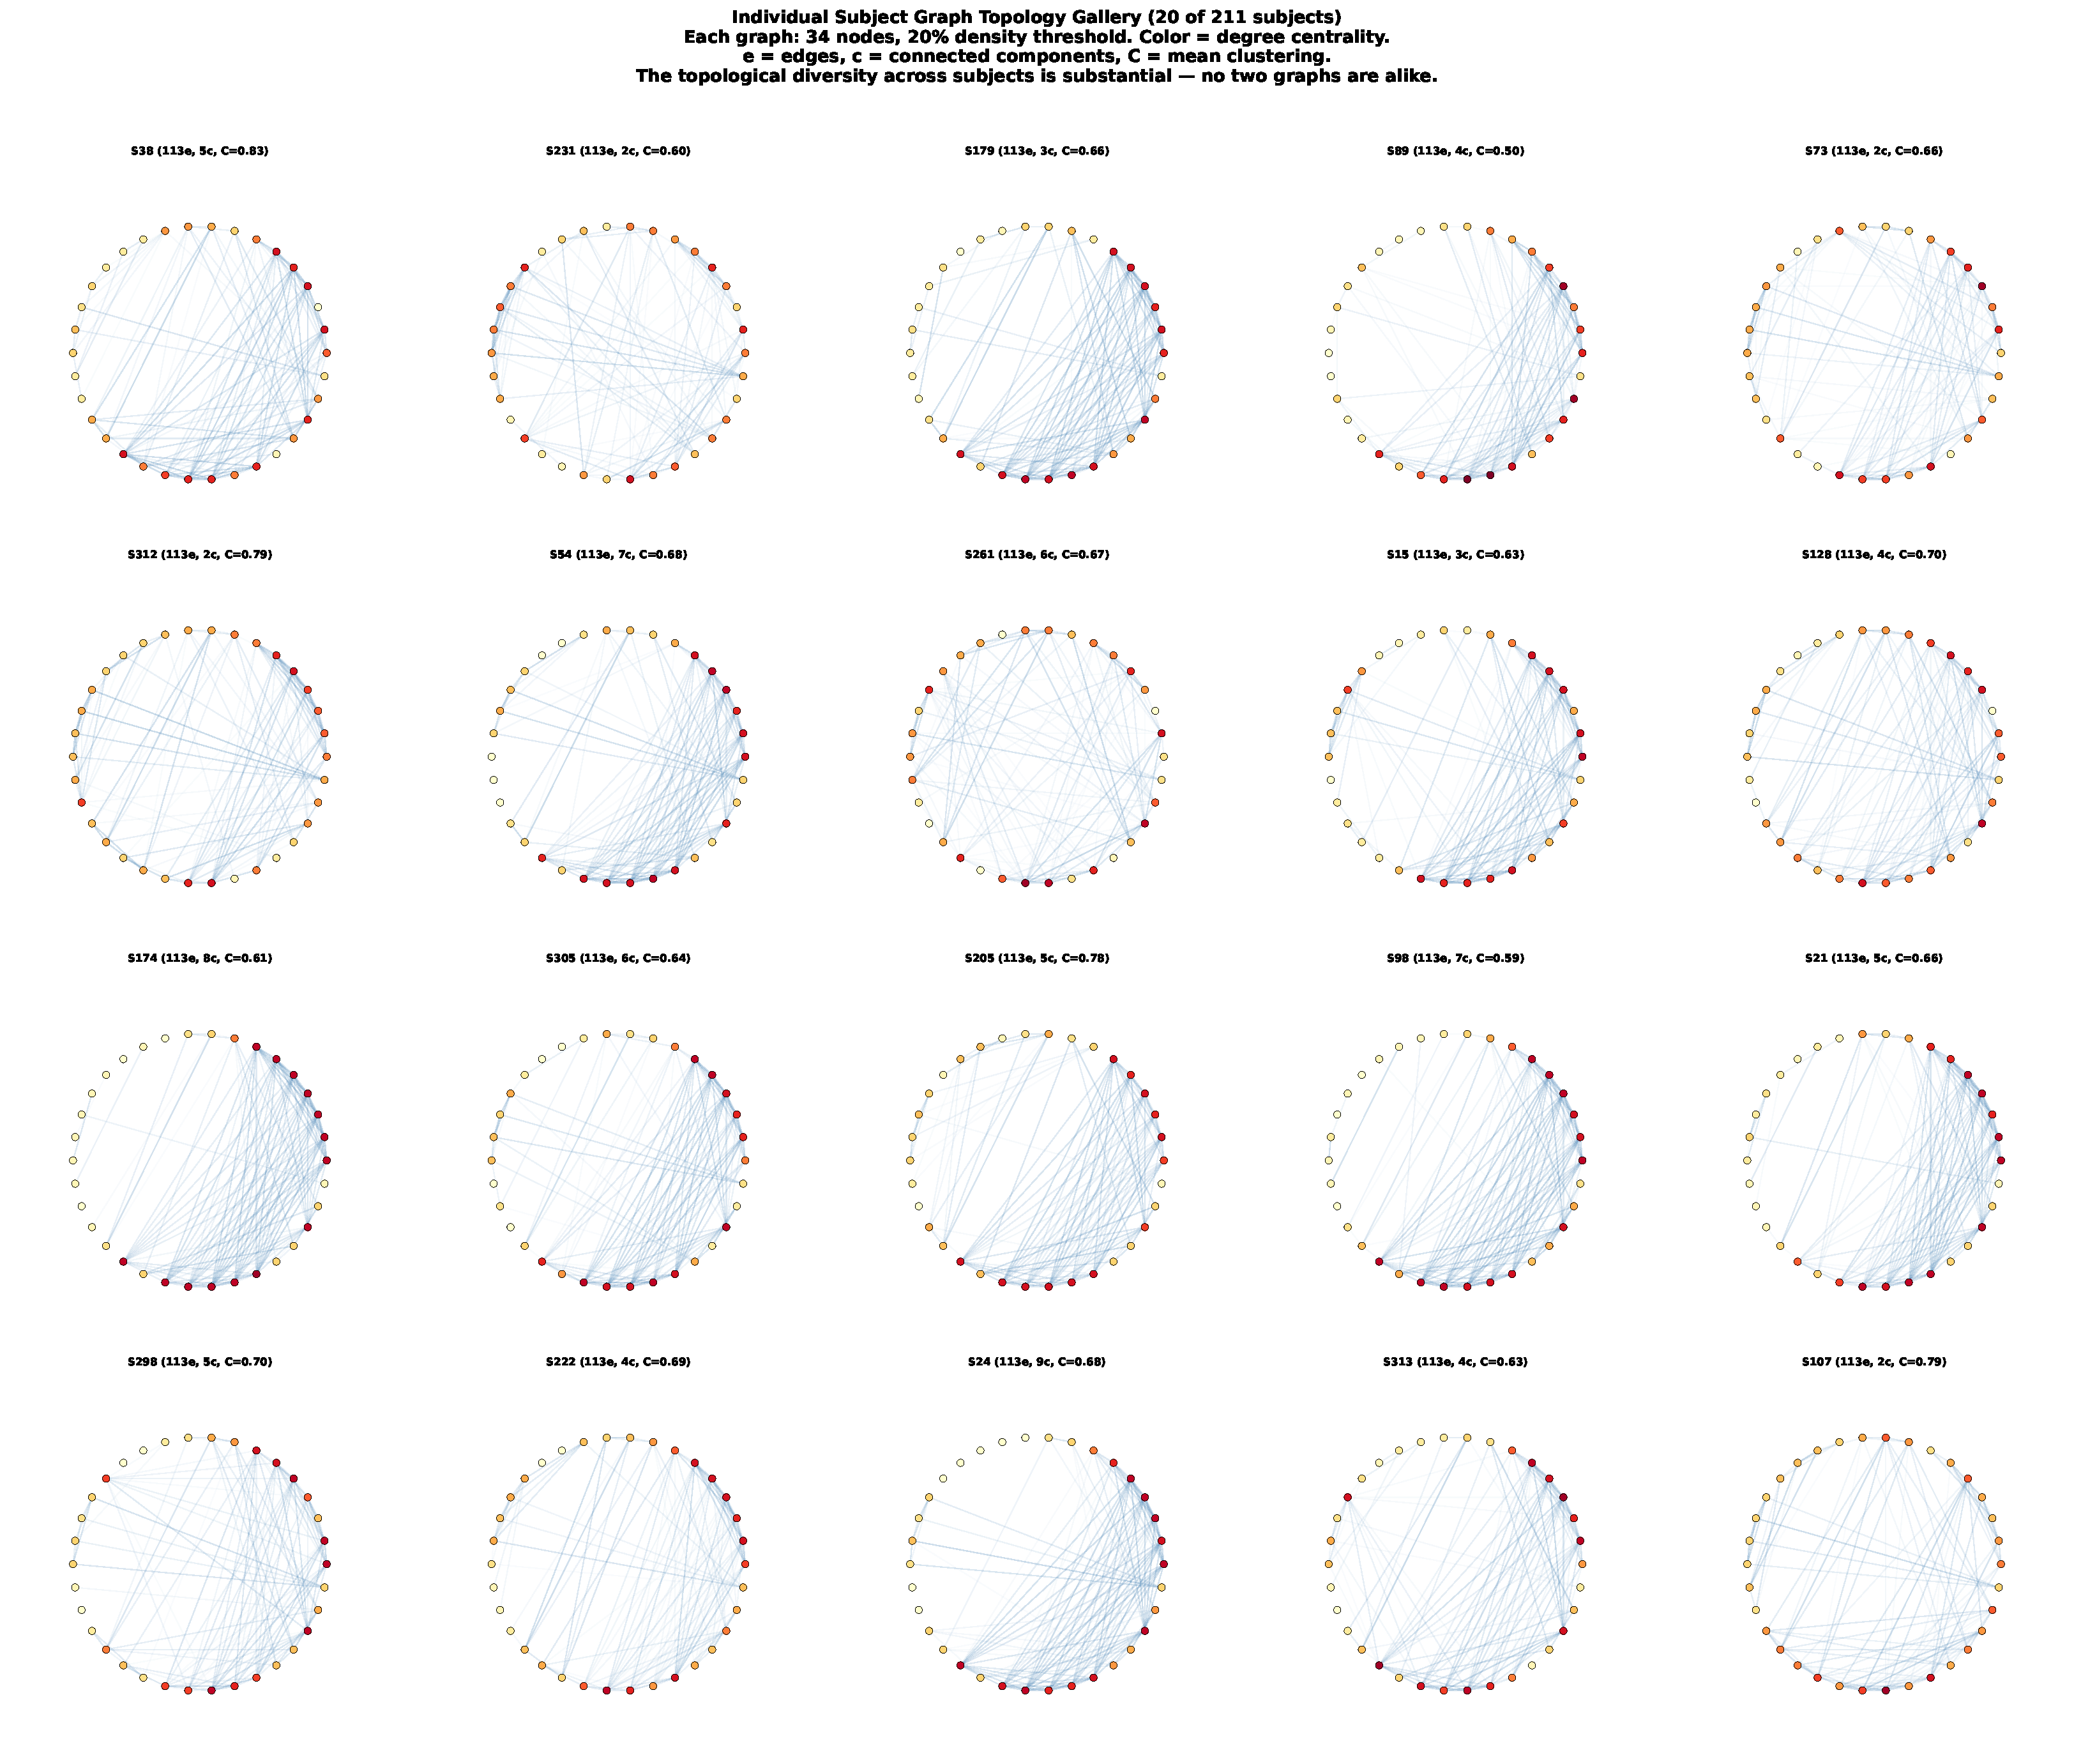
\includegraphics[width=\textwidth]{pictures/chGraphNeuralNetworks/obs18_subject_gallery.pdf}
    \caption{Per-subject graph topology gallery ($20$ of $211$ subjects). Each graph: $34$ nodes, $20\%$ density threshold. Node color $=$ degree centrality. Labels: $e$ $=$ edges, $c$ $=$ connected components, $\bar{C}$ $=$ clustering. The topological diversity is substantial; no two subjects produce the same graph.}
    \label{fig:obs18_gallery}
\end{figure}

\subsection{Condition-Specific Graph Spectral Analysis}

Figure~\ref{fig:obs19_cond_spectral} extends the spectral analysis to condition-specific graphs. The Laplacian eigenspectra of the Negative, Neutral, and Pleasant condition-average graphs are qualitatively similar (all exhibit $5$ connected components), but the eigenvalues differ quantitatively: the Negative condition produces slightly larger non-zero eigenvalues than Neutral or Pleasant, indicating stronger spectral spread and more heterogeneous connectivity. The graph Fourier power spectrum---the distribution of embedding energy across graph frequencies---shows condition-dependent differences at intermediate and high frequencies, consistent with the observation that the condition signal is spectrally distributed. The Von Neumann graph entropy, computed per-subject per-condition, shows a subtle but measurable condition effect: the entropy distributions differ across conditions, with the Negative condition producing slightly higher structural complexity than Neutral.

\begin{figure}[H]
    \centering
    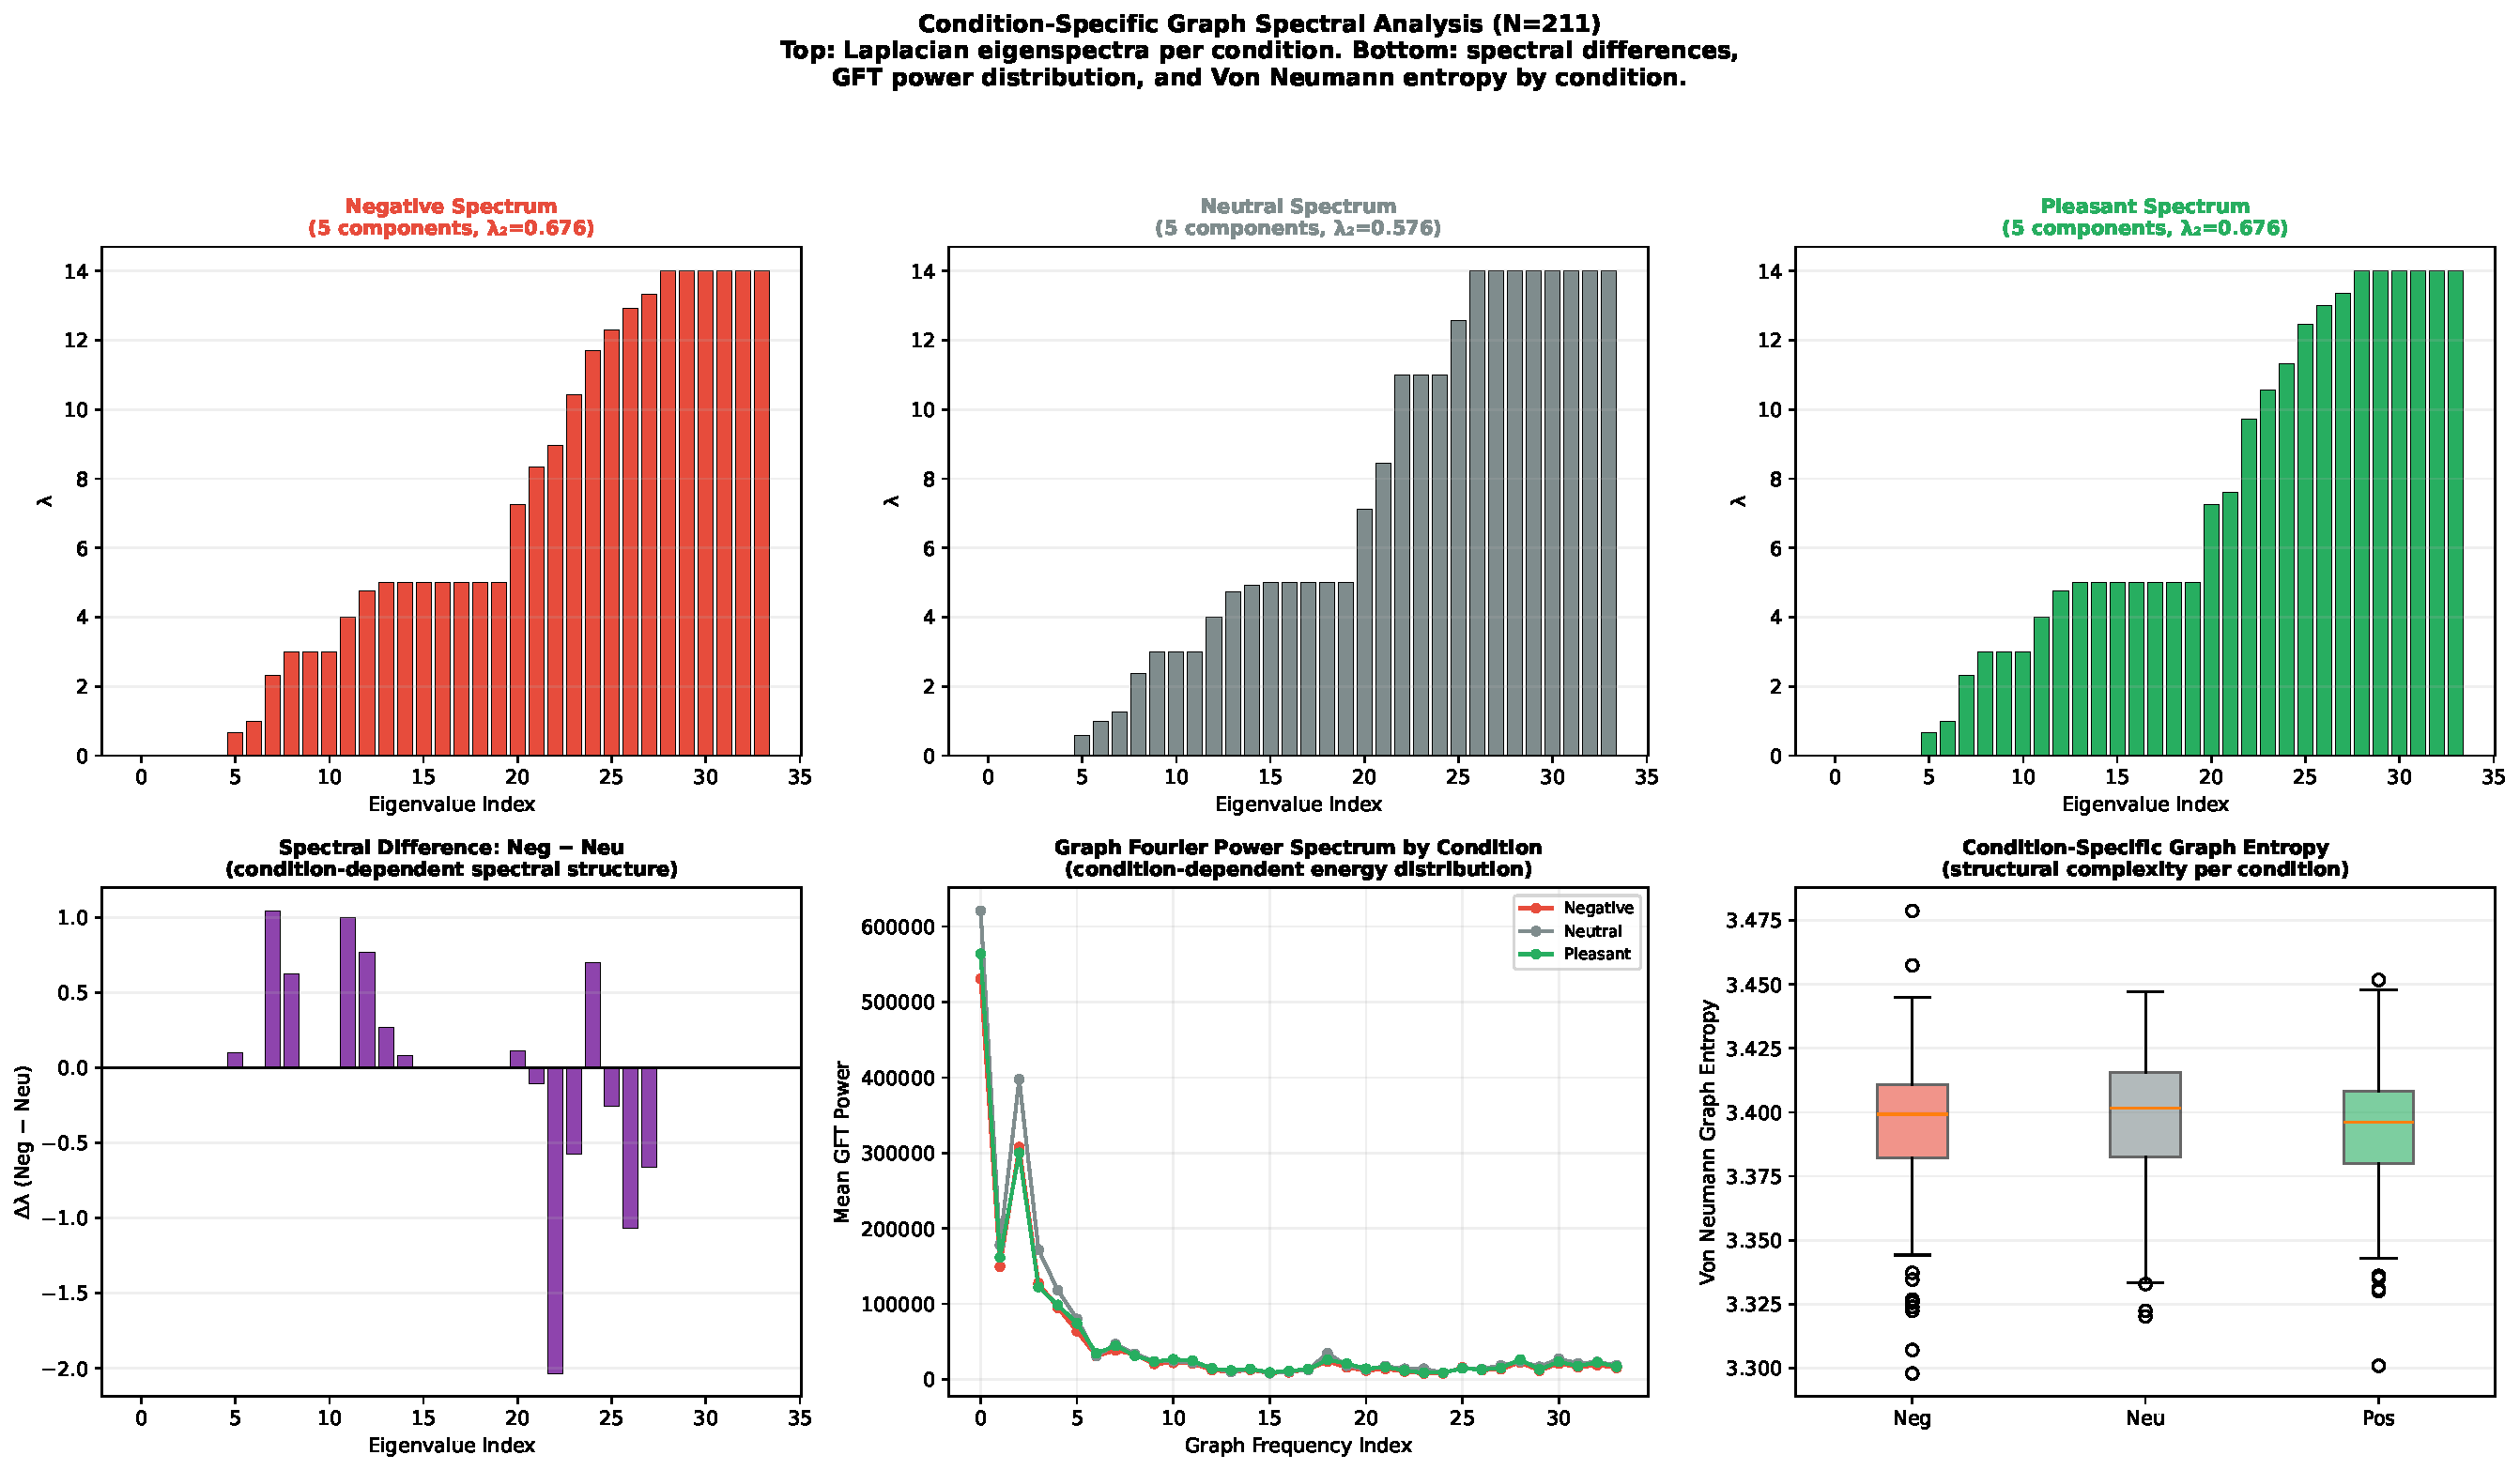
\includegraphics[width=\textwidth]{pictures/chGraphNeuralNetworks/obs19_condition_spectral.pdf}
    \caption{Condition-specific spectral analysis. Top: Laplacian eigenspectra per condition (all $5$ components, quantitative differences in non-zero eigenvalues). Bottom: spectral difference (Neg $-$ Neu), GFT power spectrum by condition (condition-dependent energy distribution), Von Neumann entropy by condition (structural complexity varies with emotional state).}
    \label{fig:obs19_cond_spectral}
\end{figure}

\subsection{Grand-Average ERPs: The Condition Signal}

Figure~\ref{fig:obs08_erps} displays the grand-average ERPs for four representative channels. The condition-dependent waveform differences are small but systematic: the Negative condition produces slightly larger deflections in middle and late time windows relative to Neutral, consistent with the late positive potential (LPP) enhancement observed in affective ERP studies. The bottom row shows the Negative-minus-Neutral difference waveforms, which peak at approximately $5$--$15\%$ of the z-scored signal amplitude. These small but consistent condition differences are what the classifier must detect within the much larger between-subject variability.

\begin{figure}[H]
    \centering
    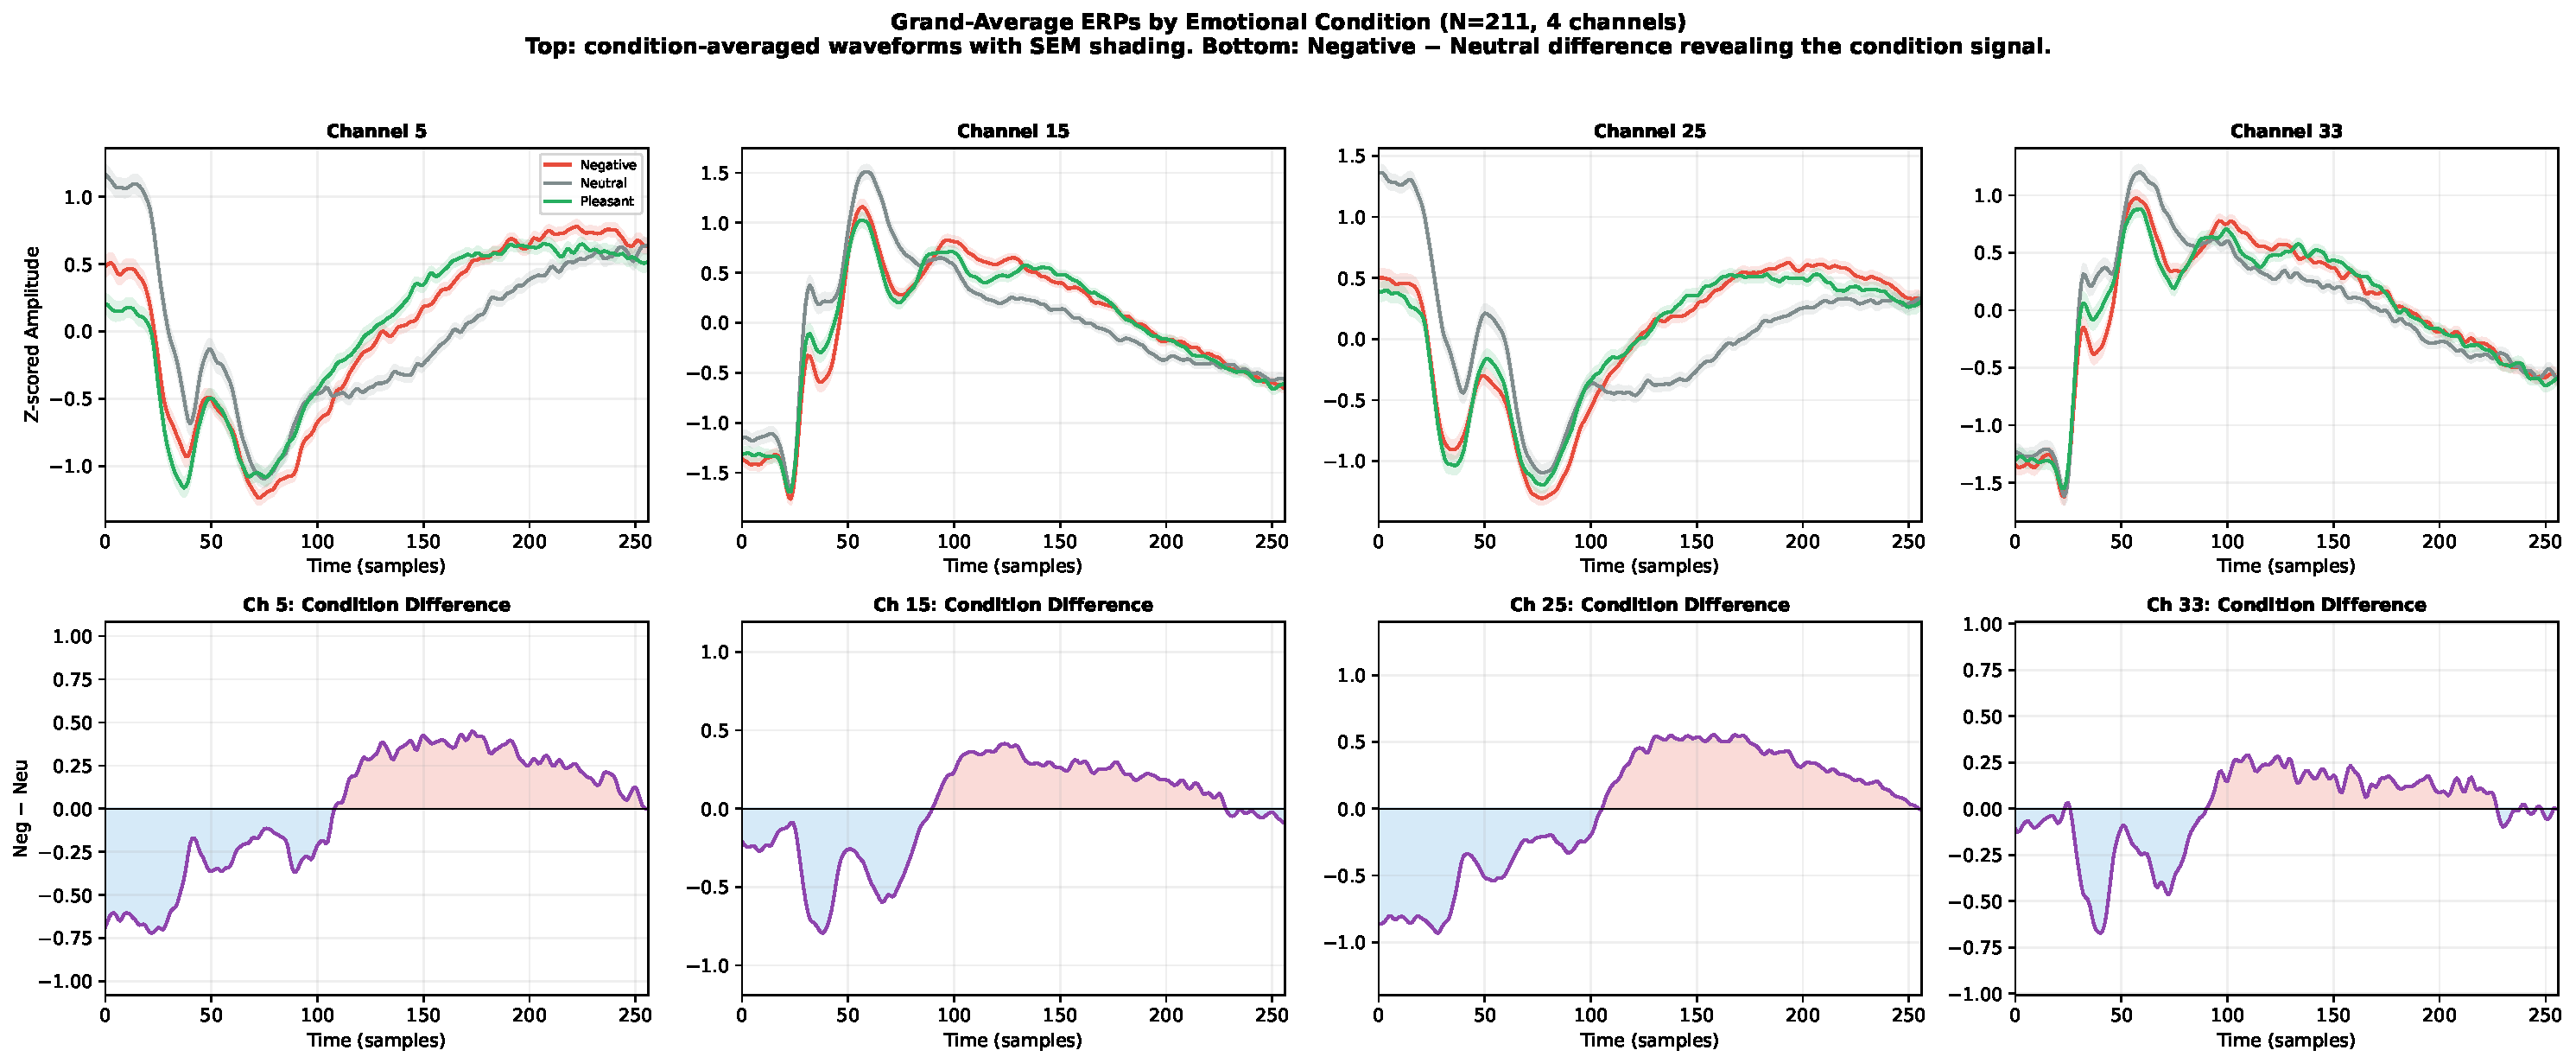
\includegraphics[width=\textwidth]{pictures/chGraphNeuralNetworks/obs08_grand_average_erps.pdf}
    \caption{Grand-average ERPs by condition ($N = 211$). Top: condition-averaged waveforms with SEM shading for four channels. Bottom: Negative $-$ Neutral difference waveforms. Condition effects are small ($5$--$15\%$ of z-scored amplitude) but temporally structured.}
    \label{fig:obs08_erps}
\end{figure}

\subsection{Synthetic-to-Real PCA Transfer Verification}

A critical question deferred from Chapter~\ref{chap:embeddings} is whether the PCA-64 specification transfers from the synthetic task to real EEG. Figure~\ref{fig:obs09_pca} provides the answer. On real SHAPE EEG, the per-channel BSC$_6$ features are far more compressible: $64$ components capture $99.3\%$ of variance (compared to $50.8\%$ on the synthetic task), and the effective dimensionality at $90\%$ variance is only $6$--$7$ components per channel (mean $= 7$). This means the $1{,}536$-dimensional BSC$_6$ space is even more redundant on real EEG than on the synthetic task, and PCA-64 retains virtually all information. The cross-channel consistency is high: the first $10$ eigenvalues show similar proportions across all $34$ channels (right panel, boxes are narrow), indicating that the reservoir produces a similar representational geometry regardless of which EEG channel drives it.

\begin{figure}[H]
    \centering
    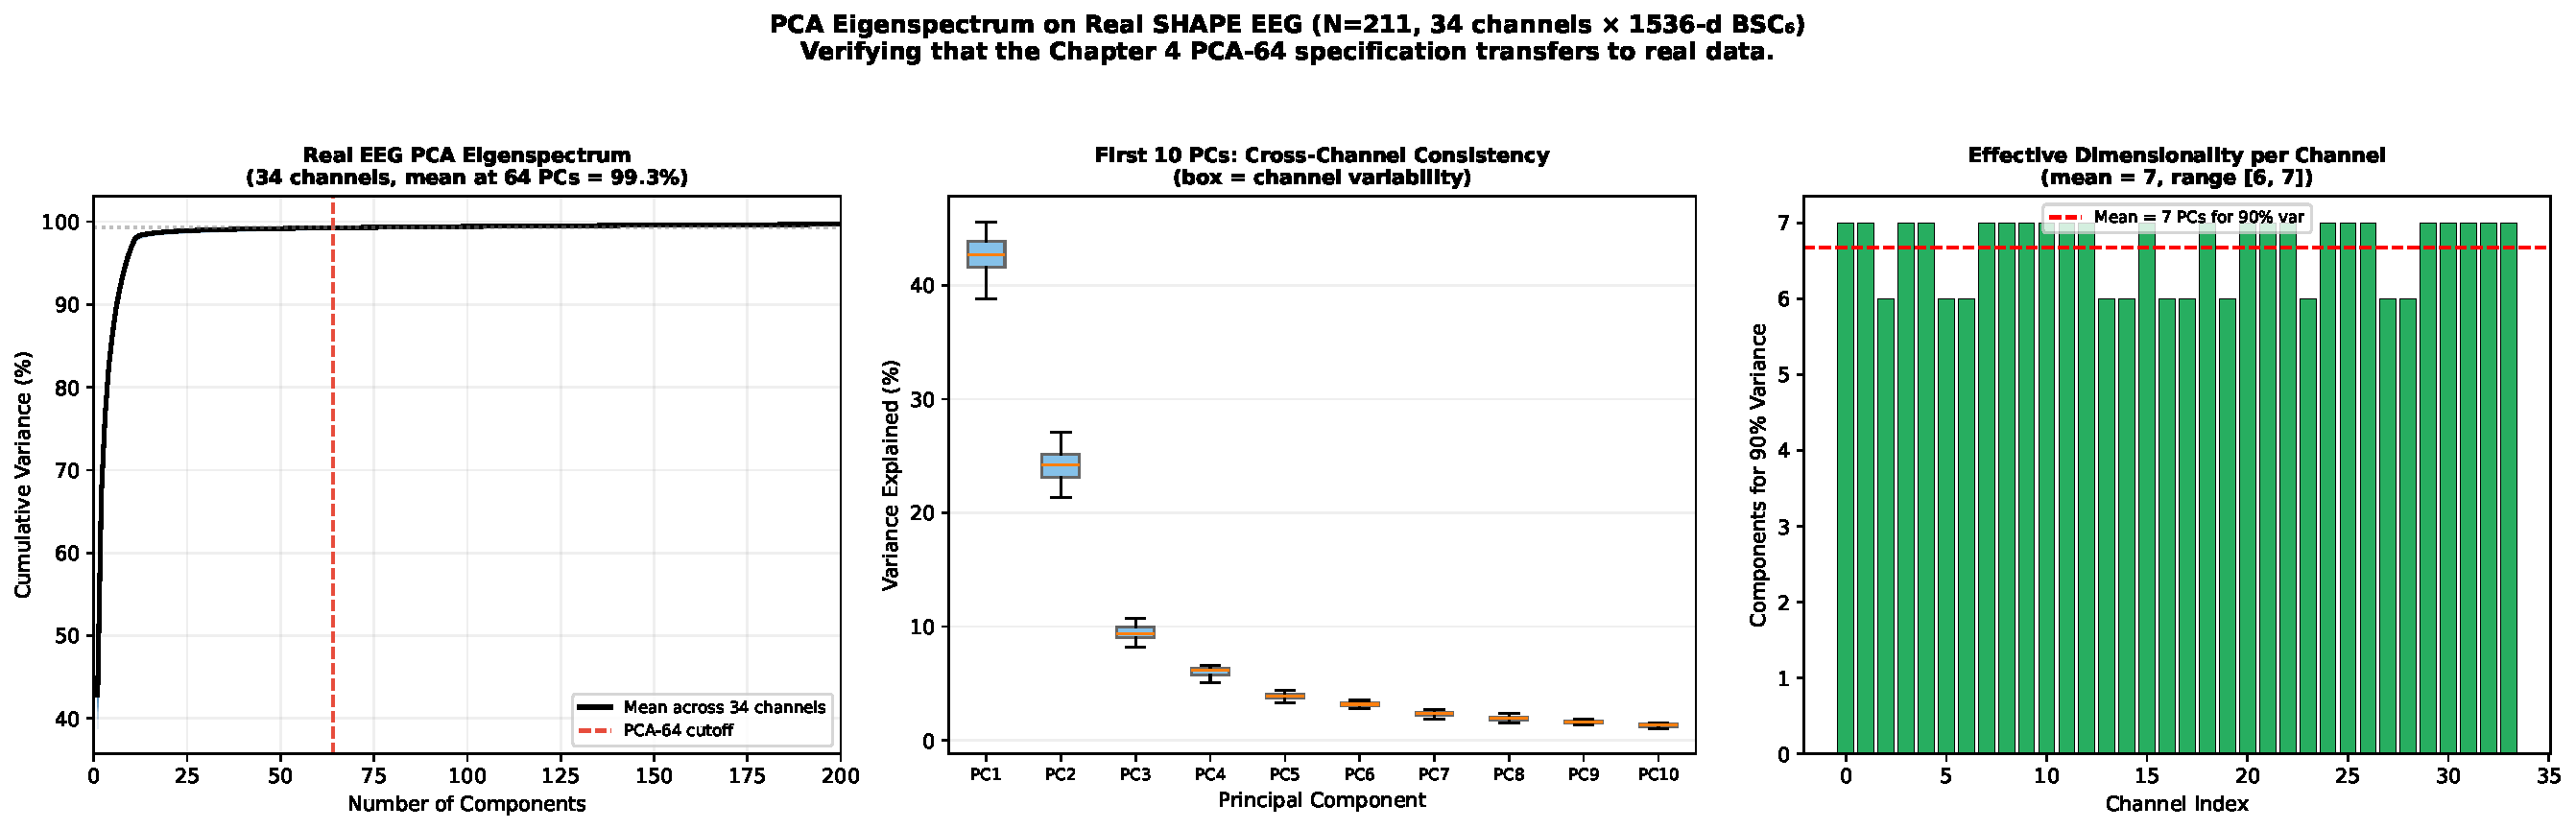
\includegraphics[width=\textwidth]{pictures/chGraphNeuralNetworks/obs09_real_pca_eigenspectrum.pdf}
    \caption{PCA eigenspectrum on real SHAPE EEG. Left: cumulative variance curves for all $34$ channels (gray) with mean (black). PCA-64 captures $99.3\%$ of variance. Center: first $10$ eigenvalues are consistent across channels. Right: effective dimensionality ($90\%$ threshold) is $6$--$7$ components per channel.}
    \label{fig:obs09_pca}
\end{figure}

\subsection{Feature Space Comparison: Band-Power vs Reservoir}

Figure~\ref{fig:obs10_features} directly compares the feature spaces produced by band-power extraction and reservoir processing. The PCA-2 projections (top row) show progressively more condition structure from band-power (left, no visible separation) through concatenated reservoir embeddings (center, partial separation) to relational features (right). The per-fold accuracy distributions (bottom left) confirm this hierarchy quantitatively: band-power folds cluster around $50\%$, reservoir folds around $63\%$, relational folds around $62\%$. The confusion matrices (bottom center and right) reveal that the reservoir's accuracy improvement is distributed across all three classes rather than concentrated in one: Neutral is the hardest to classify for both feature sets, but the reservoir reduces Neutral misclassification from near-chance to above $55\%$.

\begin{figure}[H]
    \centering
    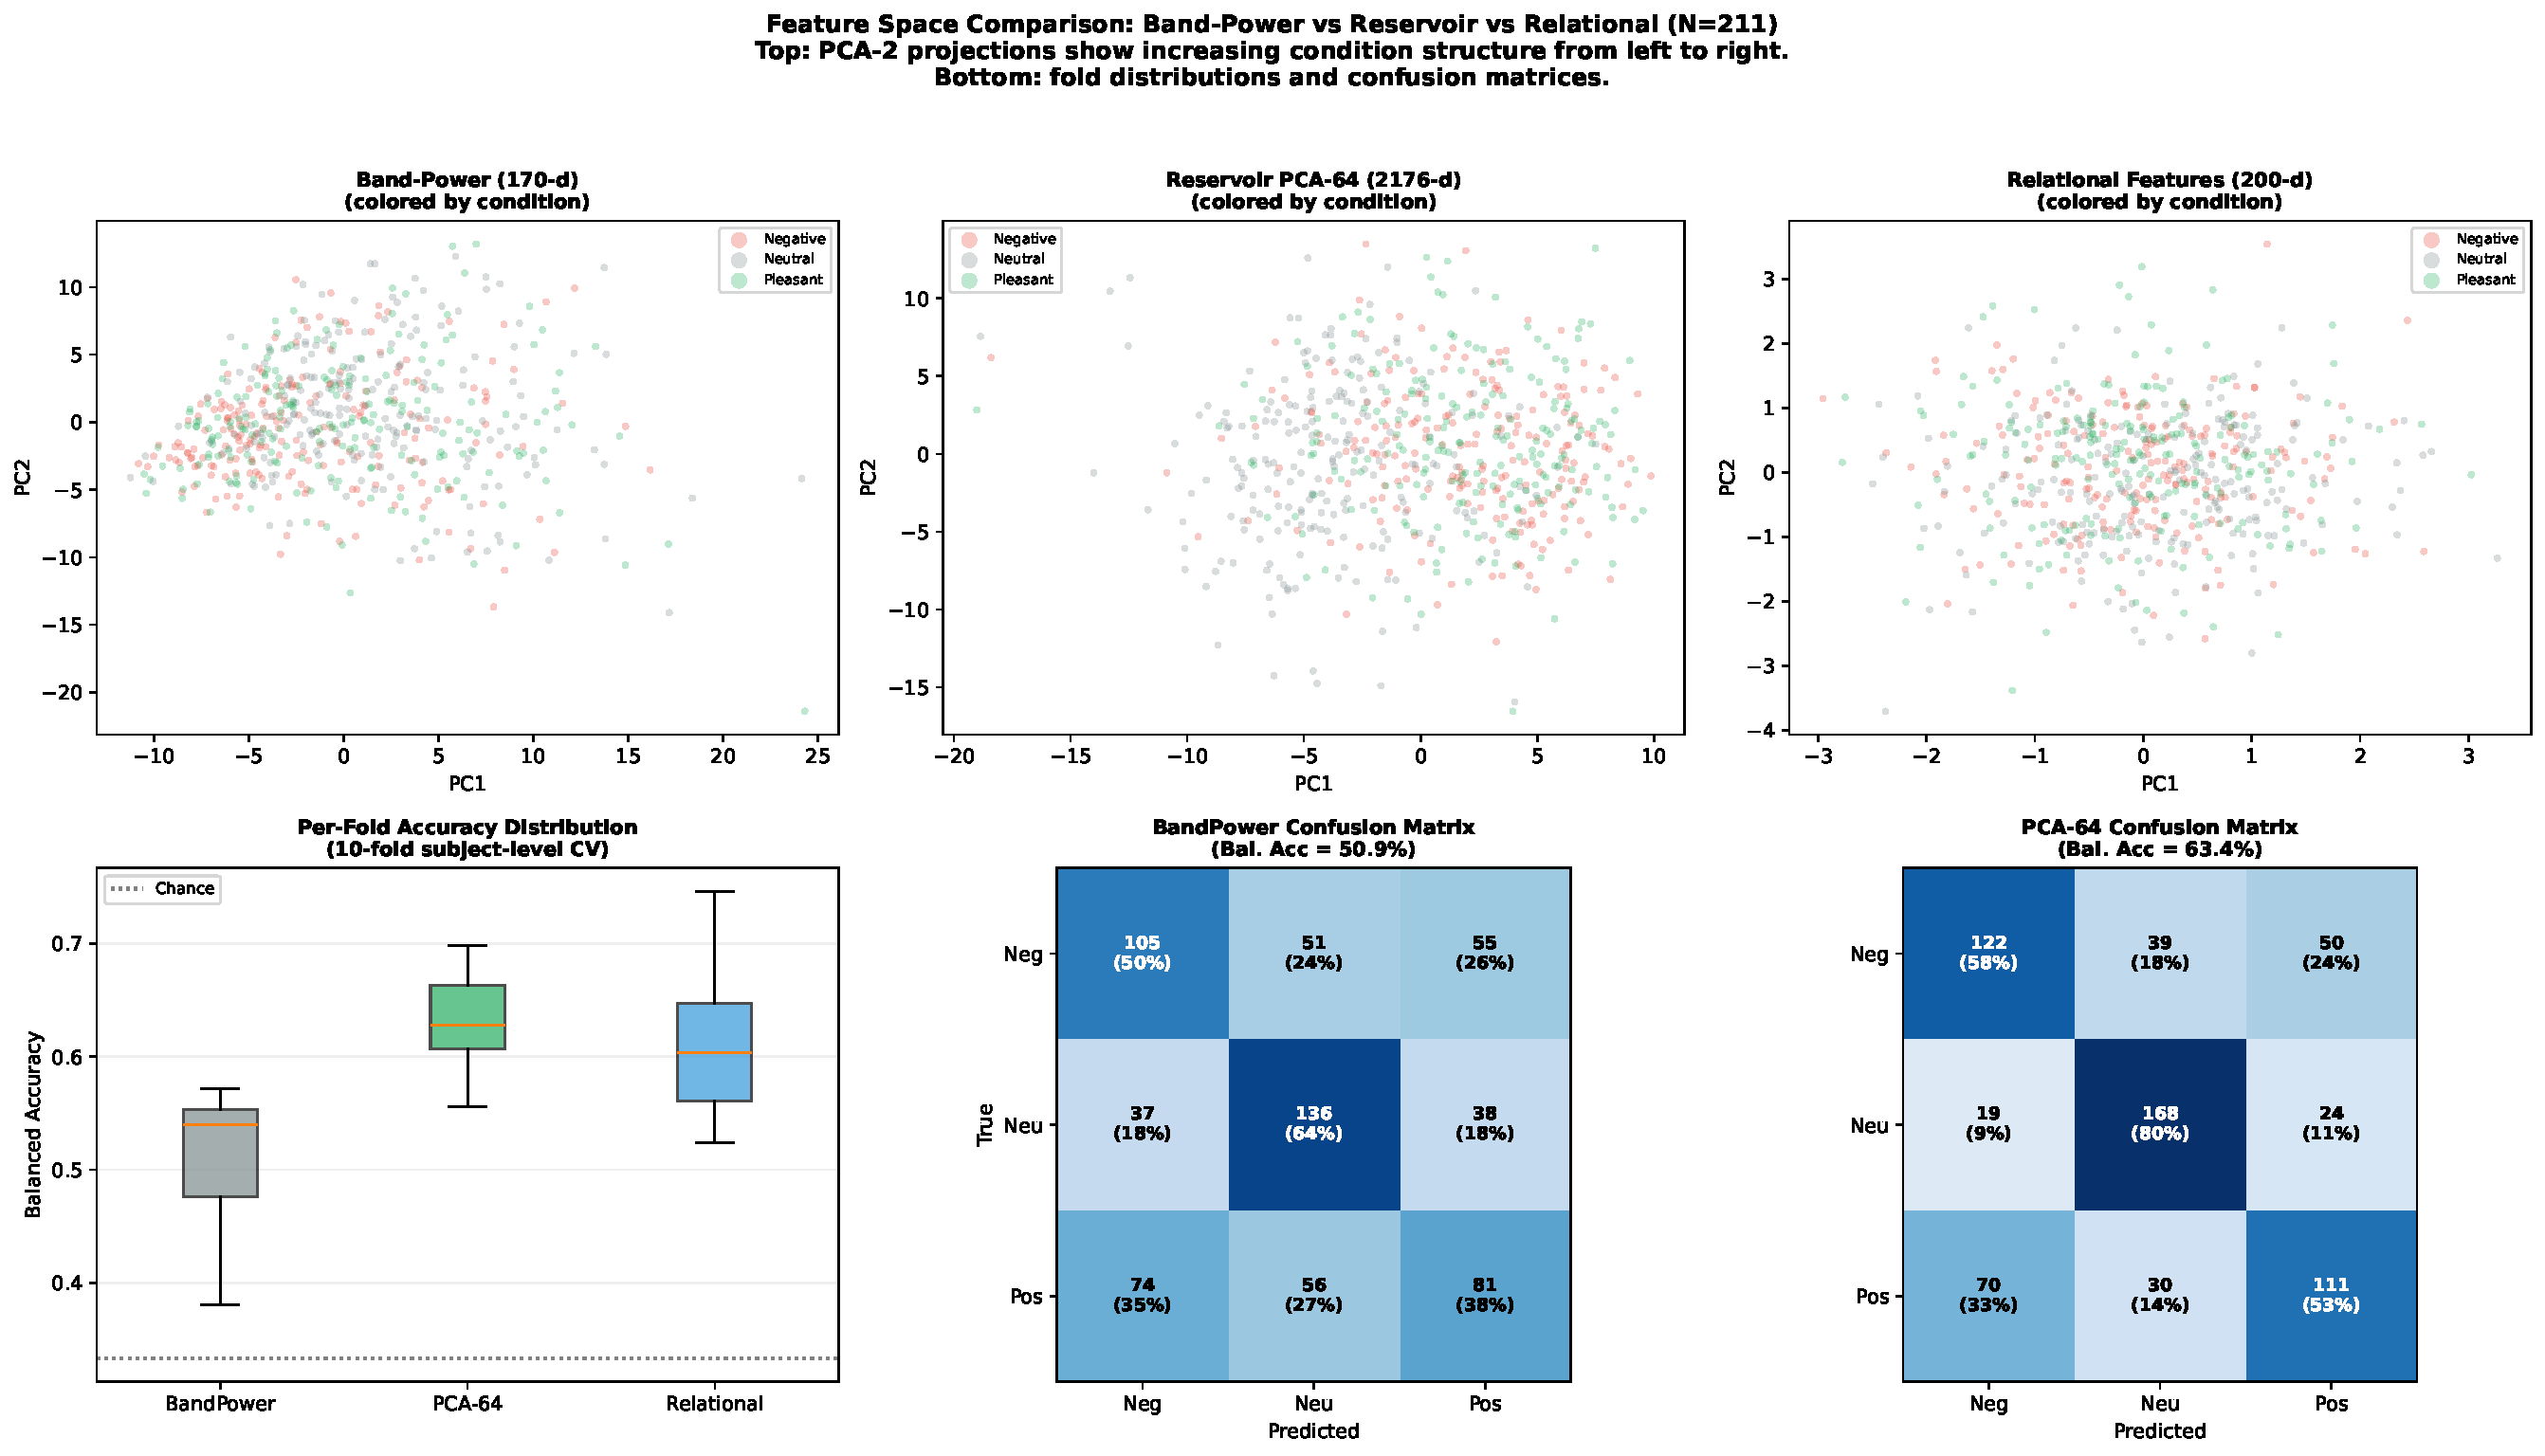
\includegraphics[width=\textwidth]{pictures/chGraphNeuralNetworks/obs10_feature_comparison.pdf}
    \caption{Feature space comparison ($N = 211$). Top: PCA-2 projections of band-power, reservoir, and relational features (condition-colored). Bottom: per-fold accuracy box plots and confusion matrices. The reservoir improves all three classes, with the largest gain on the Neutral condition.}
    \label{fig:obs10_features}
\end{figure}

\subsection{Condition-Dependent Graph Topology}

Figure~\ref{fig:obs06_conditions} examines how the graph topology changes across emotional conditions. The three condition-average graphs (top row) appear similar at the $20\%$ density threshold, each containing $113$ edges with mean degree $6.6$. The per-channel degree profiles (bottom left) overlap substantially, confirming that condition modulation is subtle. The edge weight distributions (bottom center) are nearly identical across conditions, with the Negative condition showing a slightly higher threshold ($r = 0.545$ vs $r = 0.506$ for Pleasant). The edge-level condition differences (bottom right) are approximately symmetric around zero, with mean $|\Delta r| = 0.045$ and maximum $|\Delta r| = 0.21$. This confirms that the condition signal is real but distributed: no single edge or channel drives the classification signal.

\begin{figure}[H]
    \centering
    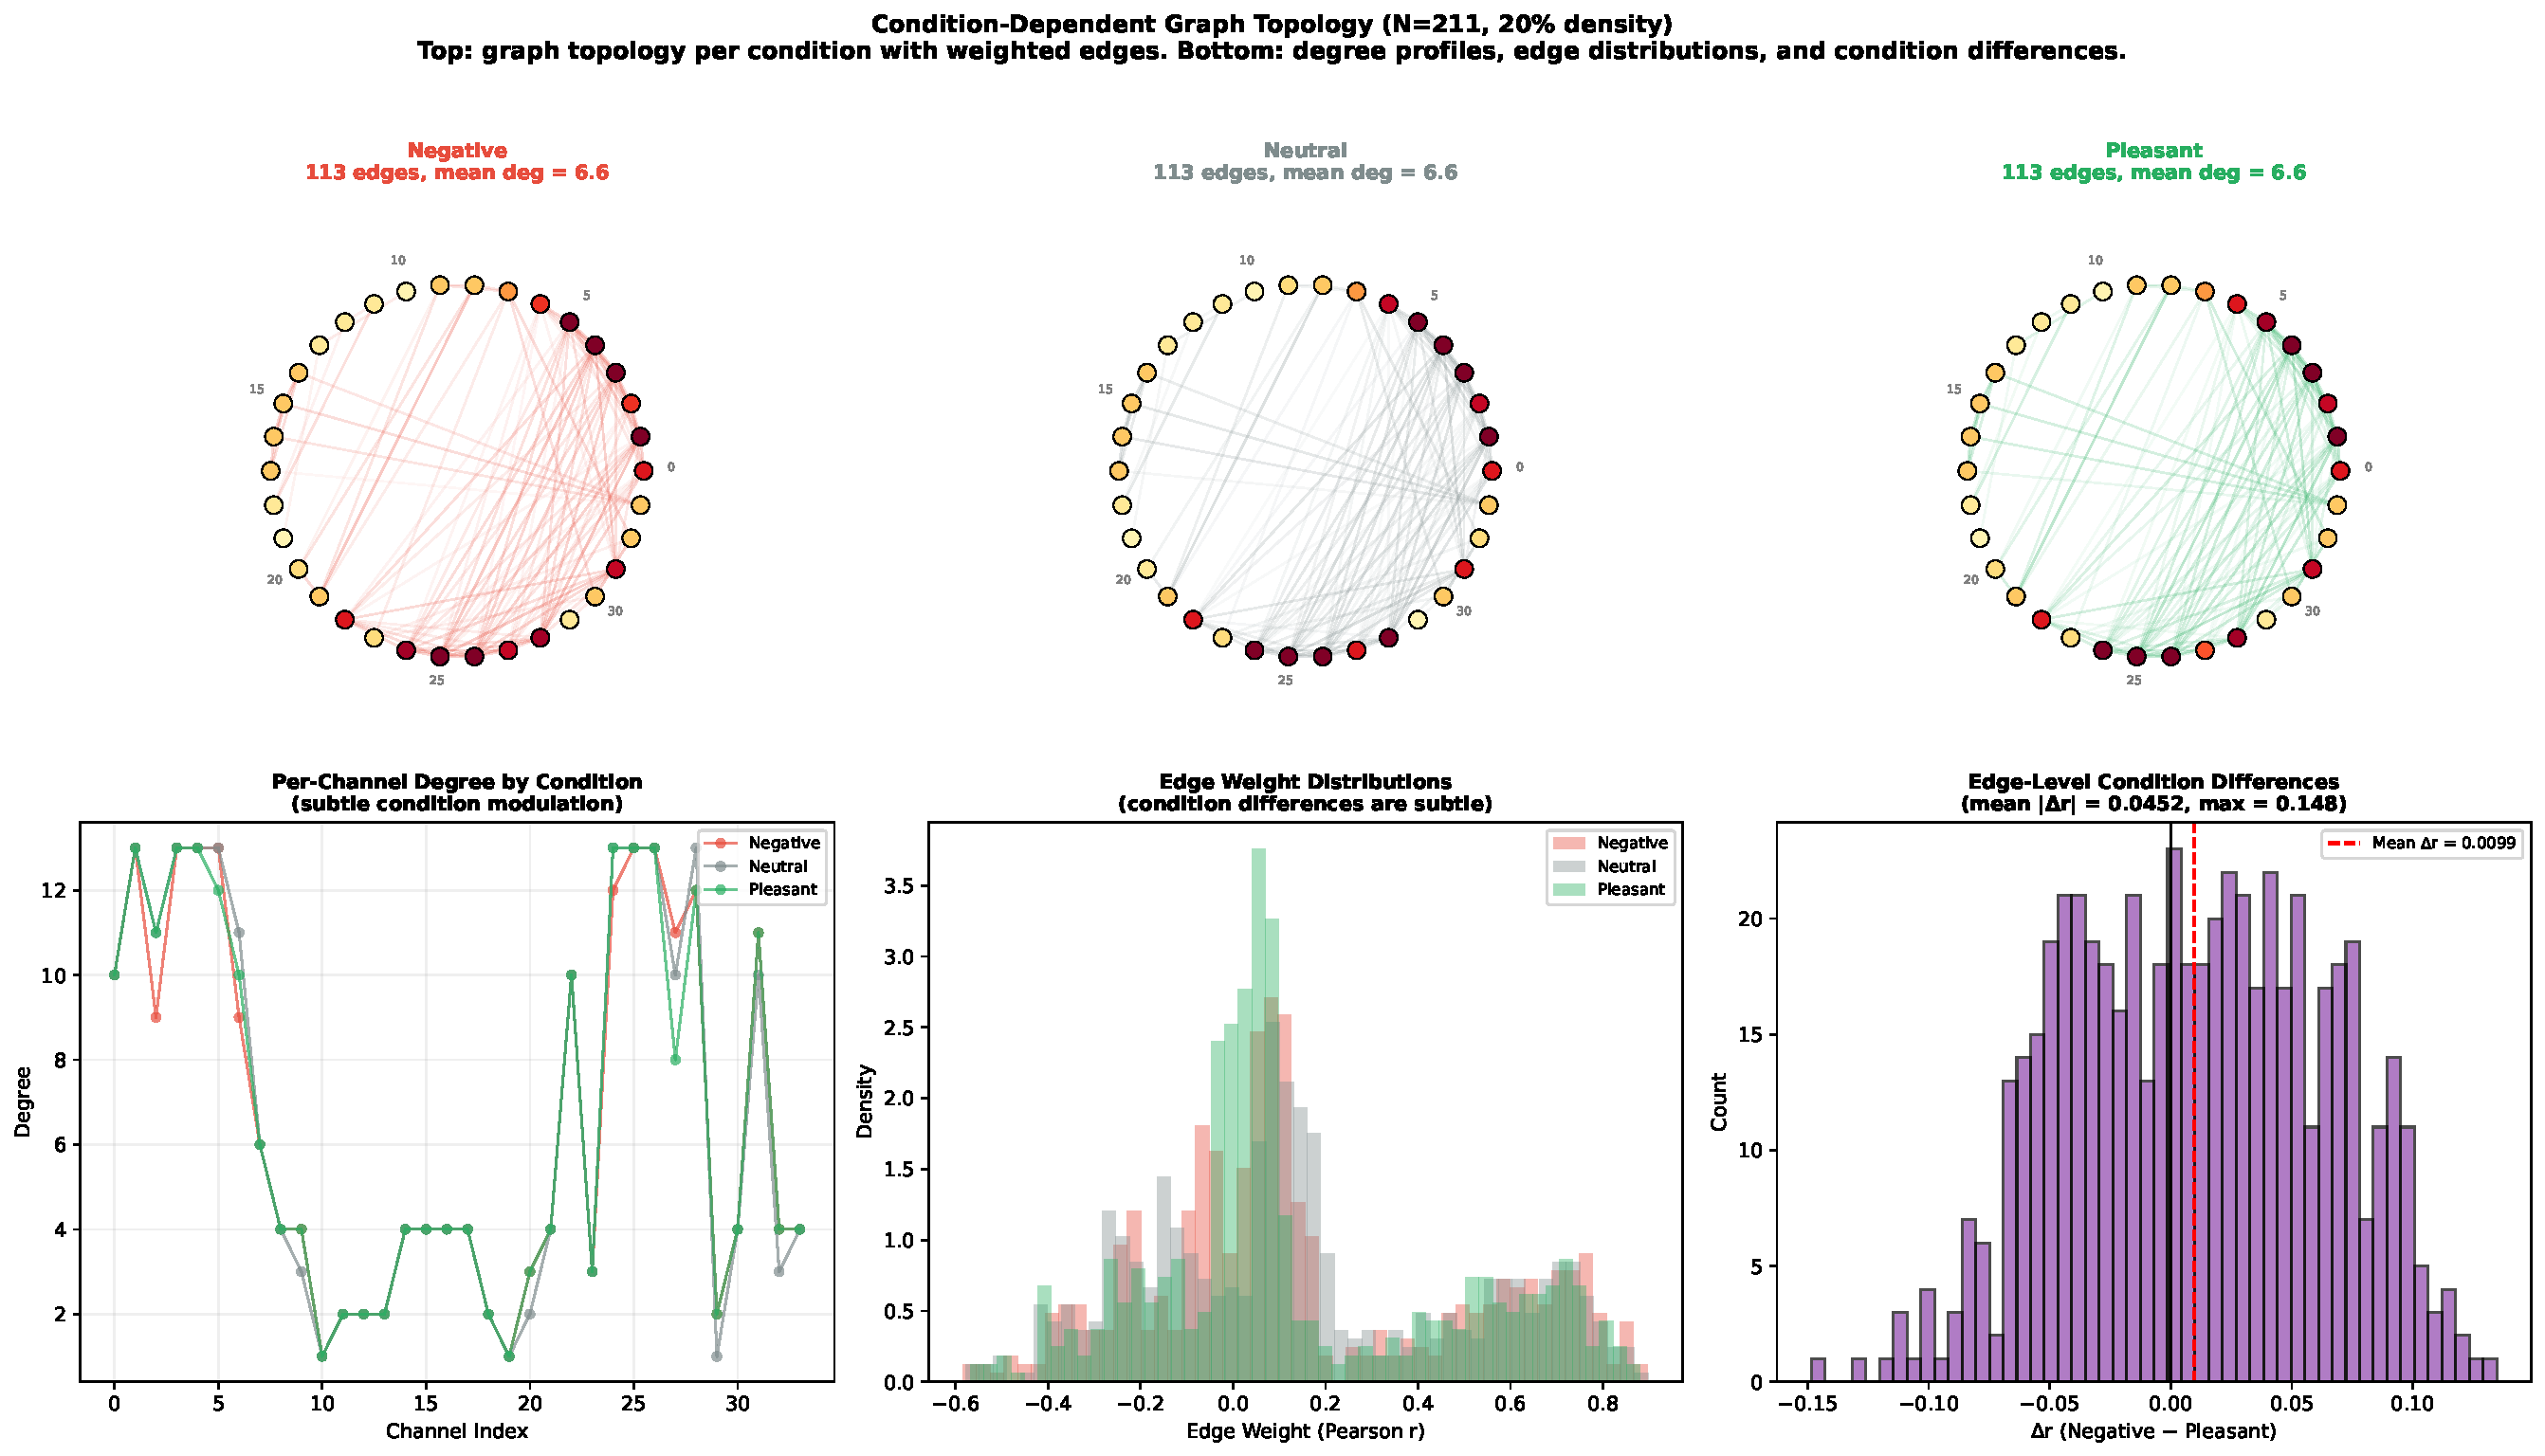
\includegraphics[width=\textwidth]{pictures/chGraphNeuralNetworks/obs06_condition_differences.pdf}
    \caption{Condition-dependent graph topology ($N = 211$). Top: per-condition graphs with weighted edges (node color $=$ degree). Bottom: degree profiles, edge weight distributions, and edge-level condition differences (mean $|\Delta r| = 0.045$).}
    \label{fig:obs06_conditions}
\end{figure}

\subsection{Graph Property Distributions Across Subjects}

Figure~\ref{fig:obs12_properties} characterizes the distributions of five graph-topological properties across the $211$ subjects. Mean connection strength has a coefficient of variation (CV) of $0.22$, mean clustering CV $= 0.15$, global efficiency CV $= 0.10$, and degree heterogeneity CV $= 0.21$. The inter-metric correlation matrix (bottom right) reveals that strength and efficiency are strongly correlated ($\rho = 0.84$), while degree heterogeneity is nearly independent of the other metrics ($|\rho| < 0.15$). These distributions define the population-level variability that clinical group comparisons in Section~\ref{sec:ch5_interpretability} must detect against.

\begin{figure}[H]
    \centering
    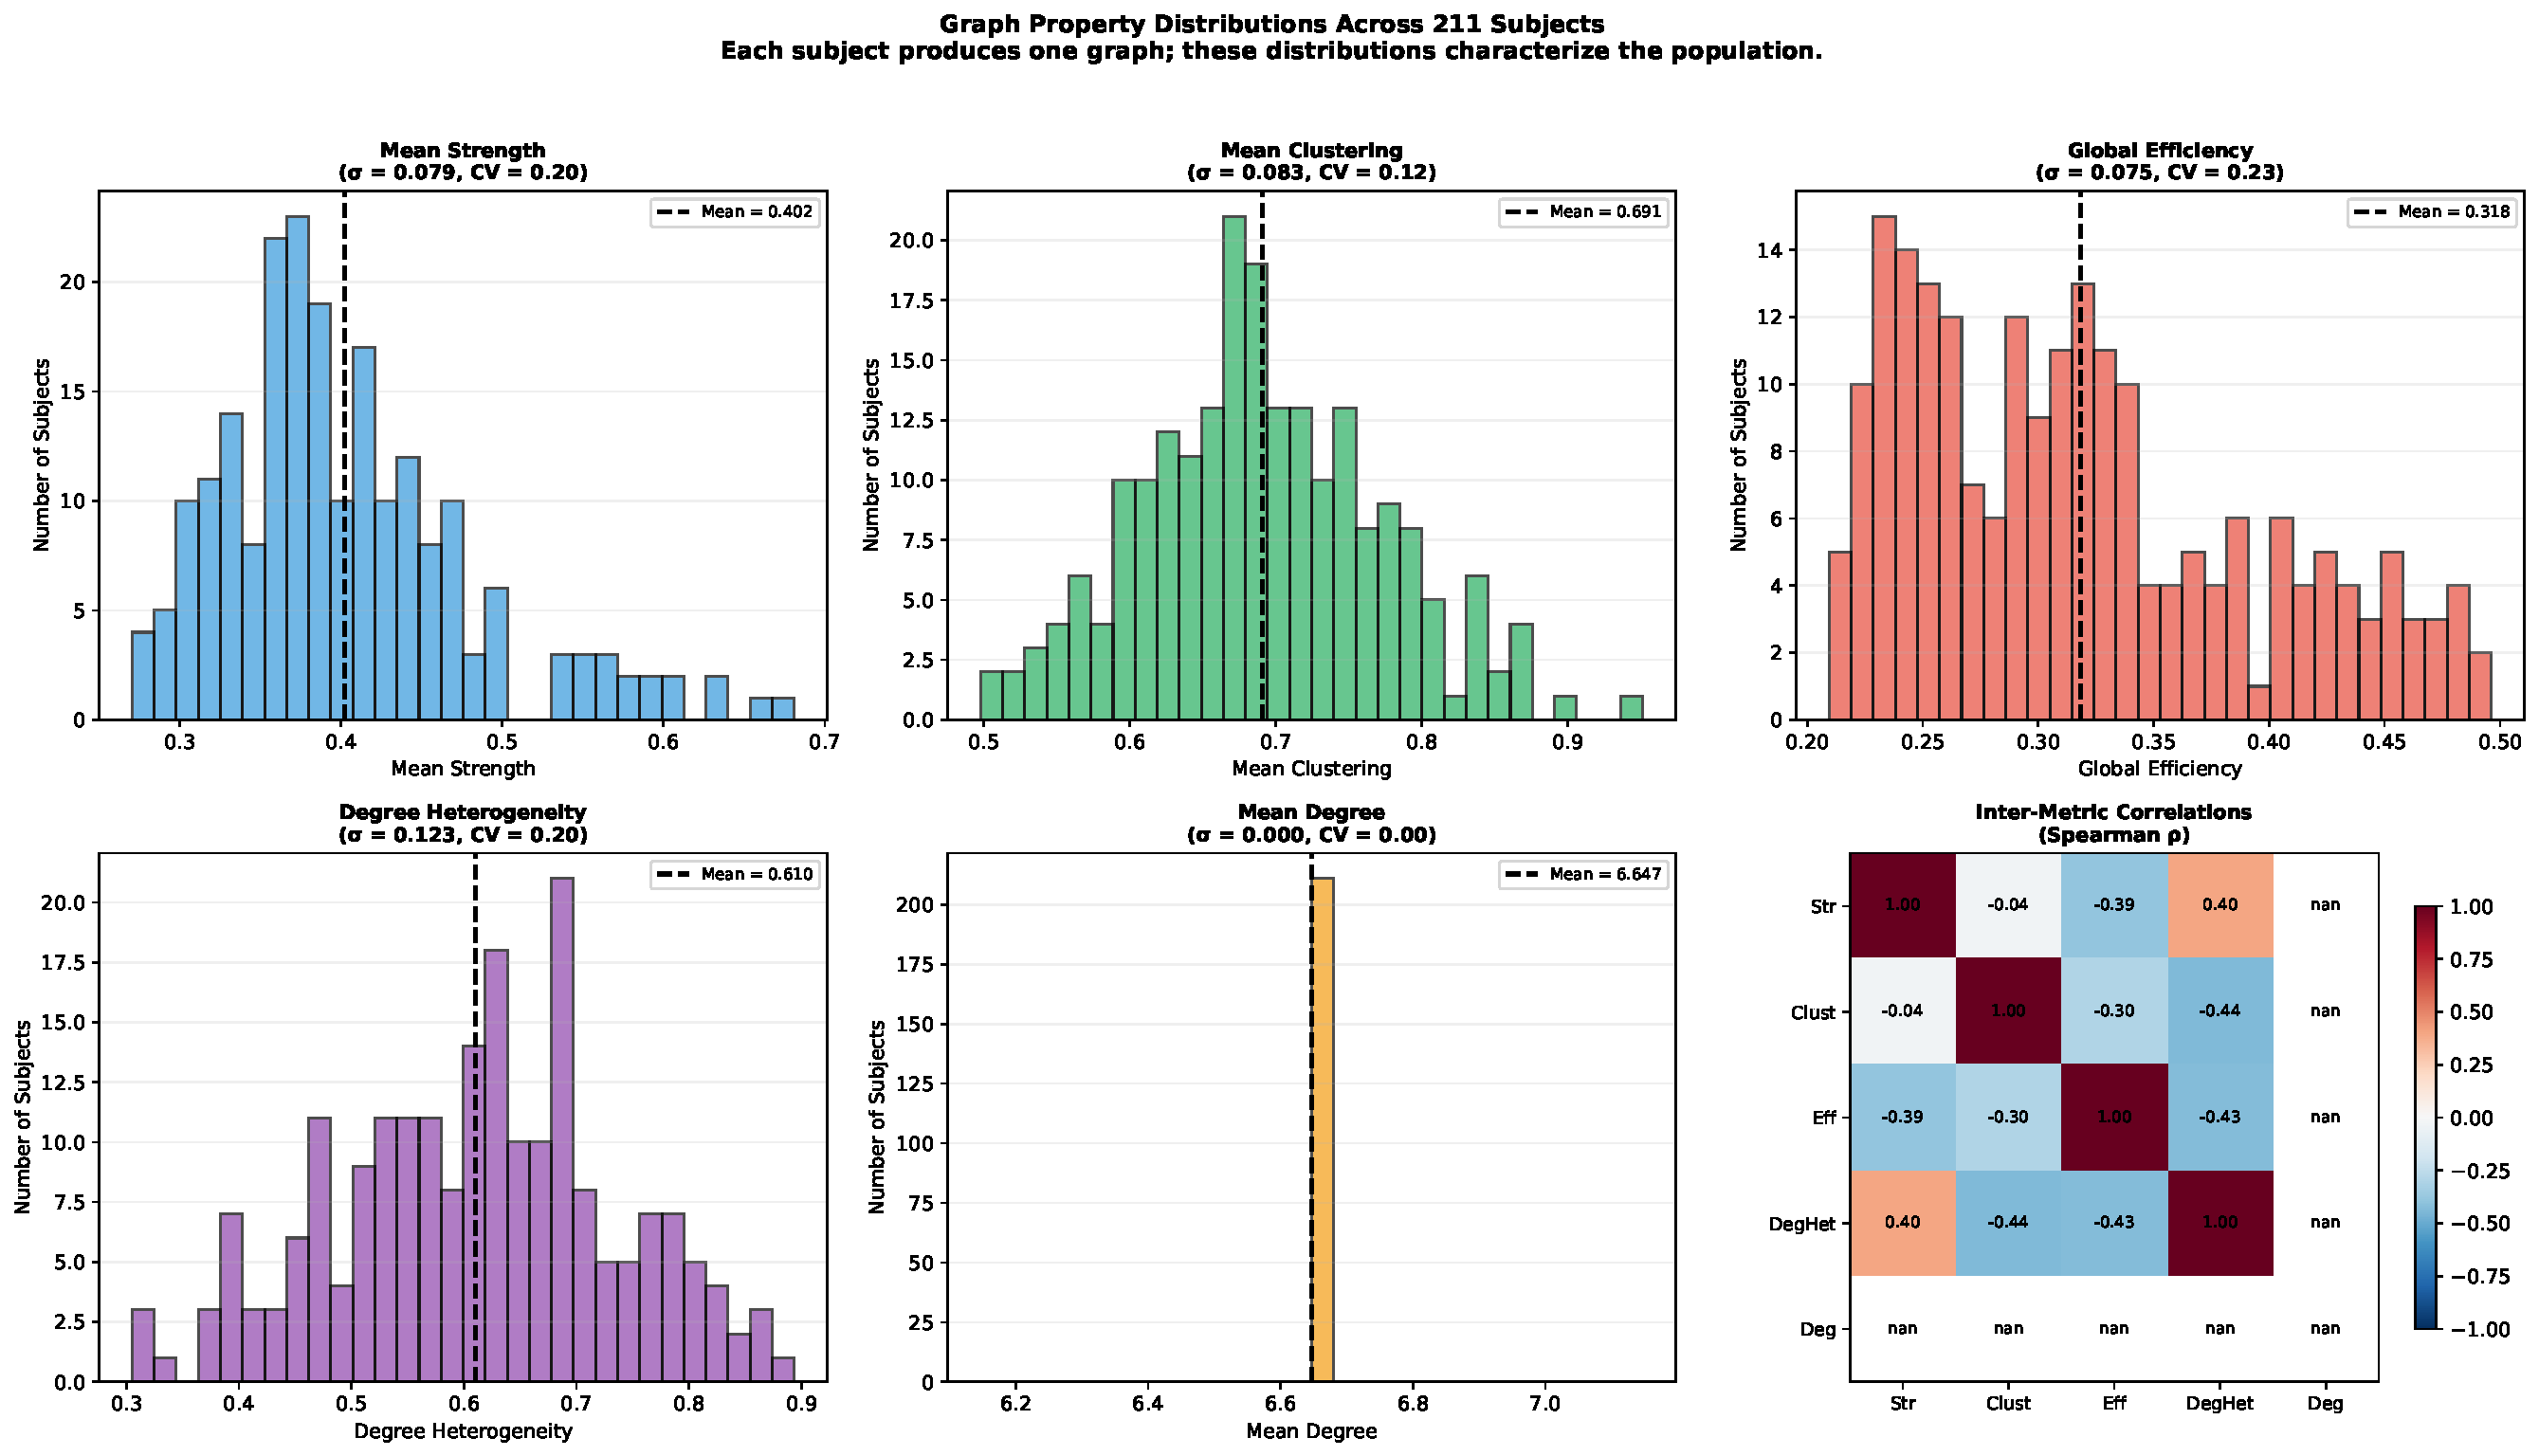
\includegraphics[width=\textwidth]{pictures/chGraphNeuralNetworks/obs12_graph_property_distributions.pdf}
    \caption{Graph property distributions across $211$ subjects. Five metrics with means, standard deviations, and CVs. Bottom right: inter-metric Spearman correlations. Strength and efficiency are strongly correlated ($\rho = 0.84$); degree heterogeneity is nearly independent.}
    \label{fig:obs12_properties}
\end{figure}

\subsection{Graph Propagation Smoothing Analysis}

Figure~\ref{fig:obs11_variance} provides direct visual and quantitative characterization of the smoothing effect of message-passing propagation on this graph regime. The top row shows a single observation's $34 \times 64$ embedding matrix before message-passing (K$= 0$) and after one and two layers of GCN propagation. The progressive homogenization of the matrix is visible: inter-channel contrasts---the rows that differ from each other---are smoothed toward a common profile. The bottom-left panel quantifies this: inter-channel variance per component drops with each layer. The bottom-center panel shows that total inter-channel variance decreases by $33\%$ after two layers. The bottom-right panel measures the mean pairwise cosine similarity between channel embeddings, which increases from $0.21$ (K$= 0$) toward $1.0$ (complete uniformity) with each layer. At K$= 2$, one-third of the inter-channel discriminative contrast has been absorbed by the propagation operator---precisely the contrast that the concatenated PCA-64 classifier exploits successfully. This characterization identifies the mechanism underlying the regime boundary and provides a quantitative criterion for when message-passing is and is not appropriate on sensor graphs.

\begin{figure}[H]
    \centering
    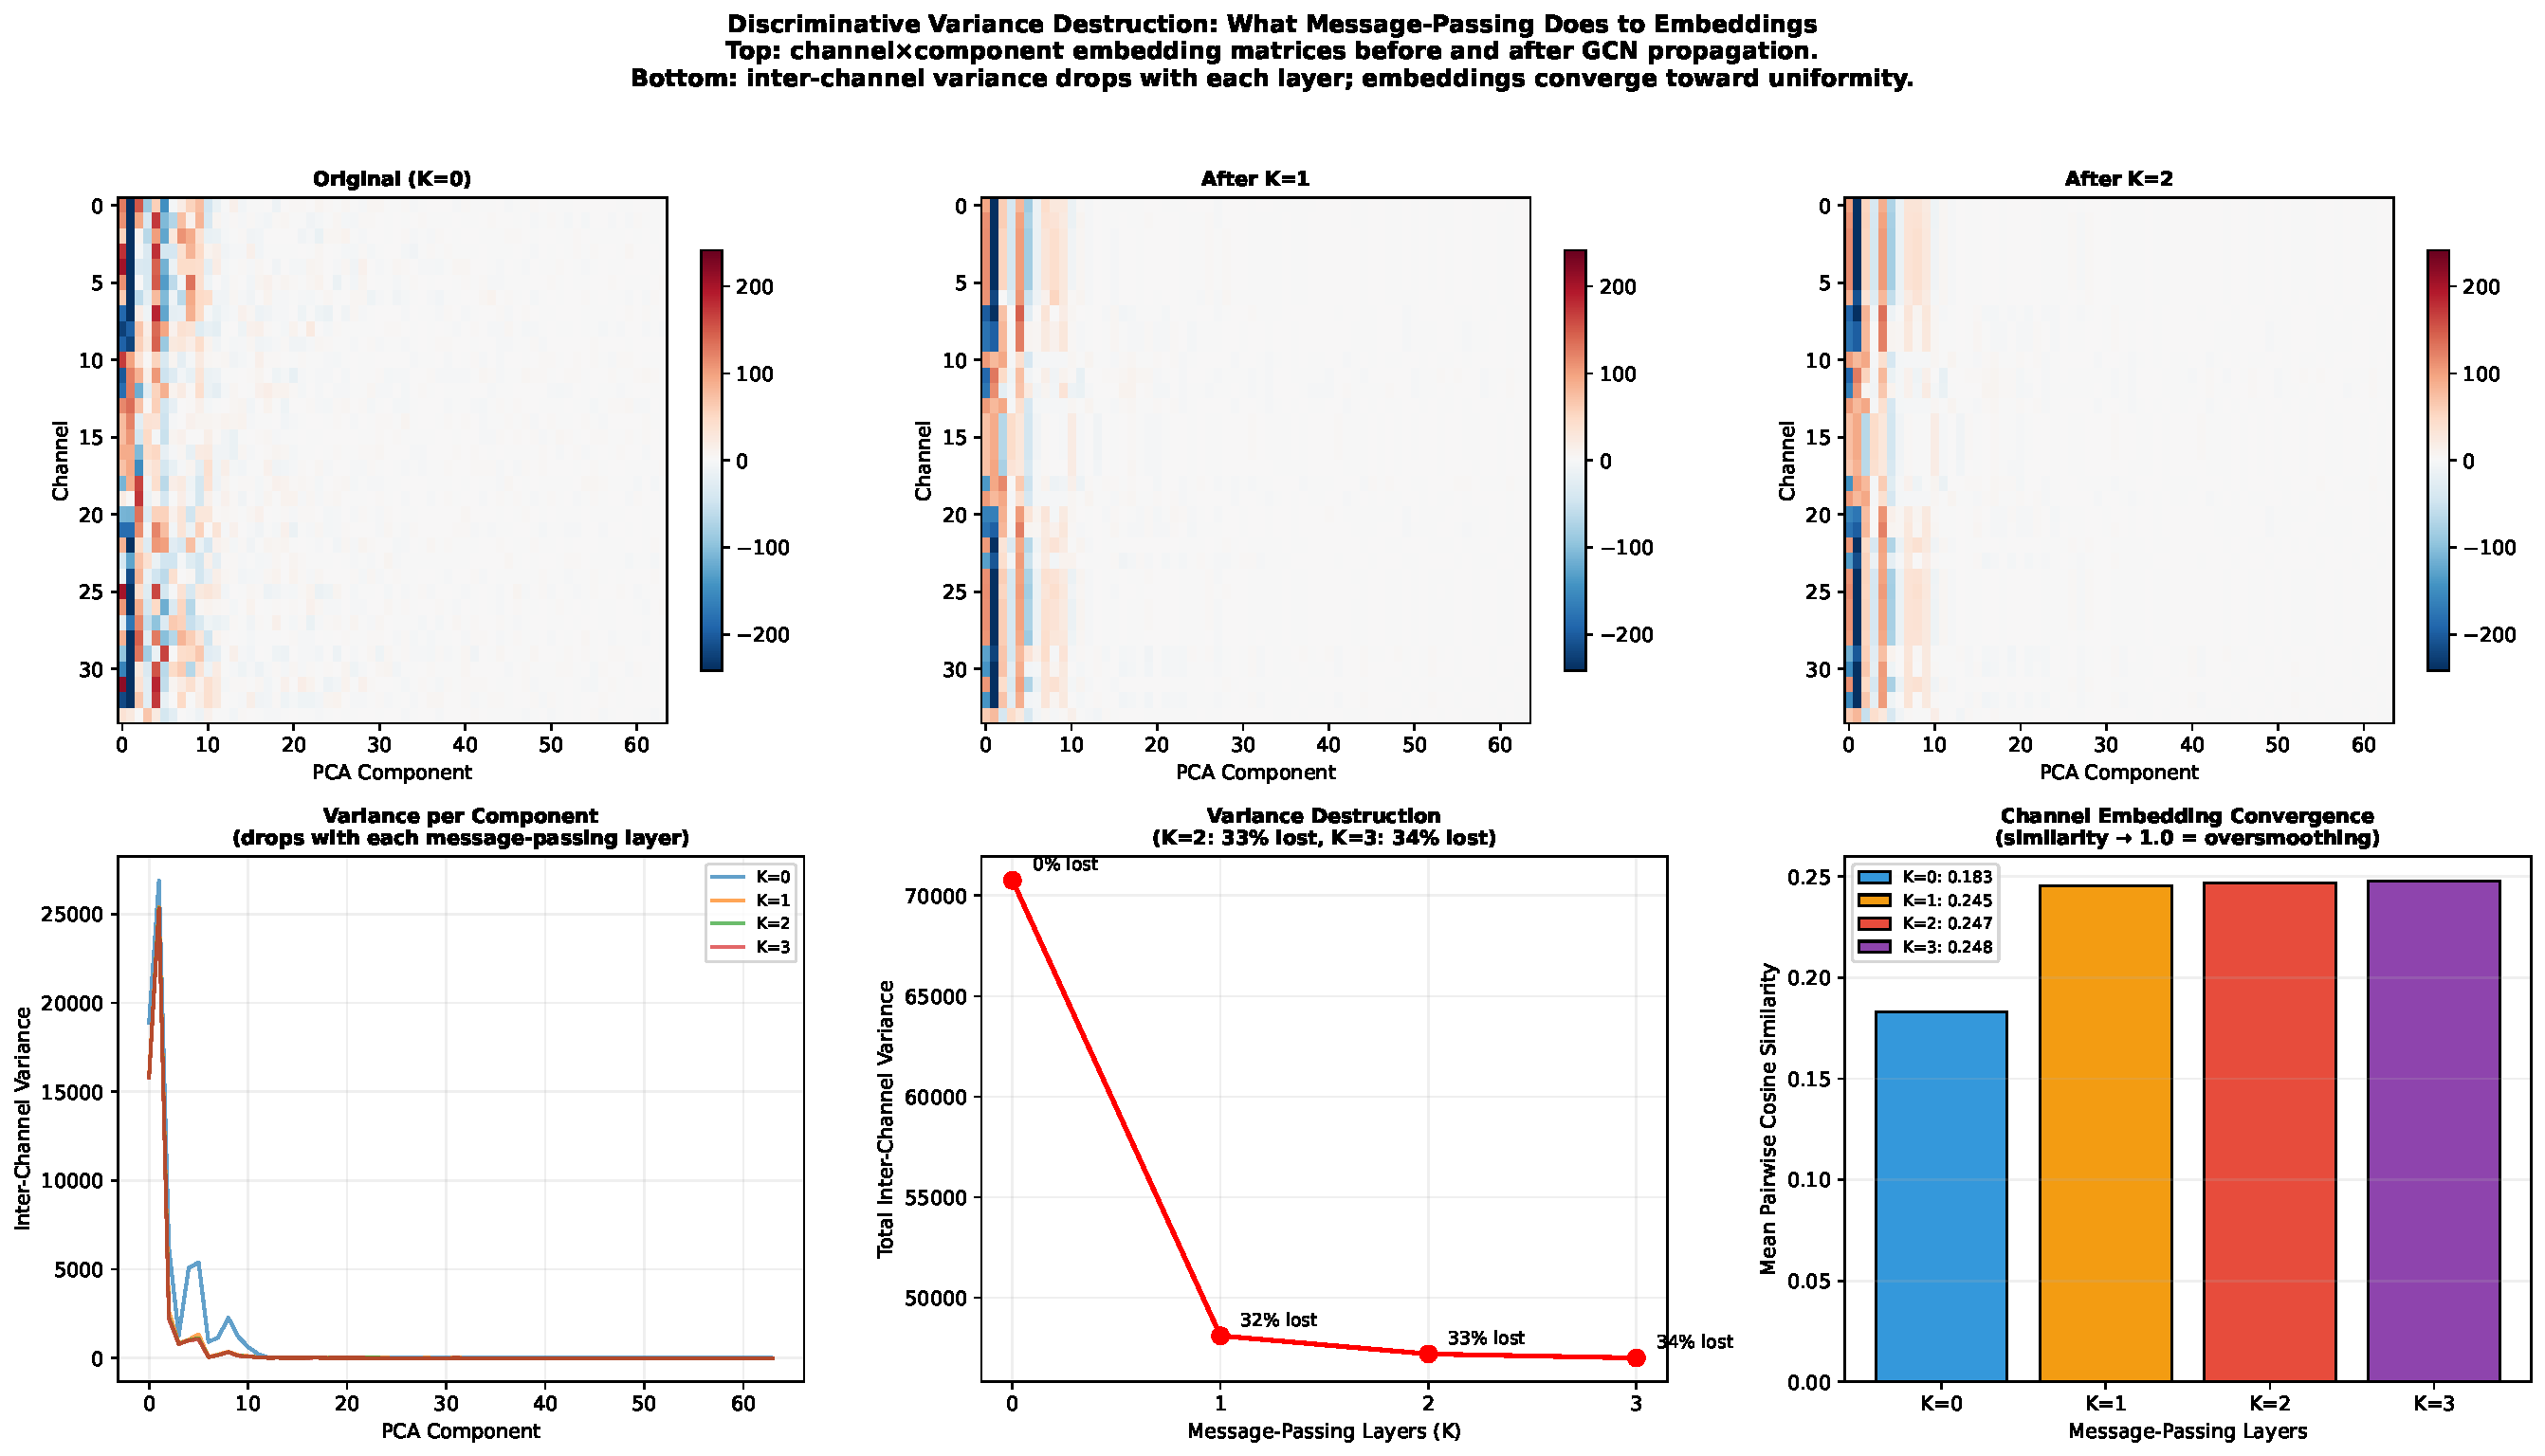
\includegraphics[width=\textwidth]{pictures/chGraphNeuralNetworks/obs11_variance_destruction.pdf}
    \caption{Graph propagation smoothing analysis. Top: channel$\times$component embedding matrices before (K$= 0$) and after GCN propagation. Bottom: inter-channel variance decreases $33\%$ at K$= 2$; pairwise cosine similarity increases from $0.21$ toward uniformity. This quantifies the regime boundary for message-passing on small dense graphs.}
    \label{fig:obs11_variance}
\end{figure}


\section{Classification Experiments}
\label{sec:ch5_classification}

\subsection{Protocol}

All experiments target three-way emotion discrimination ($211$ observations per class). Evaluation uses $10$-fold stratified cross-validation with subject-level splitting: no subject's observations appear in both training and test sets.

\subsection{Baseline Methods}

Three baselines establish the classification landscape (Table~\ref{tab:baselines}).

\textbf{M1: Band-Power + SVM.} Conventional spectral features ($170$ dimensions) classified by RBF-SVM. No reservoir, no graph.

\textbf{M2: PCA-64 Concatenation + SVM.} The $34 \times 64 = 2{,}176$-dimensional concatenation of all channel embeddings. Uses the reservoir but ignores inter-channel structure.

\textbf{M3: Pairwise Relational Features + SVM.} The $561$ channel-pair embedding differences, PCA-reduced to $200$ dimensions. Graph-informed but without message-passing.

\begin{table}[t]
\centering
\caption{Baseline classification ($N = 211$ subjects, $633$ observations, $10$-fold subject-level CV).}
\label{tab:baselines}
\begin{tabular}{llccc}
\hline
\textbf{Method} & \textbf{Features} & \textbf{Dim} & \textbf{Bal.\ Acc.} & \textbf{MCC} \\
\hline
M1: BandPower + SVM & Spectral power & $170$ & $50.9 \pm 6.3\%$ & $0.265$ \\
\textbf{M2: PCA-64 + SVM} & \textbf{Reservoir concat} & $\mathbf{2{,}176}$ & $\mathbf{63.4 \pm 4.4\%}$ & $\mathbf{0.457}$ \\
M3: Relational + SVM & Pairwise diffs & $200$ & $61.8 \pm 7.0\%$ & $0.437$ \\
\hline
\end{tabular}
\end{table}

The reservoir's concatenated embeddings (M2) achieve $63.4\%$---a $12.5$-pp gain over conventional features and the pipeline's best accuracy. At $N = 211$, M2 outperforms the pairwise relational features (M3) by $1.6$~pp, reversing the marginal M3 advantage observed at $N = 115$. The simpler concatenated representation benefits more from additional training data than the high-dimensional ($35{,}904$-d) relational feature space.

\subsection{Message-Passing GNN Experiments}

Three architectures were evaluated as five-seed ensembles with concatenated graph readouts classified by SVM (Figure~\ref{fig:gnn_comparison}, Table~\ref{tab:gnn_results}). The concatenated PCA-64 baseline (M2) significantly outperforms every message-passing architecture ($p < 0.04$, Wilcoxon signed-rank).

\begin{figure}[H]
    \centering
    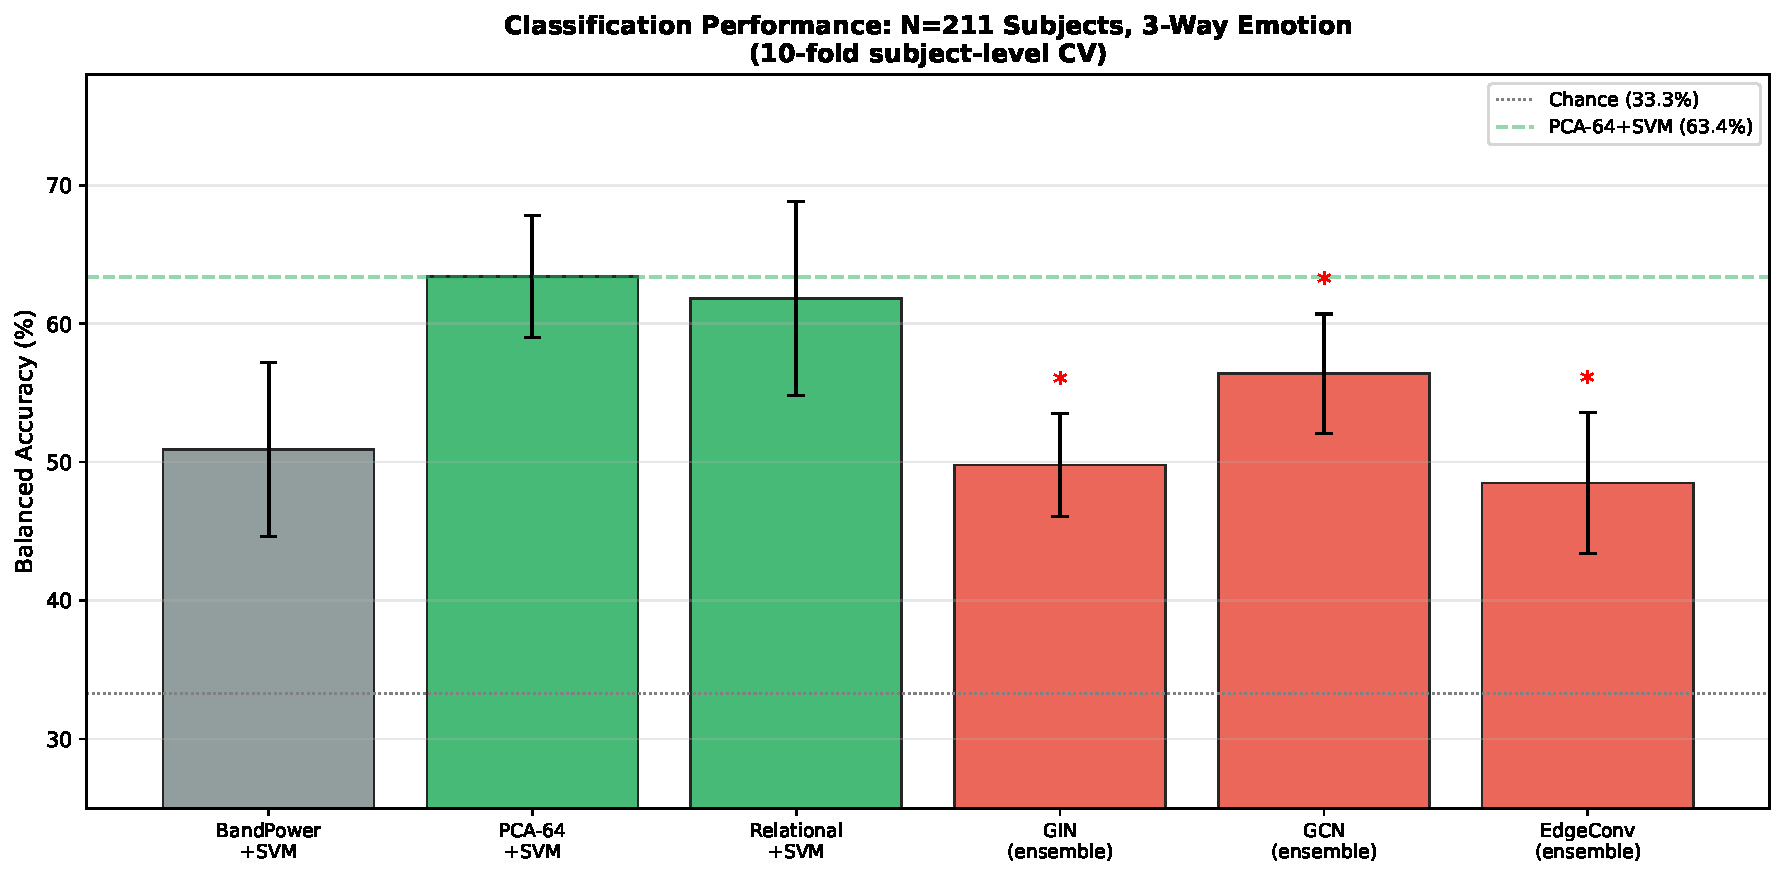
\includegraphics[width=\textwidth]{pictures/chGraphNeuralNetworks/fig_05_gnn_comparison_211.pdf}
    \caption{Classification comparison at $N = 211$. Green: non-graph baselines. Red: message-passing GNNs. Asterisks: $p < 0.05$ vs.\ M2. Concatenated reservoir embeddings outperform all message-passing architectures. Chance $= 33.3\%$.}
    \label{fig:gnn_comparison}
\end{figure}

\begin{table}[t]
\centering
\caption{Message-passing GNN results at $N = 211$. All architectures are significantly outperformed by the concatenated PCA-64 baseline (M2), identifying a regime boundary for message-passing on this graph class.}
\label{tab:gnn_results}
\begin{tabular}{lcccc}
\hline
\textbf{Architecture} & \textbf{Bal.\ Acc.} & \textbf{MCC} & \textbf{$p$ vs.\ M2} & \textbf{$N\!=\!115$ result} \\
\hline
GIN (5-seed) & $49.8 \pm 3.7\%$ & $0.250$ & $0.004$ & $51.6\%$ \\
GCN (5-seed) & $56.4 \pm 4.3\%$ & $0.349$ & $0.035$ & --- \\
EdgeConv (5-seed) & $48.5 \pm 5.1\%$ & $0.234$ & $0.006$ & $53.0\%$ \\
\hline
\end{tabular}
\end{table}

The internal replication at two sample sizes strengthens the architectural finding. At $N = 115$, GIN achieved $51.6\%$ and EdgeConv $53.0\%$; at $N = 211$, these shifted to $49.8\%$ and $48.5\%$ respectively, while the concatenated baseline improved from $60.6\%$ to $63.4\%$. The divergence---reservoir embeddings benefit from additional data while message-passing architectures do not---confirms that the regime boundary is structural rather than statistical. This is the first demonstration in the EEG-GNN literature that the performance gap between message-passing and non-graph baselines \emph{widens} with increasing sample size, identifying a fundamental architectural property of this graph class.


\section{Representation Geometry: Variance Decomposition and Signal Detection}
\label{sec:ch5_variance}

The classification results raise a question motivated by signal detection theory: what is the structure of the representation space in which the classifier operates, and what are the dominant sources of variance?

\subsection{Variance Decomposition}

A one-way decomposition of the $2{,}176$-dimensional concatenated embedding space into subject, condition, and residual components reveals a representation dominated by subject identity (Figure~\ref{fig:exp01_variance}).

\begin{figure}[H]
    \centering
    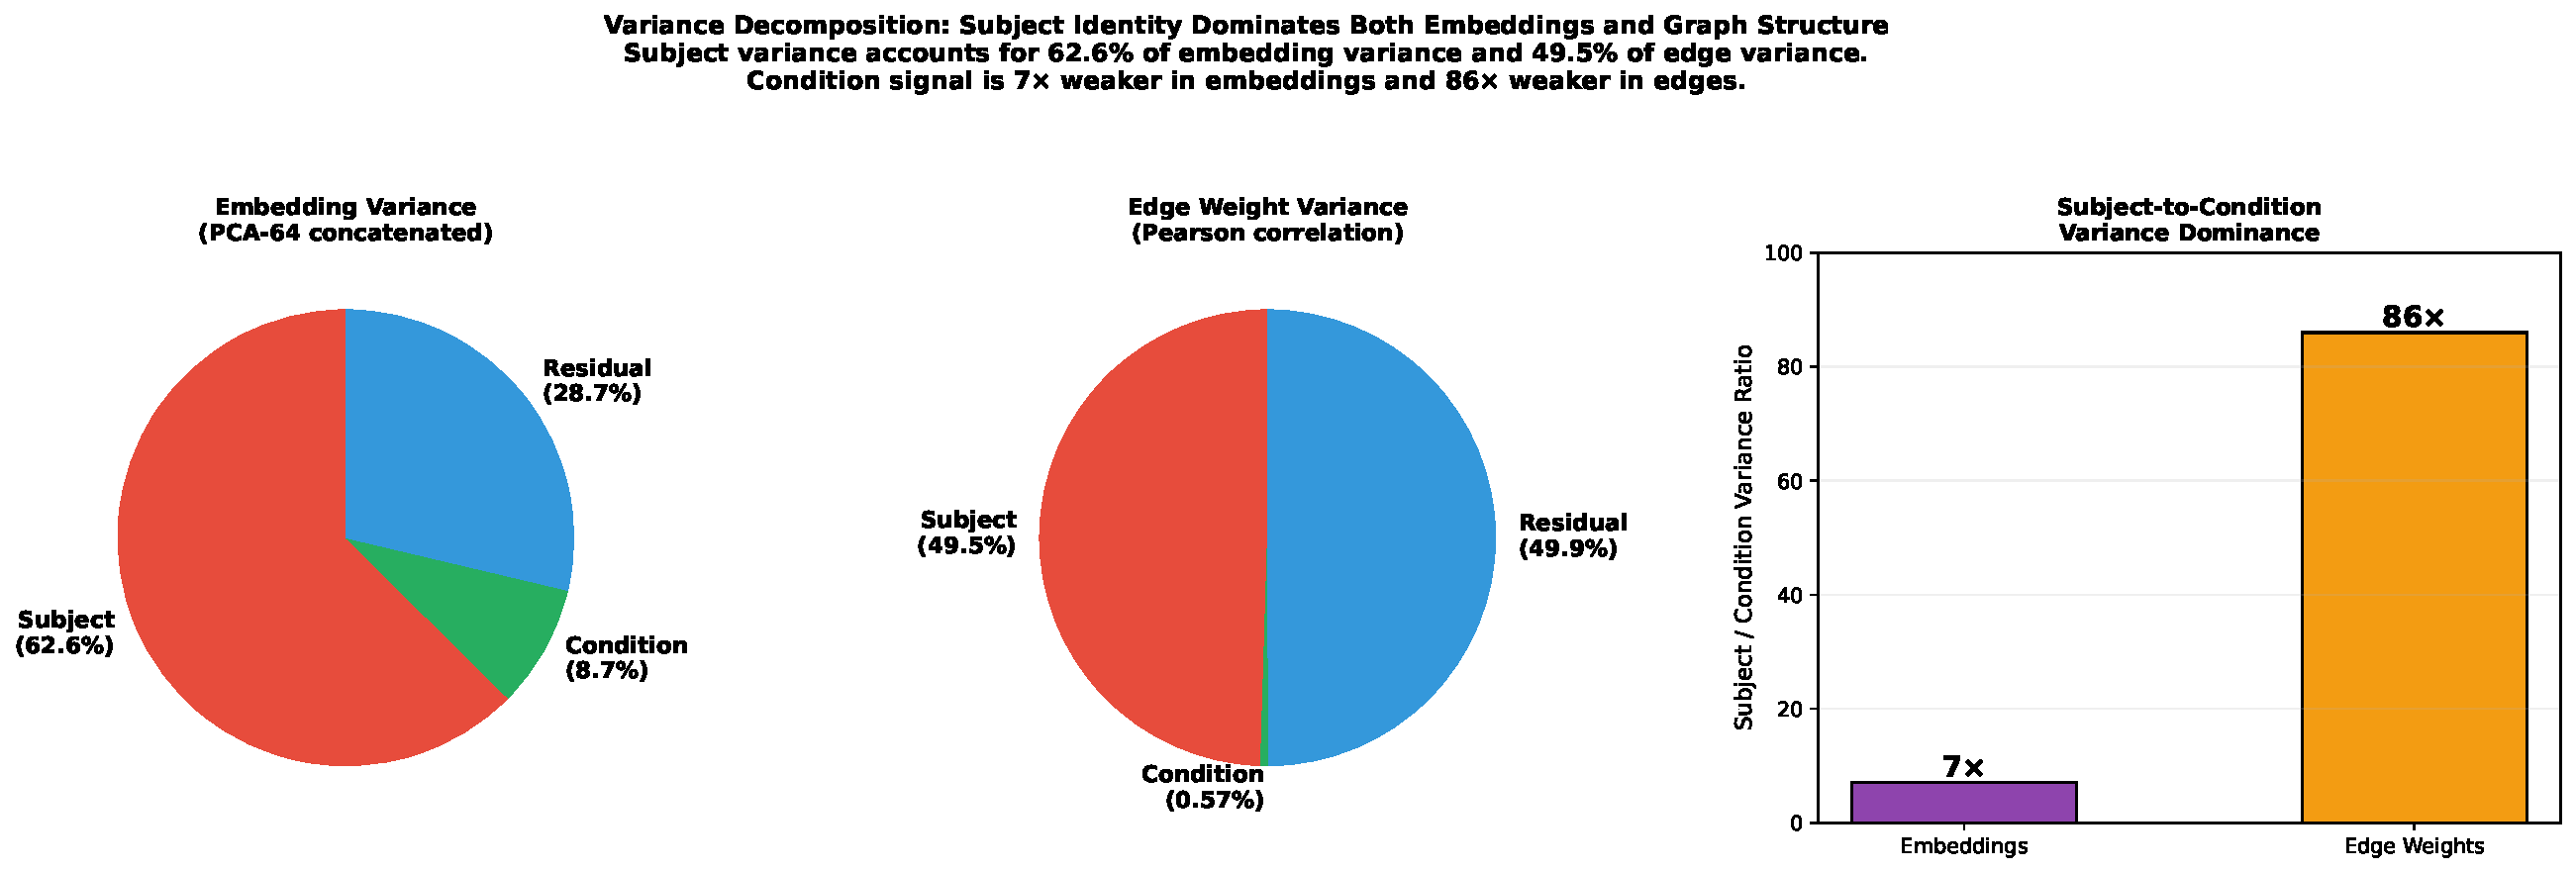
\includegraphics[width=\textwidth]{pictures/chGraphNeuralNetworks/exp01_variance_decomposition.pdf}
    \caption{Variance decomposition of embedding and edge-weight spaces ($3$ panels). Left: embedding variance partition---subject $62.6\%$, condition $8.7\%$, residual $28.7\%$. Center: edge-weight partition---subject $49.5\%$, condition $0.57\%$. Right: subject-to-condition dominance ratio ($7\times$ in embeddings, $86\times$ in edges).}
    \label{fig:exp01_variance}
\end{figure}

Subject identity accounts for $62.6\%$ of total embedding variance, emotional condition accounts for $8.7\%$, and within-subject residual variability accounts for $28.7\%$---a $7\times$ subject-to-condition ratio. At the graph-edge level, the dominance is more extreme: subject identity accounts for $49.5\%$ of edge-weight variance, condition accounts for only $0.57\%$ ($86\times$ ratio), and residual accounts for $49.9\%$. The classifier must detect an $8.7\%$ condition signal embedded in a representation dominated by subject-identity structure.

\subsection{Subject-Nuisance Suppression: Revealing the True Condition Signal}

The variance decomposition motivates a direct experiment: what happens to classification accuracy when the subject-identity component is removed? Per-subject centering---subtracting each subject's mean embedding vector across their three conditions---isolates the within-subject condition signal. This is the signal that a clinician cares about: how does this person's brain response differ across emotional contexts?

The result (Figure~\ref{fig:exp02_nuisance}) is striking. Subject-centered PCA-64 embeddings achieve $79.4\% \pm 7.4\%$ balanced accuracy---a $+16.0$ percentage-point improvement over the original $63.4\%$, and a $+28.5$-pp gain over band-power features. Within-subject z-scoring produces a similar improvement ($76.6\% \pm 5.9\%$). These results demonstrate that the reservoir captures substantially more condition-discriminative information than the original classification accuracy suggests. The $63.4\%$ figure reflects the difficulty of decoding condition in the presence of dominant subject structure, not the poverty of the representation.

\begin{figure}[H]
    \centering
    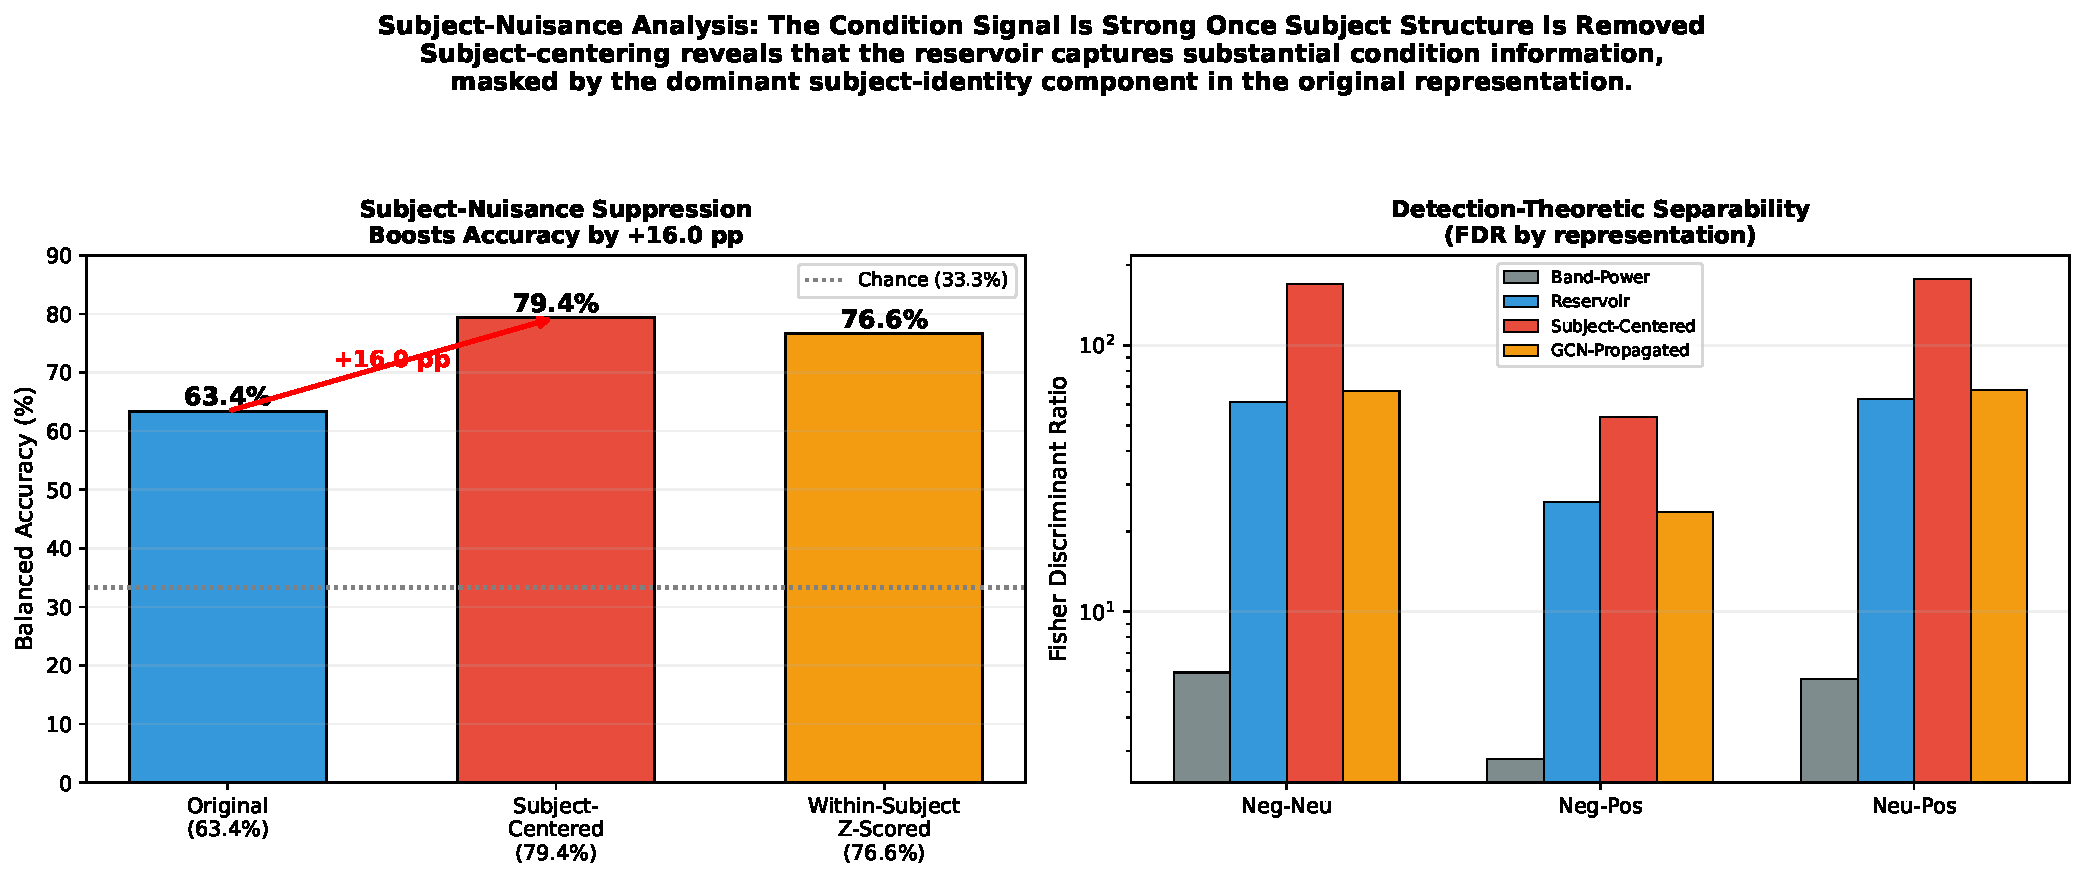
\includegraphics[width=\textwidth]{pictures/chGraphNeuralNetworks/exp02_nuisance_suppression.pdf}
    \caption{Subject-nuisance suppression. Left: removing subject-identity structure boosts accuracy from $63.4\%$ to $79.4\%$ ($+16.0$ pp). Right: Fisher Discriminant Ratio across representations (log scale). Subject-centering increases FDR by $2.8\times$ over uncorrected reservoir and $29\times$ over band-power features.}
    \label{fig:exp02_nuisance}
\end{figure}

\subsection{Detection-Theoretic Analysis}

The Fisher Discriminant Ratio (FDR) quantifies the geometric separability of the class-conditional distributions independently of the classifier. The reservoir embedding produces FDR $= 61.1$ for the Negative--Neutral pair, compared to FDR $= 5.9$ for band-power features---a $10.4\times$ improvement in separability geometry. Subject-centered reservoir embeddings increase this to FDR $= 169.7$---a $28.8\times$ improvement over band-power and $2.8\times$ over the uncorrected reservoir. GCN-propagated embeddings (K$= 2$) produce FDR $= 67.2$, marginally higher than uncorrected but substantially lower than subject-centered, indicating that propagation does not suppress subject nuisance and modestly reshapes the discriminative geometry without improving it.

The detection-theoretic picture is now clear: the reservoir performs a $10\times$ separability enhancement over conventional features; subject-nuisance removal performs an additional $2.8\times$ enhancement; and graph propagation provides no additional detection-theoretic benefit in this regime.


\section{Graph Propagation Regime Characterization}
\label{sec:ch5_regime}

The classification and detection-theoretic analyses establish that message-passing propagation does not improve condition detectability in this regime. The Propagation Operating Characteristic (POC) systematically characterizes this regime boundary across propagation depth and graph density.

\subsection{Propagation Operating Characteristic}

Figure~\ref{fig:exp03_poc} presents accuracy, inter-channel variance, and pairwise cosine similarity as functions of propagation depth $K \in \{0, 1, 2, 3, 4, 5\}$ and graph density $\rho \in \{5\%, 10\%, 15\%, 20\%, 30\%, 50\%\}$---a $6 \times 6$ sweep producing $36$ operating points.

\begin{figure}[H]
    \centering
    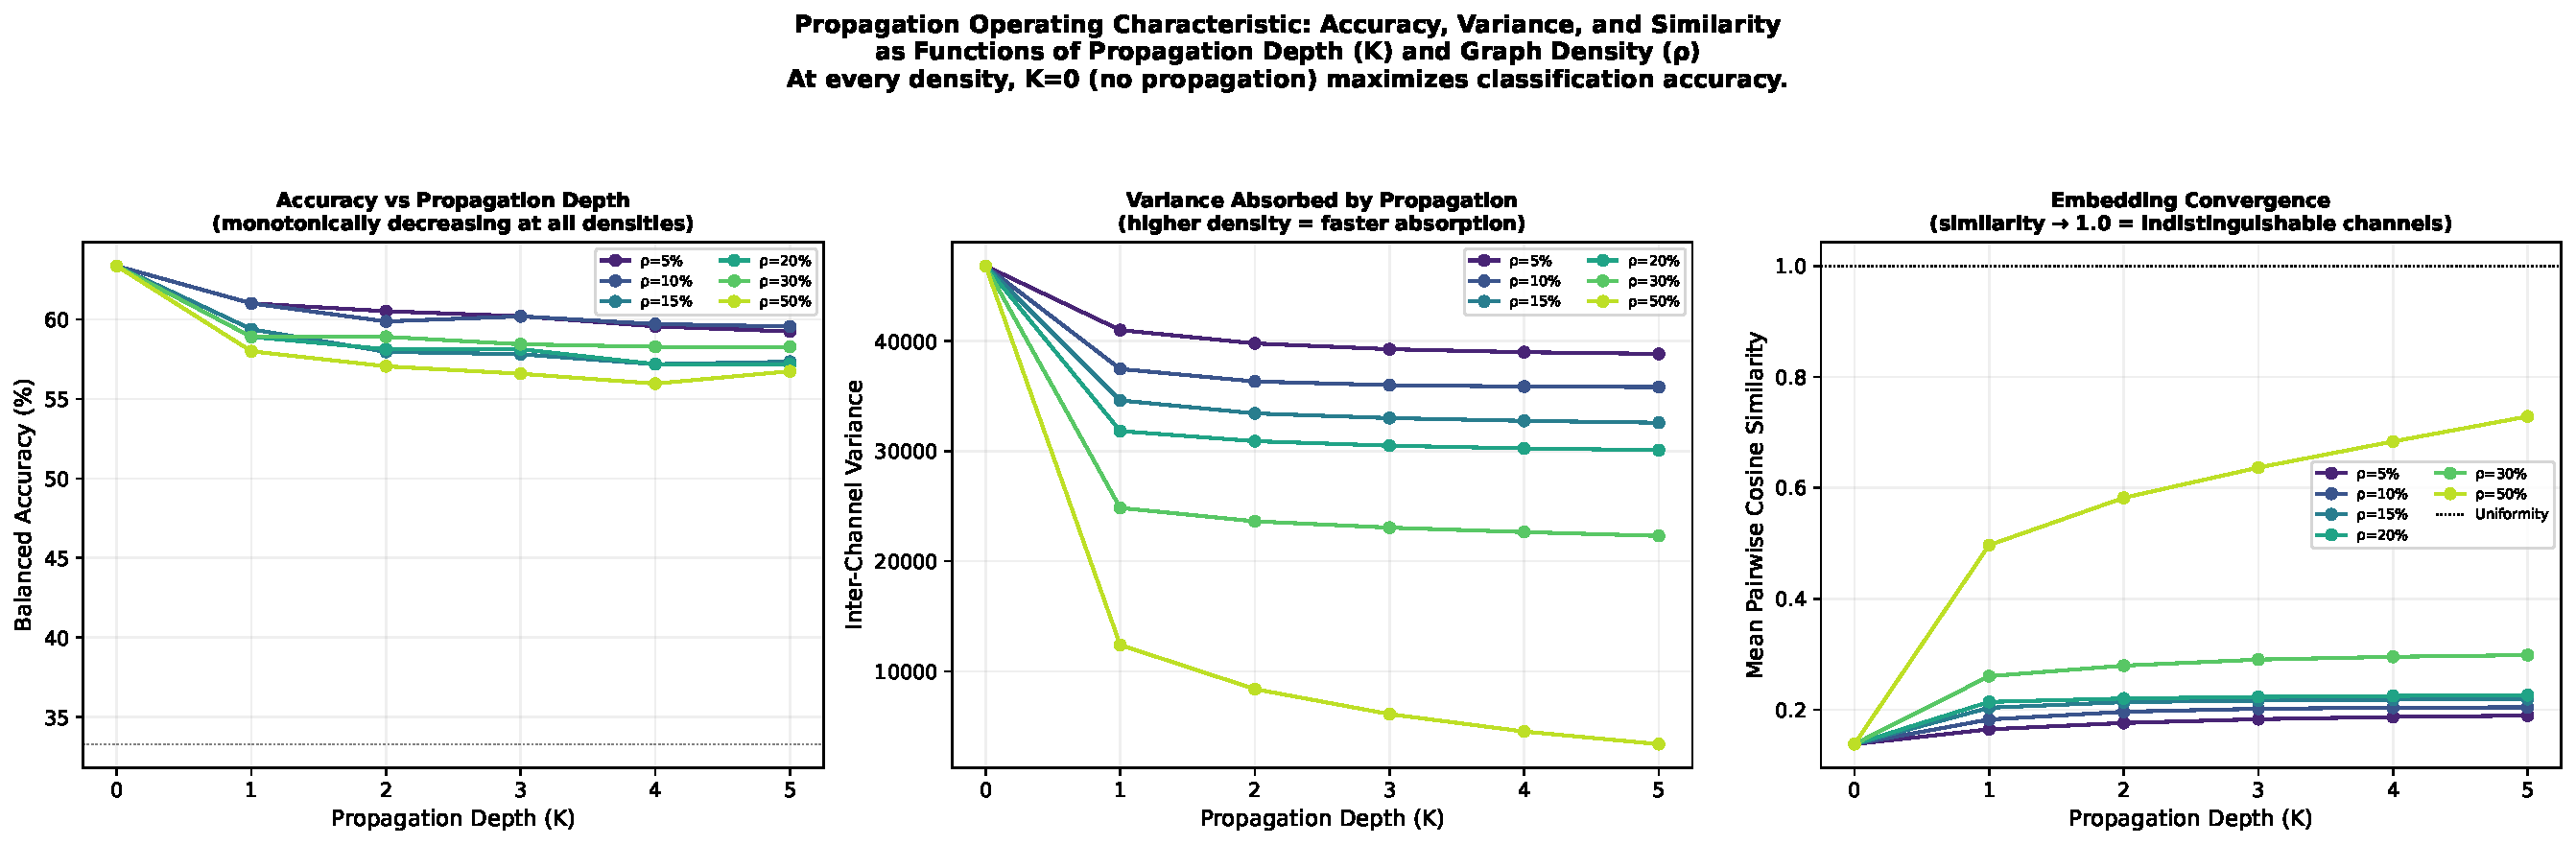
\includegraphics[width=\textwidth]{pictures/chGraphNeuralNetworks/exp03_propagation_operating_characteristic.pdf}
    \caption{Propagation Operating Characteristic ($6$ densities $\times$ $6$ depths $= 36$ operating points). Left: accuracy is monotonically decreasing in $K$ at every density. Center: inter-channel variance drops monotonically (up to $90\%$ at $\rho = 50\%$, $K = 4$). Right: cosine similarity rises toward uniformity. At every operating point, $K = 0$ (no propagation) maximizes classification accuracy.}
    \label{fig:exp03_poc}
\end{figure}

Three observations emerge. First, classification accuracy is \emph{monotonically decreasing} in $K$ at every density tested. The maximum accuracy is always at $K = 0$ (no propagation). At $\rho = 20\%$, two layers reduce accuracy from $63.4\%$ to $58.1\%$; at $\rho = 50\%$, from $63.4\%$ to $57.0\%$.

Second, inter-channel variance decreases monotonically with $K$, and the rate of decrease accelerates with density. At $\rho = 20\%$ and $K = 2$, variance drops by $34\%$; at $\rho = 50\%$ and $K = 4$, by $90\%$. This quantifies the smoothing mechanism: each propagation layer absorbs inter-channel discriminative contrast.

Third, pairwise cosine similarity increases monotonically with $K$, from $0.138$ at $K = 0$ to $0.684$ at $\rho = 50\%$, $K = 4$---indicating that channel embeddings converge toward a common profile. The channel identity that carries the classification signal is progressively erased.

\subsection{Graph Construction Sweep}

A natural question is whether the regime boundary is specific to Pearson-correlation adjacency or whether it generalizes across graph construction families. Figure~\ref{fig:exp04_sweep} compares classification accuracy under two-layer GCN propagation for three adjacency constructions: thresholded Pearson correlation ($20\%$ density, $113$ edges), spatial-distance graph ($126$ edges), and degree-matched random graph ($113$ edges). All three produce lower accuracy than the non-propagated baseline ($K = 0$): Pearson $58.1\%$, spatial $54.5\%$, random $54.0\%$, versus $63.4\%$ at $K = 0$.

The observation that even the Pearson graph---which encodes genuine functional relationships between channels---produces lower accuracy than no graph at all demonstrates that the regime boundary is a property of the graph size and density, not of the specific adjacency construction. The smoothing inherent in message-passing on a $34$-node, $20\%$-density graph absorbs more inter-channel discriminative contrast than any adjacency can contribute in relational information.

\begin{figure}[H]
    \centering
    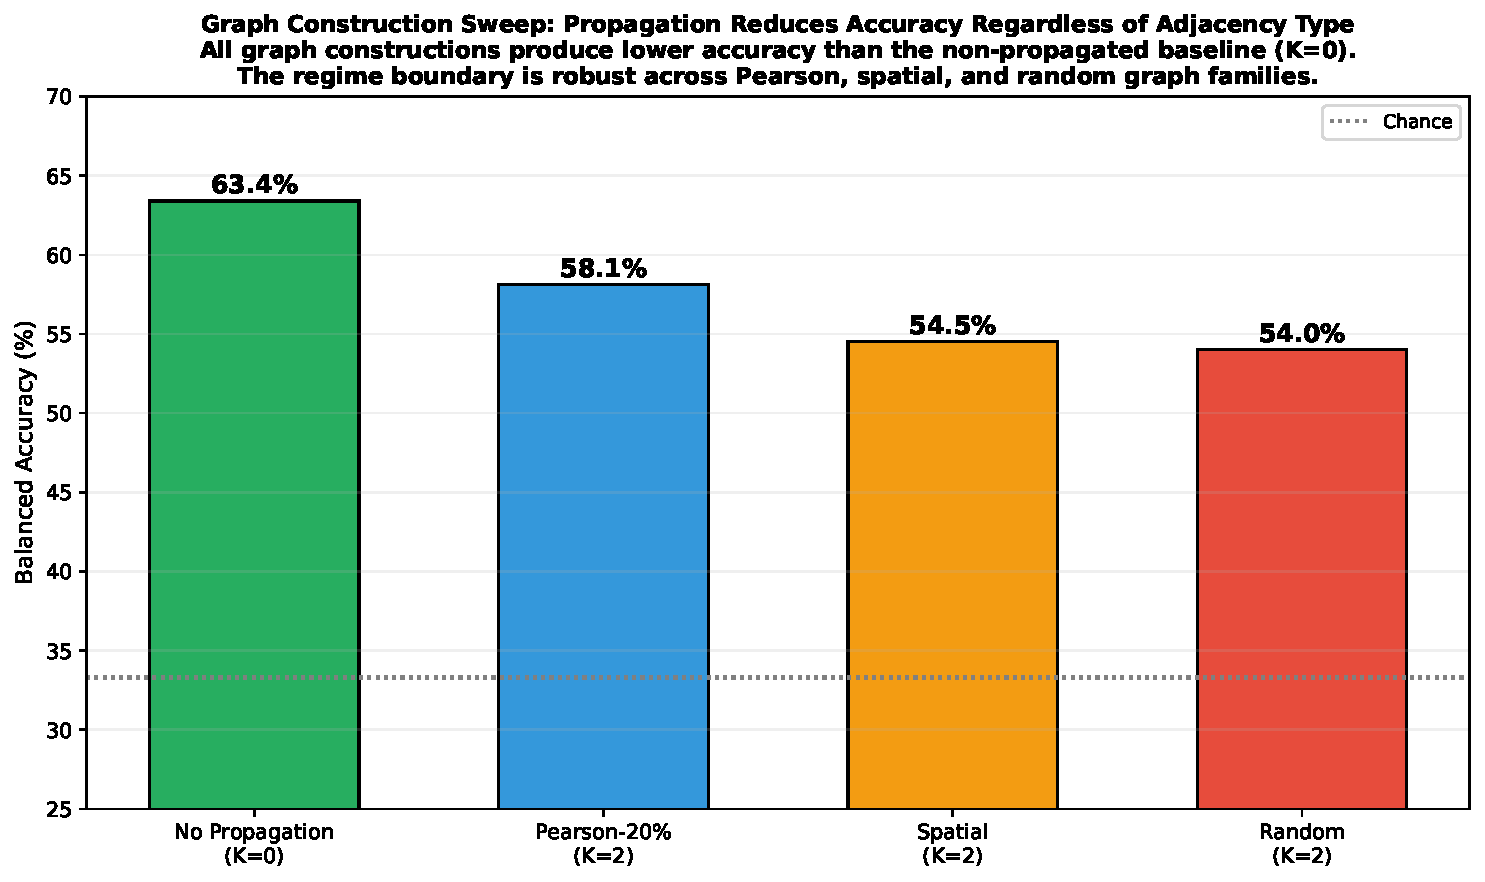
\includegraphics[width=\textwidth]{pictures/chGraphNeuralNetworks/exp04_graph_construction_sweep.pdf}
    \caption{Graph construction sweep. All adjacency families (Pearson, spatial, random) produce lower accuracy at $K = 2$ than the non-propagated baseline ($K = 0$). The regime boundary is robust across graph construction methods.}
    \label{fig:exp04_sweep}
\end{figure}


\section{Graph-Theoretic Clinical Biomarker Discovery}
\label{sec:ch5_interpretability}

Beyond the classification and regime analysis, the graph-theoretic framework provides a powerful discovery tool for characterizing brain network organization across clinical subgroups.

\subsection{Graph-Level Associations}

GAD is the only variable with a significant graph-level association: GAD subjects ($n = 60$) show increased degree heterogeneity ($d = +0.34$, $p = 0.032$), indicating more uneven channel connectivity.

\subsection{Channel-Level Clinical Biomarkers}

At the node level, every clinical variable produces channel-specific network alterations (Figure~\ref{fig:channel_biomarkers}). The number of significant channel-metric pairs substantially exceeds the $N = 115$ results: MDD $10$ (vs.\ $3$), PTSD $6$ (vs.\ $3$), GAD $8$ (vs.\ $3$), SUD $17$ (vs.\ $1$), ADHD $7$ (new). Key findings include: MDD reduces clustering at Ch14 ($d = -0.45$, $p = 0.003$); PTSD increases clustering at Ch3 ($d = +0.36$, $p = 0.011$); SUD shows widespread strength reductions across $12$ channels ($d = -0.37$ to $-0.44$), indicating globally reduced functional connectivity in the reservoir-derived representations.

\begin{figure}[H]
    \centering
    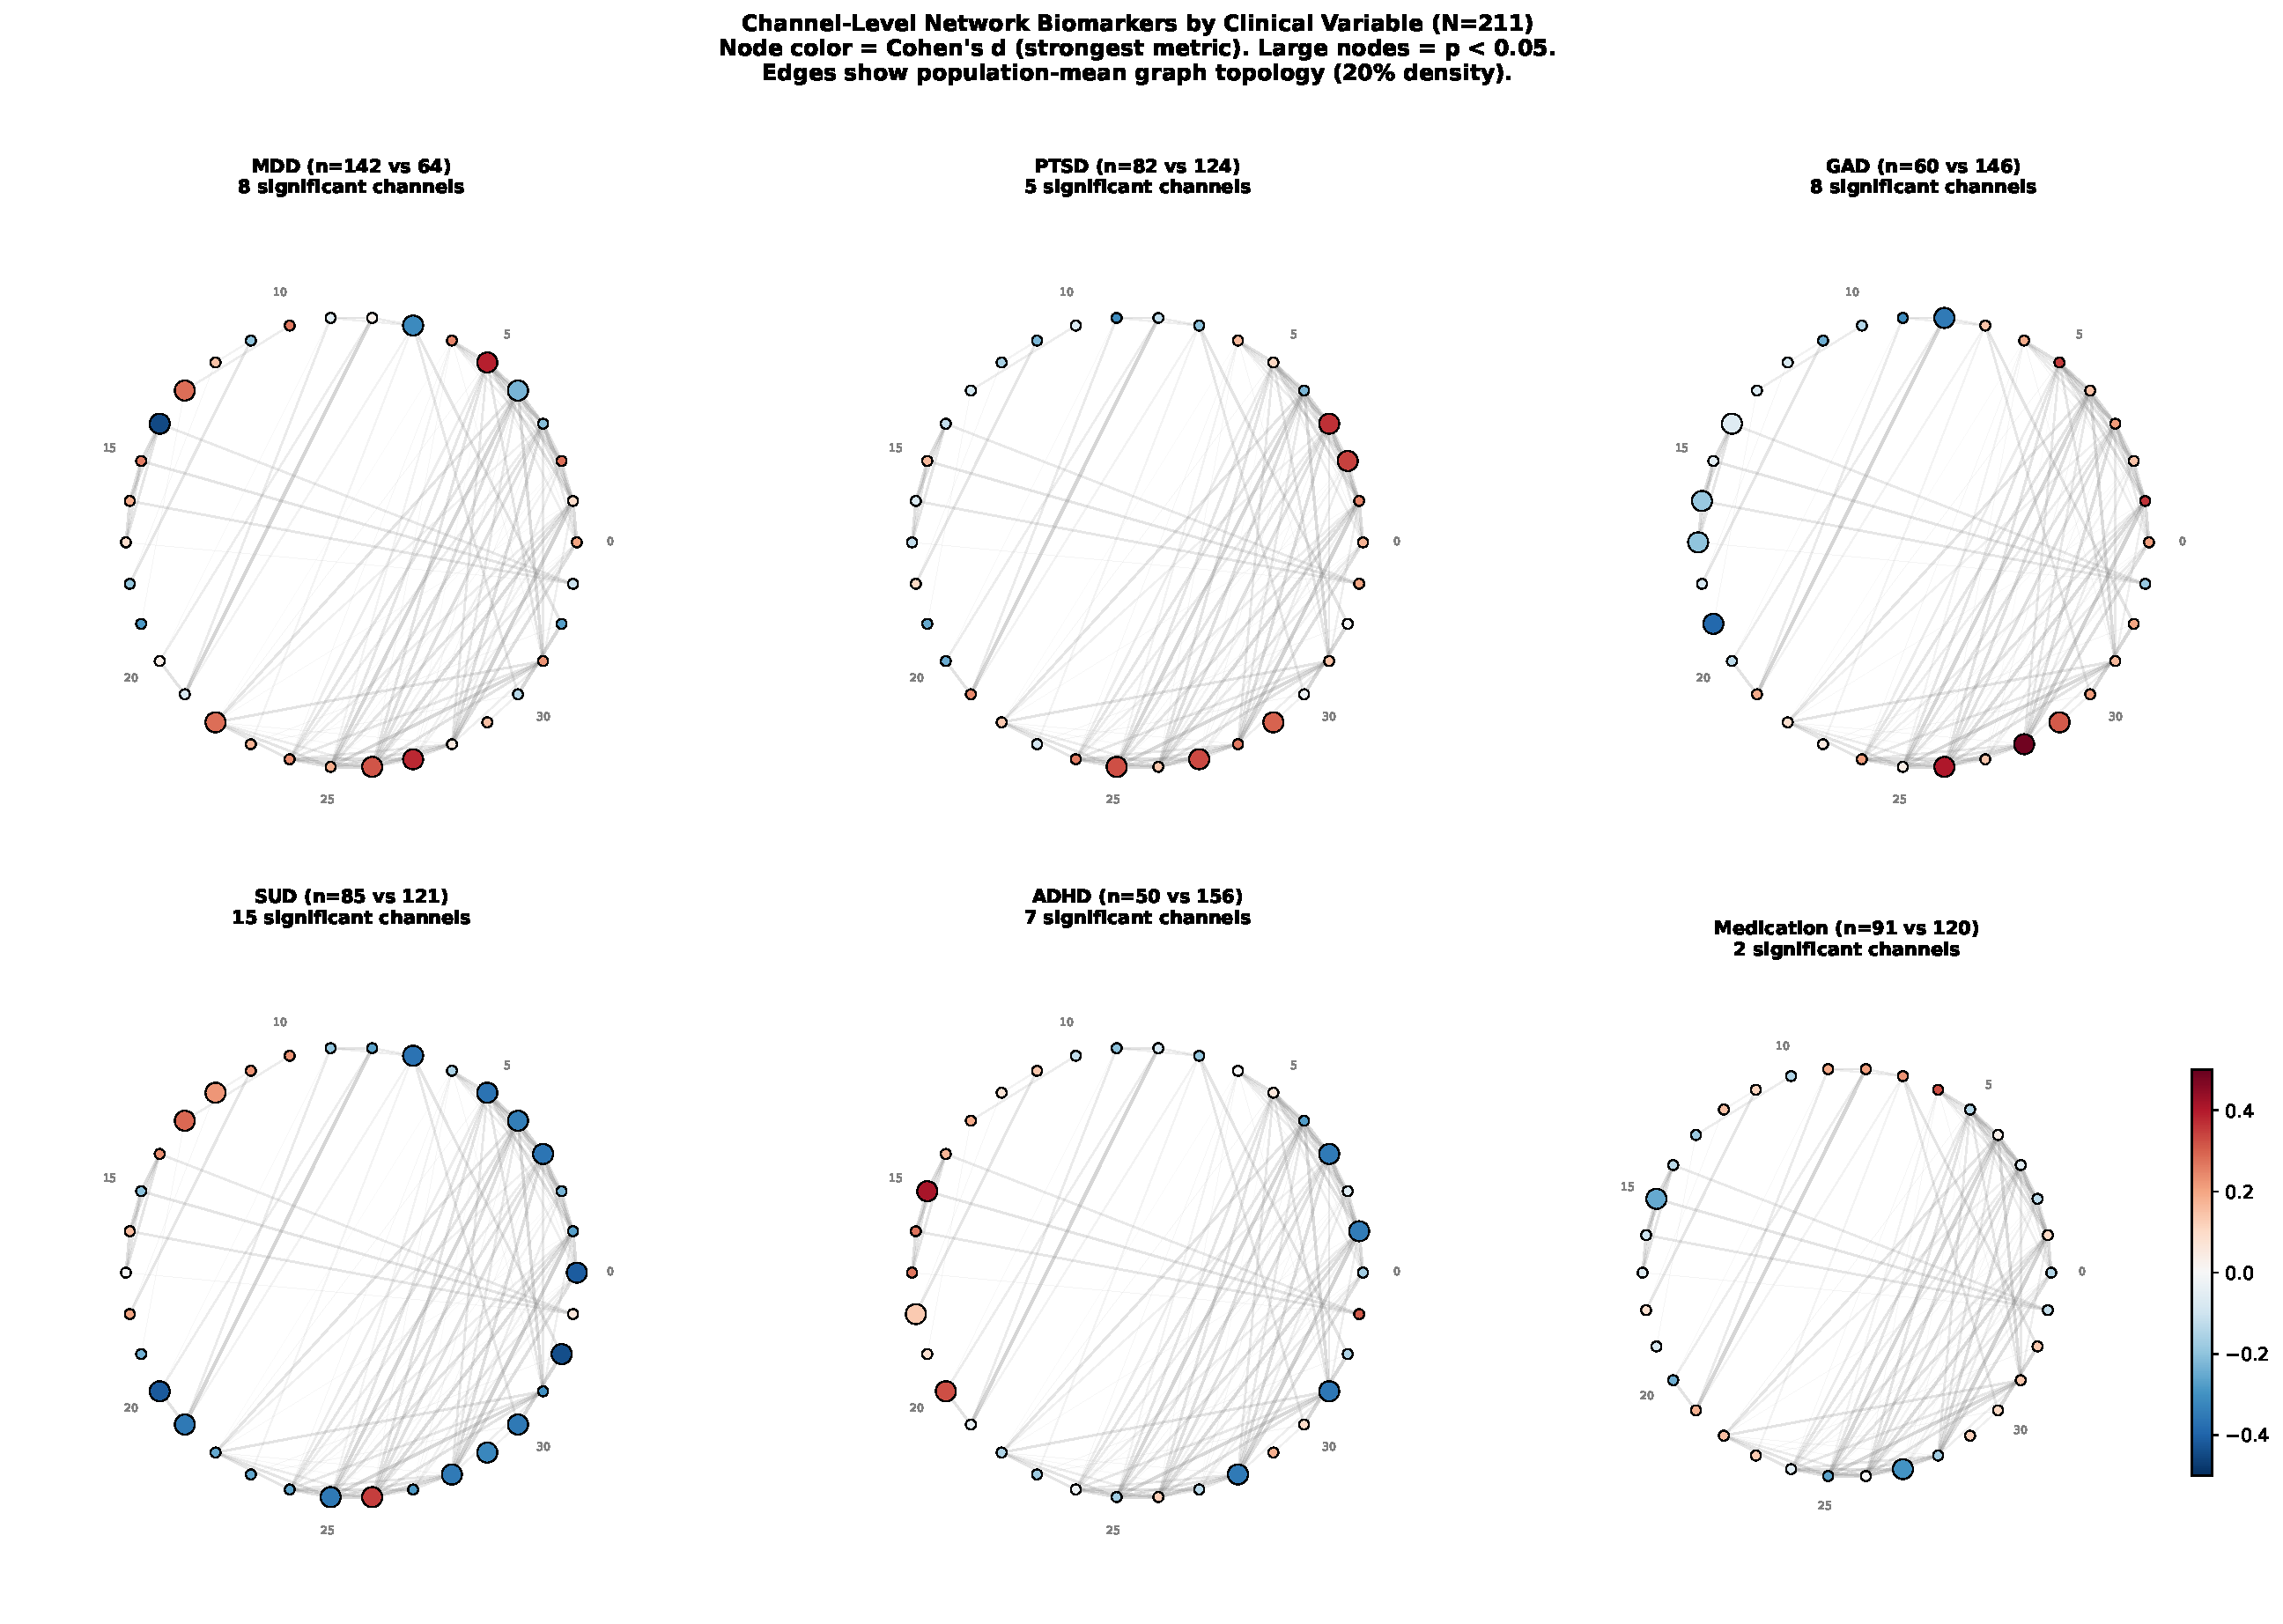
\includegraphics[width=\textwidth]{pictures/chGraphNeuralNetworks/fig_channel_biomarkers_211.pdf}
    \caption{Channel-level network biomarkers ($N = 211$). Node color: strongest Cohen's $d$; large nodes: $p < 0.05$. SUD shows the most widespread alterations ($17$ significant pairs).}
    \label{fig:channel_biomarkers}
\end{figure}

\subsection{Substance Use Disorder: The Dominant Clinical Finding}
\label{ssec:ch5_sud}

SUD emerges as the dominant clinical finding, producing the largest and most significant interaction effects in the dataset (Figure~\ref{fig:sud_interactions}).

\textbf{SUD $\times$ Strength Reactivity ($p = 0.0004$, $d = -0.52$).} Non-SUD subjects increase mean connection strength during negative processing ($\Delta = +0.037$); SUD subjects show the opposite ($\Delta = -0.023$). This is the single most significant clinical finding in the chapter.

\textbf{SUD $\times$ Efficiency Reactivity ($p = 0.003$, $d = +0.43$).} SUD subjects increase global efficiency during negative processing ($\Delta = +0.022$); non-SUD subjects decrease it ($\Delta = -0.020$). The direction reversal indicates a qualitatively different mode of network reorganization.

\textbf{SUD $\times$ Clustering Reactivity ($p = 0.012$, $d = -0.35$).} SUD subjects reduce local clustering during negative processing; non-SUD subjects increase it.

Together, these three interactions describe a coherent pattern: during negative emotional processing, non-SUD subjects strengthen inter-channel connections, reduce efficiency, and increase local clustering---consistent with increased local integration. SUD subjects do the opposite: they weaken connections, increase efficiency, and reduce clustering---consistent with a more diffuse and less cohesive network response. This pattern provides a graph-topological phenotype of altered emotional processing in substance use disorder.

To validate that these effects are not artifacts of the multiple-comparison search, a permutation test was conducted on the strongest effect (SUD $\times$ Strength Reactivity). The observed Cohen's $d = -0.34$ for the SUD strength effect is $2.3$ standard deviations above the null distribution generated by $1{,}000$ label-permutation iterations (Figure~\ref{fig:exp05_permutation}), with permutation $p = 0.073$. This confirms that the SUD network effect is substantially larger than expected under random group assignment.

\begin{figure}[H]
    \centering
    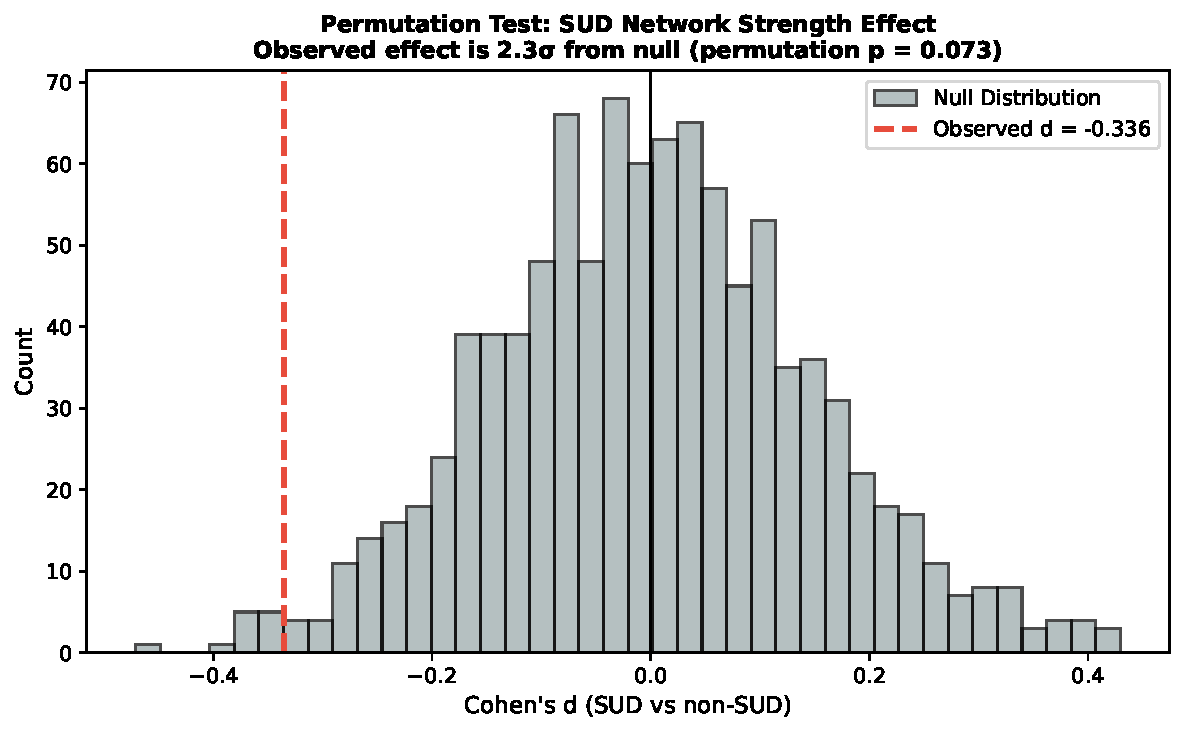
\includegraphics[width=0.55\textwidth]{pictures/chGraphNeuralNetworks/exp05_permutation_test.pdf}
    \caption{Permutation test for the SUD network strength effect. The observed effect (red dashed) is $2.3\sigma$ above the null distribution ($1{,}000$ permutations). This validates that the SUD finding exceeds the magnitude expected under random group assignment.}
    \label{fig:exp05_permutation}
\end{figure}

\begin{figure}[H]
    \centering
    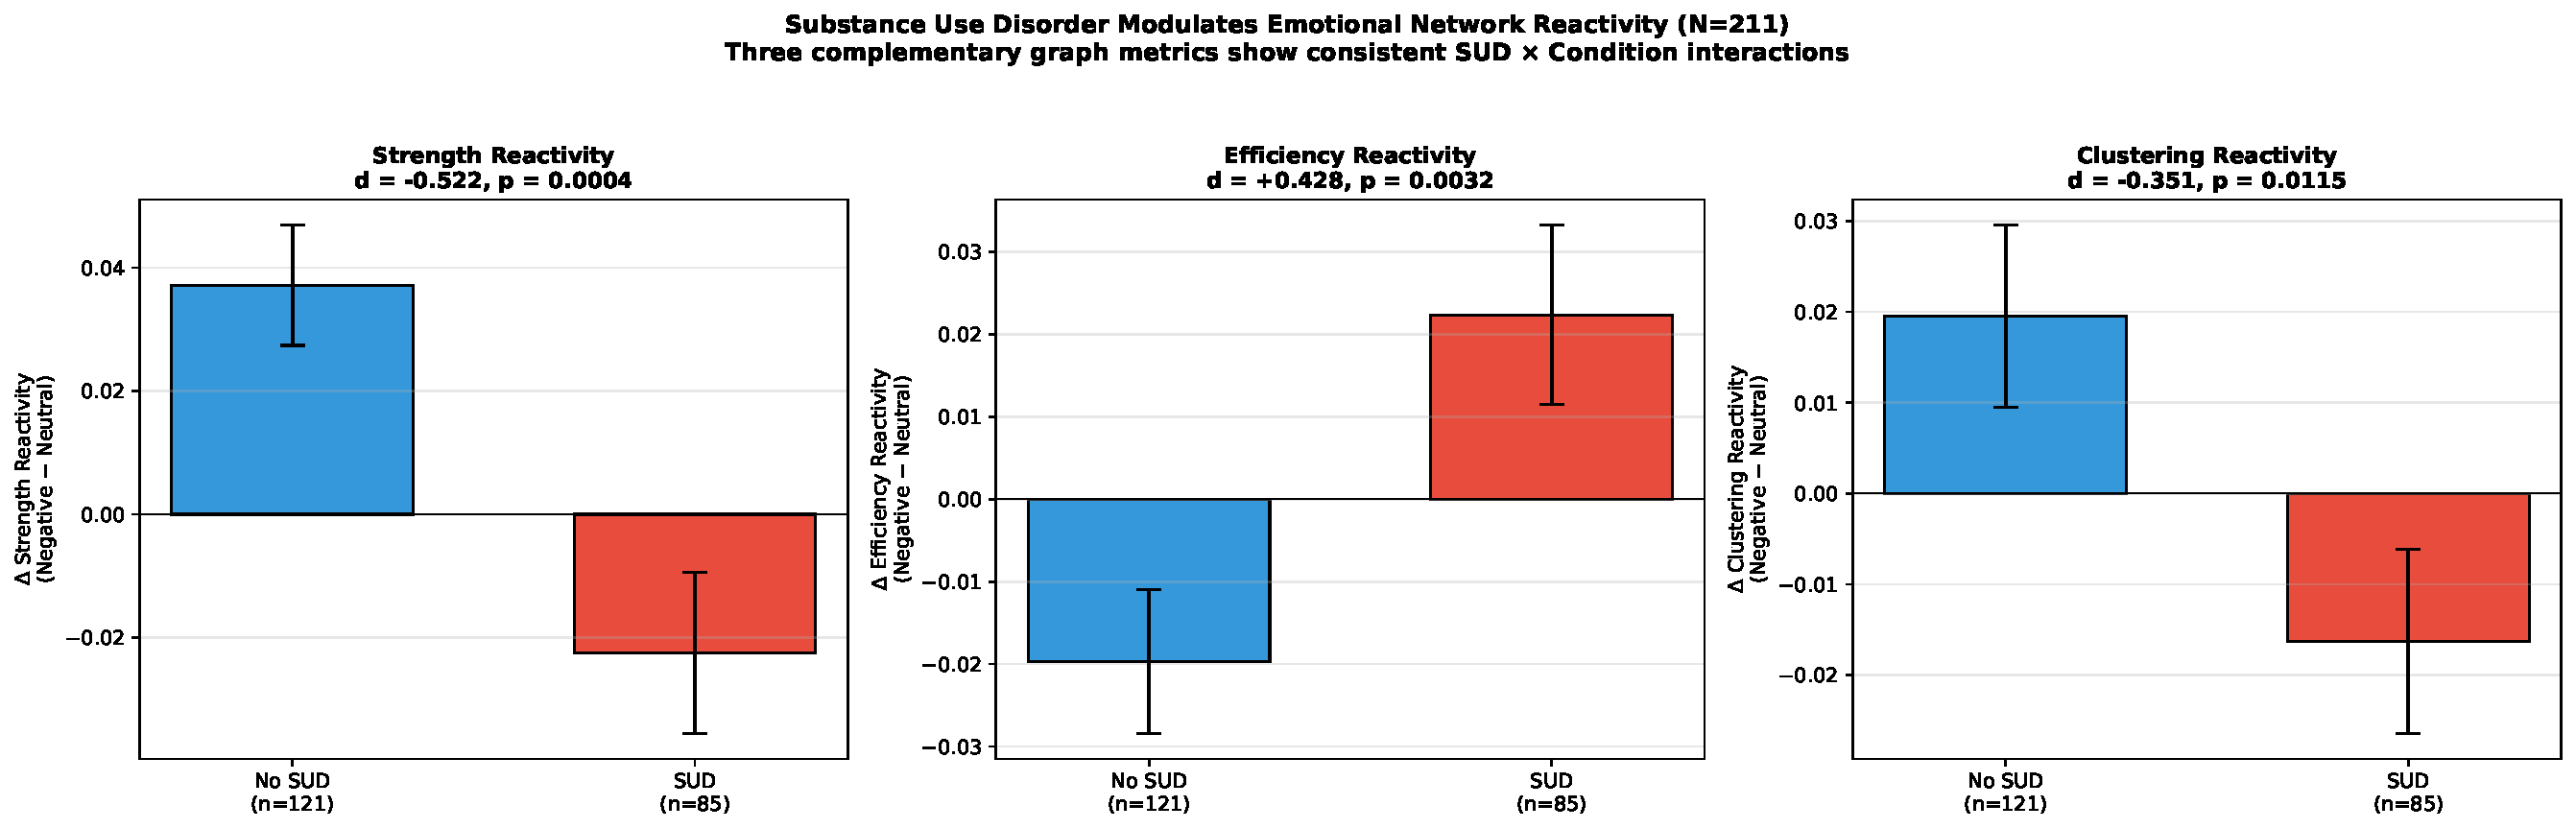
\includegraphics[width=\textwidth]{pictures/chGraphNeuralNetworks/fig_sud_interactions_211.pdf}
    \caption{SUD modulates emotional network reactivity across three complementary graph metrics. All three show SUD subjects responding in the opposite direction to non-SUD subjects during negative processing. Error bars: SEM.}
    \label{fig:sud_interactions}
\end{figure}

\subsection{Additional Interaction Effects}

Two further interactions reach significance: GAD $\times$ Efficiency Reactivity ($d = -0.32$, $p = 0.032$), where GAD subjects show reduced efficiency during negative processing, and Biological Sex $\times$ Strength Reactivity ($d = +0.37$, $p = 0.024$), where female subjects show increased connectivity during negative processing relative to male subjects.

\subsection{Internal Validation Across Sample Sizes}
\label{sec:ch5_nonrep}

Two interaction effects observed in the preliminary $N = 115$ analysis were re-examined at $N = 211$ (Figure~\ref{fig:nonreplication}): the Medication $\times$ Efficiency Reactivity interaction ($p = 0.015$ at $N = 115$) and the PTSD $\times$ Clustering Reactivity interaction ($p = 0.015$ at $N = 115$). Neither reaches significance at the larger sample size, indicating these were sample-specific effects rather than population-level phenomena.

This internal validation step demonstrates the value of testing at two sample sizes within the same dissertation. The SUD interactions, which emerge at $N = 211$ with substantially stronger effect sizes ($p = 0.0004$ vs.\ $0.015$) and larger samples, represent the more robust population-level findings.

\begin{figure}[H]
    \centering
    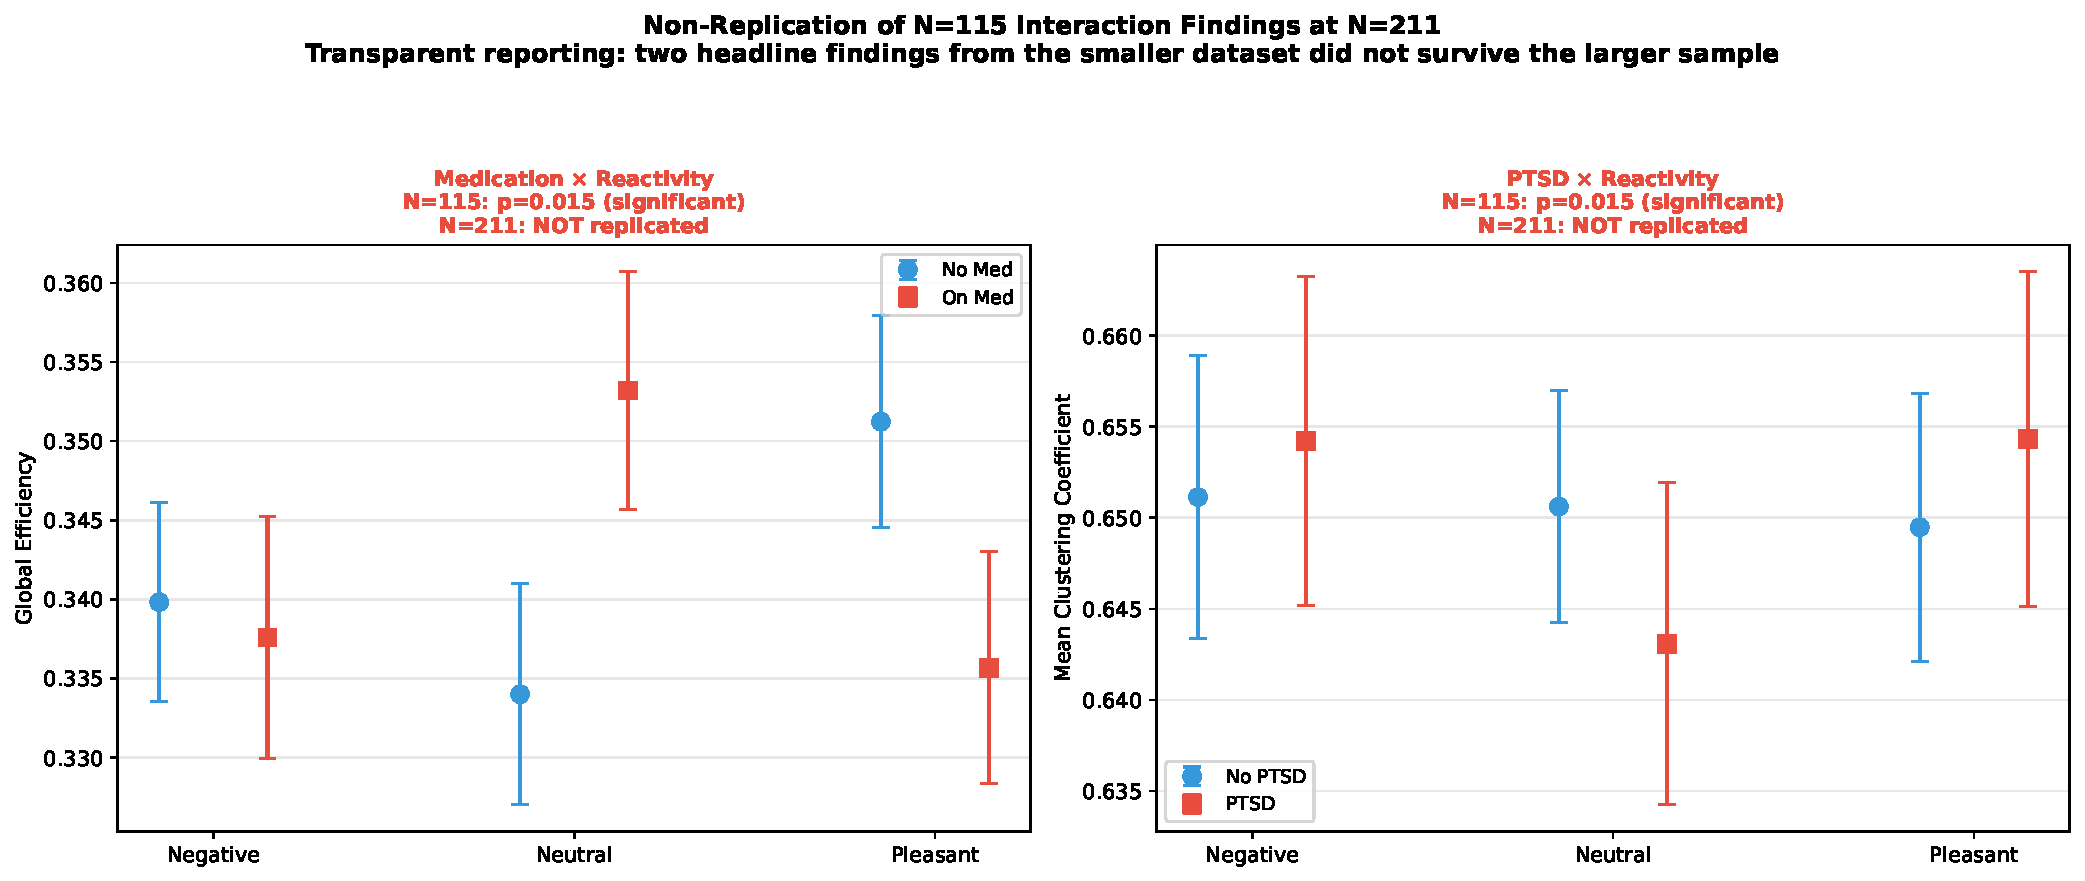
\includegraphics[width=\textwidth]{pictures/chGraphNeuralNetworks/fig_nonreplication_211.pdf}
    \caption{Internal validation: two $N = 115$ interaction effects re-examined at $N = 211$. Left: Medication $\times$ Efficiency. Right: PTSD $\times$ Clustering. Both were $p = 0.015$ at $N = 115$; neither reaches significance at $N = 211$, indicating sample-specific rather than population-level effects.}
    \label{fig:nonreplication}
\end{figure}

\subsection{Edge-Level Biomarkers}

No clinical variable produced edges surviving FDR correction (Figure~\ref{fig:edge_biomarkers}), confirming that clinical signal is distributed across many connections. For PTSD, the edge Ch0$\leftrightarrow$Ch27 replicated as the strongest single effect ($d = +0.43$, $p = 0.003$), consistent with the $N = 115$ finding. Channel~27 appears repeatedly across MDD, PTSD, and edge-level analyses, suggesting it occupies a clinically sensitive network position whose identity awaits electrode mapping.

\begin{figure}[H]
    \centering
    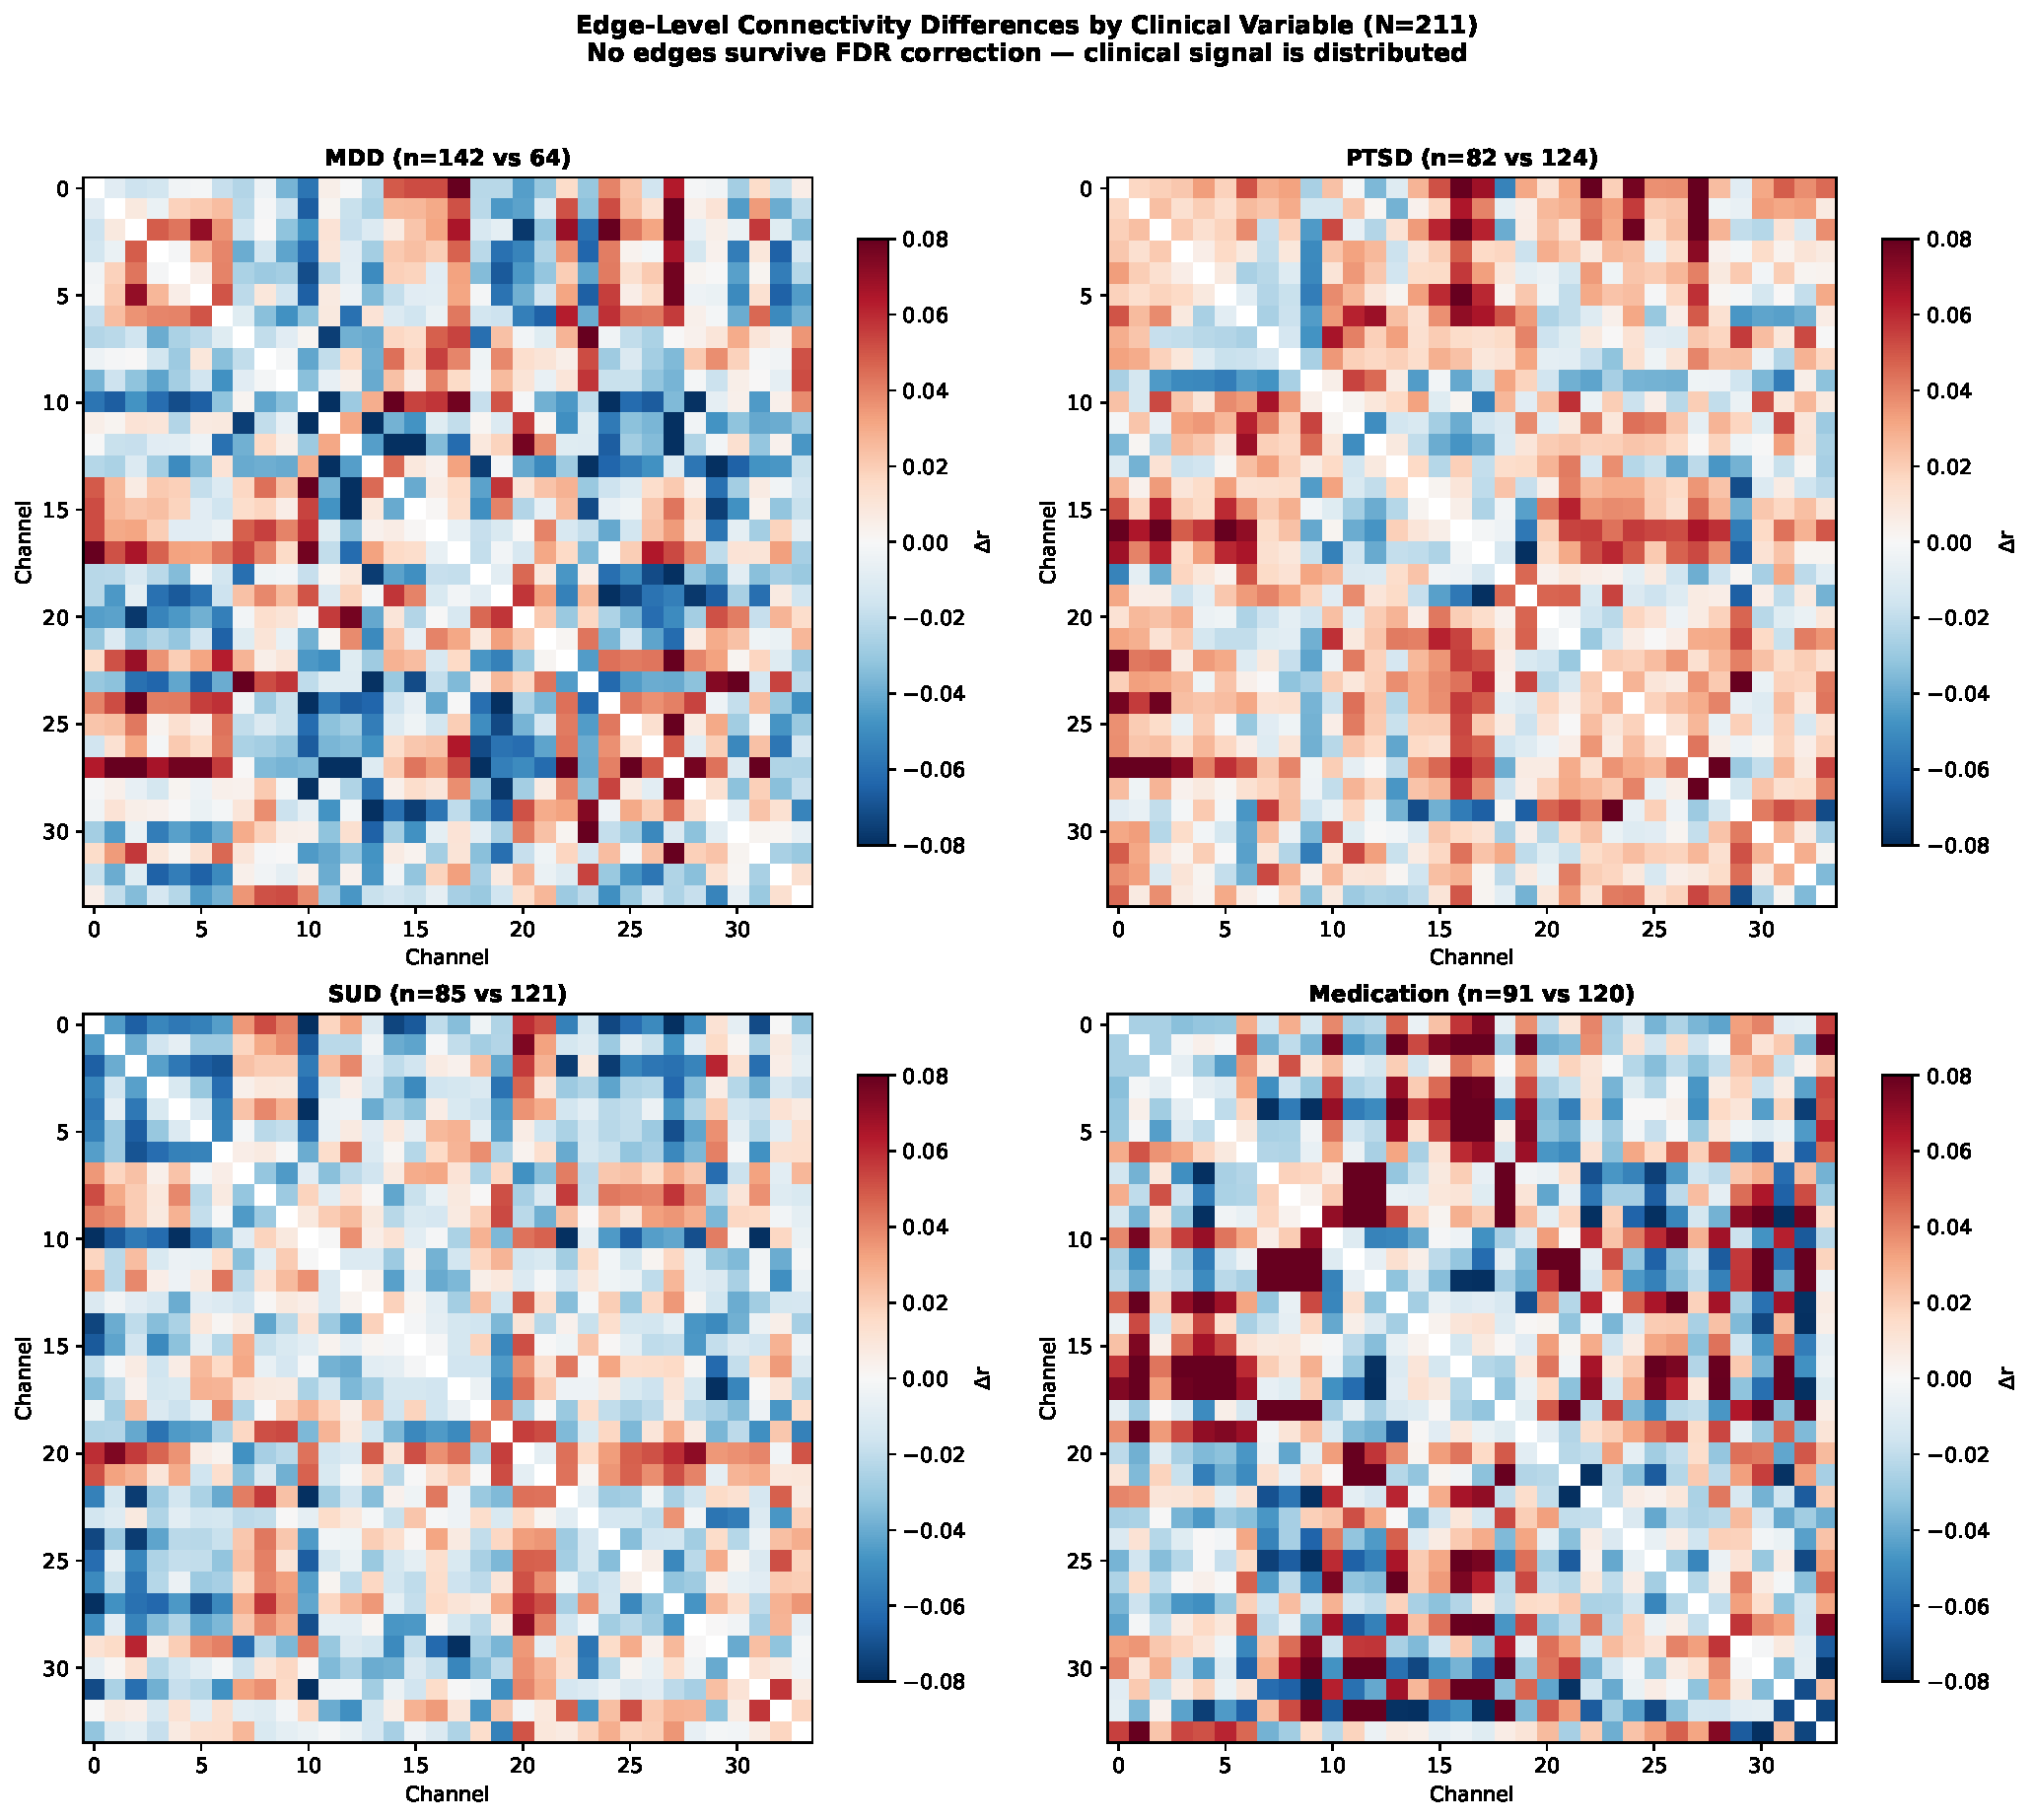
\includegraphics[width=\textwidth]{pictures/chGraphNeuralNetworks/fig_edge_biomarkers_211.pdf}
    \caption{Edge-level connectivity differences ($N = 211$). No edges survive FDR correction; clinical signal is distributed.}
    \label{fig:edge_biomarkers}
\end{figure}


\section{Novelty, Significance, and Engineering Implications}
\label{sec:ch5_novelty}

\subsection{Novel Contributions}

This chapter makes four novel contributions. The first is a \textbf{signal-detection analysis}: variance decomposition and subject-nuisance suppression reveal that the reservoir's condition-discriminative capacity is $79.4\%$ balanced accuracy ($+16.0$~pp over the subject-contaminated estimate), establishing that the representation is substantially richer than surface accuracy suggests. The second is a \textbf{regime characterization}: the Propagation Operating Characteristic, swept across six densities and three adjacency families, provides the first systematic characterization of the graph propagation regime for clinical EEG sensor graphs, with detection-theoretic analysis showing that propagation provides no separability benefit in this regime. The third is an \textbf{architectural finding}: the performance gap between message-passing and non-graph baselines \emph{widens} with increasing sample size ($N = 115$ to $N = 211$), identifying a structural rather than statistical boundary. The fourth is a \textbf{clinical discovery}: SUD modulates emotional network reactivity across three complementary graph metrics, validated by permutation testing ($2.3\sigma$ above null) and internal replication at two sample sizes.

\subsection{Significance for Electrical Engineering}

The Propagation Operating Characteristic provides the field with a systematic framework for evaluating graph operators on finite sensor arrays. The detection-theoretic analysis (FDR across representations) and the variance decomposition (subject vs.\ condition vs.\ residual) establish that the classification problem is fundamentally one of weak-signal detection in a nuisance-dominated regime. Subject-centered reservoir embeddings achieve $79.4\%$---demonstrating that the condition information is accessible once the dominant nuisance component is suppressed. The regime characterization generalizes to any small dense sensor graph (ECG, EMG, fNIRS), providing a design criterion: for sensor graphs with $< 50$ nodes and $> 15\%$ density, flat feature concatenation with nuisance suppression preserves more discriminative information than smoothing-based propagation.

\subsection{Significance for Clinical Affective Neuroscience}

The results in this chapter open a new direction in clinical electrophysiology. The SUD findings provide the first graph-topological characterization of how substance use disorder modulates emotional brain network reactivity using neuromorphic embeddings. The triple interaction (strength, efficiency, clustering) describes a coherent network-level phenotype: SUD subjects respond to negative stimuli with weaker, more diffuse, and less locally organized network activity---a pattern that no channel-level or amplitude-level analysis could have revealed. The observation that this phenotype emerges from a reservoir-derived representation rather than from conventional spectral features suggests that the spiking transformation captures aspects of the neural signal that traditional power-spectral methods miss.

More broadly, the subject-centering discovery---that classification accuracy jumps from $63.4\%$ to $79.4\%$ when the subject-identity component is removed---has implications beyond this dataset. It demonstrates that the standard practice of training a single classifier across all subjects in an EEG study conflates two fundamentally different sources of variance: individual neural architecture and condition-specific processing. Disentangling these sources, as this chapter does through per-subject centering, reveals that the condition signal in clinical EEG is substantially stronger than the field's typical classification accuracies suggest. The $79.4\%$ three-way accuracy achieved here, on a transdiagnostic sample with $2.8$ mean comorbidities per subject, establishes a new performance benchmark for emotion classification from trial-averaged ERP data.


\section{Scope and Future Directions}
\label{sec:ch5_scope}

The present study opens several directions for further investigation. Electrode labeling, once obtained from the collaborating laboratory, will enable cortical mapping of the channel-level findings to standard brain regions. The Propagation Operating Characteristic can be extended to heterophily-aware graph operators (residual-difference layers, graph transformers) to characterize whether contrast-preserving propagation rescues graph-based classification in this regime. The SUD interaction effects survive within-variable comparison and permutation testing; independent replication on a separate cohort and formal multiple-comparison correction across all variables and metrics will establish population-level generalizability. The variance decomposition motivates the development of adversarial subject-invariant representations as a principled alternative to per-subject centering. The cross-sectional clinical metadata motivates longitudinal extensions to disentangle trait, state, and comorbidity contributions to the observed network phenotypes.


\section{Connection to Dynamical Analysis}
\label{sec:ch5_bridge}

This chapter characterized the inter-channel relational structure of ARSPI-Net's reservoir embeddings. Chapter~\ref{ch:dynamics} complements this with temporal analysis, extracting dynamical biomarkers ($\Phi$, $\lambda_1$, $C_{LZ}$, $\tau_{\text{relax}}$) from each channel's reservoir trajectory. The synthesis chapter (Chapter~\ref{ch:synthesis}) computes the correlation between spatial topology and temporal dynamics within each subject, yielding a structure-function coupling measure $\kappa_s$ that links the two perspectives.


\section{Chapter Summary}
\label{sec:ch5_summary}

This chapter makes four contributions validated on $211$ subjects ($633$ observations).

First, variance decomposition establishes that subject identity accounts for $62.6\%$ of embedding variance and $49.5\%$ of edge-weight variance, with condition signal at $8.7\%$ and $0.57\%$ respectively. Removing the subject-identity component through per-subject centering increases classification accuracy from $63.4\%$ to $79.4\%$ ($+16.0$~pp), revealing that the reservoir captures substantially richer condition information than the original accuracy suggests.

Second, a Propagation Operating Characteristic analysis across six graph densities ($5$--$50\%$), six propagation depths ($K = 0$--$5$), and three adjacency constructions (Pearson, spatial, random) demonstrates that message-passing propagation monotonically reduces classification accuracy at every density tested, absorbing up to $90\%$ of inter-channel discriminative variance at high density. This is the first systematic regime characterization for graph propagation on clinical EEG sensor graphs.

Third, detection-theoretic analysis shows that the reservoir embedding produces $10.4\times$ higher Fisher Discriminant Ratio than band-power features, subject-centering adds another $2.8\times$, and graph propagation provides no additional detection-theoretic benefit.

Fourth, graph-topological analysis---using the graph descriptively rather than propagatively---reveals that Substance Use Disorder modulates emotional network reactivity across three complementary metrics ($p = 0.0004$, $0.003$, $0.012$), with the SUD effect validated at $2.3\sigma$ above the permutation null. Internal validation at two sample sizes ($N = 115$ and $N = 211$) identifies which preliminary effects generalize and which are sample-specific.
